\documentclass[swedish]{beamer}
\usepackage{pgfpages}
\usepackage{myslides}
\usepackage{fancyvrb}
\usepackage[lighttt]{lmodern}
\usepackage{menukeys}
\usepackage{calc}

\usepackage{graphicx}

\lstset{language=bash}

\makeatletter
\AtBeginDocument{% 
   \@ifpackageloaded{fancyvrb}{}{\let\@xpace@fancyvrb@catcodes\relax}% 

} 

\def\@xpace@fancyvrb@catcodes{% 
   \ifx\relax \FV@CommandChars 
   \else 
     \expandafter\@xpace@fancyvrb@catcodes@aux\FV@CommandChars 
   \fi 
} 

\def\@xpace@fancyvrb@catcodes@aux 
   \catcode`#1=0\relax\catcode`#2=1\relax\catcode`#3=2\relax{% 
     \@makeother#1\@makeother#2\@makeother#3% 
} 

\def\@xspace@eTeX@setup{% 
   \begingroup 
   \everyeof{}% 
   \endlinechar=-1\relax 
   \@xpace@fancyvrb@catcodes % extra line here. 
   \catcode`\ =10\relax 
   \makeatletter 
   \catcode`\\\z@ 
   \catcode`\{\@ne 
   \catcode`\}\tw@ 
   \expandafter\scantokens\expandafter{\expandafter\gdef 
     \expandafter\@xspace@exceptions@tlp 
     \expandafter{\@xspace@exceptions@tlp}}% 
   \endgroup 
} 

\setkeys{Gin}{width= 
  \ifdim\Gin@nat@width>0.95\linewidth 0.95\linewidth \else 
\Gin@nat@width\fi} 
\setkeys{Gin}{height= 
  \ifdim\Gin@nat@height>0.95\textheight 0.95\textheight \else 
\Gin@nat@height\fi} 
\setkeys{Gin}{keepaspectratio=true} 


\makeatother

%\newenvironment{dialogue}{%
%\VerbatimEnvironment
%\begin{Verbatim}[fontsize=\footnotesize,commandchars=\#\(\)]%
%}
%{%
%\end{Verbatim}
%}

\title{Versionshantering och git}
\author{Kai-Mikael Jää-Aro}
\date{}


\begin{document}
\setlength{\intextsep}{0mm}
%\setbeameroption{show notes on second screen=left}

\begin{frame}
\titlepage
\end{frame}

\section{Introduktion}
\begin{frame}
  \frametitle{Problemet}
Mjukvaruutveckling är inte en linjär process från en tom fil till \(n\) rader korrekt fungerande kod.
\begin{itemize}
\item Fel införs under arbetets gång.
\item Vi provar alternativa lösningar.
\item Flera parallella versioner krävs.
\end{itemize}

Därför måste vi:
\begin{itemize}
\item kunna återgå till en fungerande version av mjukvaran,
\item arbeta med en av flera möjliga versioner.
\end{itemize}

\end{frame}

\begin{frame}
\frametitle{Versionskontroll är lösningen} 
  \begin{itemize}
  \item Ett arkiv.
  \item\emph{Incheckning} av kod (\emph{revisioner}) i arkivet.
  \item Hämta ut tidigare incheckningar.
  \item  Trädstruktur för parallella
    versioner. (``tip''/``trunk''/``master'' är huvudspåret.)
  \item Ändringar i parallella versioner kan föras tillbaka till master.
  \item Varje revision har en identitet, kan markeras med en \emph{tag} som 
motsvarar släppt version eller annan milsten. 
  \end{itemize}
\end{frame}

\begin{frame}
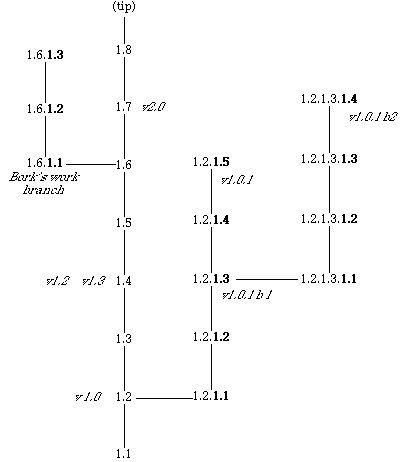
\includegraphics{revision-tree}
\end{frame}

\begin{frame}
\frametitle{Parallell utveckling}

Flera utvecklare i samma projekt.
\begin{enumerate}
\item Checka ut aktuell version av koden.
\item Koda, testa.
\item Checka in \emph{stabil} kod.
\item Hantera ev konflikter.
\item Repetera tills projektet klart.
\end{enumerate}
\end{frame}

\section{Git}
\begin{frame}
\frametitle{Git}
Det finns ett stort antal versionshanteringssystem, här kommer vi att gå igenom git.

  git är ett \emph{distribuerat} versionskontrollsystem.  \Mao lagrar \emph{alla} utvecklare en (komprimerad) kopia av hela databasen, men normalt utser man ett specifikt arkiv till att vara ``origin'', till vilket alla kopierar sitt material och som alla hämtar ifrån.

Dock är man inte beroende av det centrala arkivet utan kan arbeta offline med sin kopia tills man får kontakt med arkivet igen.

\end{frame}

\begin{frame}
  \frametitle{Att använda git}
Grunden för git är ett kommandoradsgränssnitt. Det finns flera olika
grafiska gränssnitt. (Mera avancerade övningar kräver användning av kommandotolken)

GitHub (\url{https://github.com/}) gör tillgängligt både ett grafiskt gränssnitt till git och gratis server-utrymme för open source-projekt.

\end{frame}

\section{Att sätta upp Git}
\begin{frame}
\frametitle{Skapa en användare}
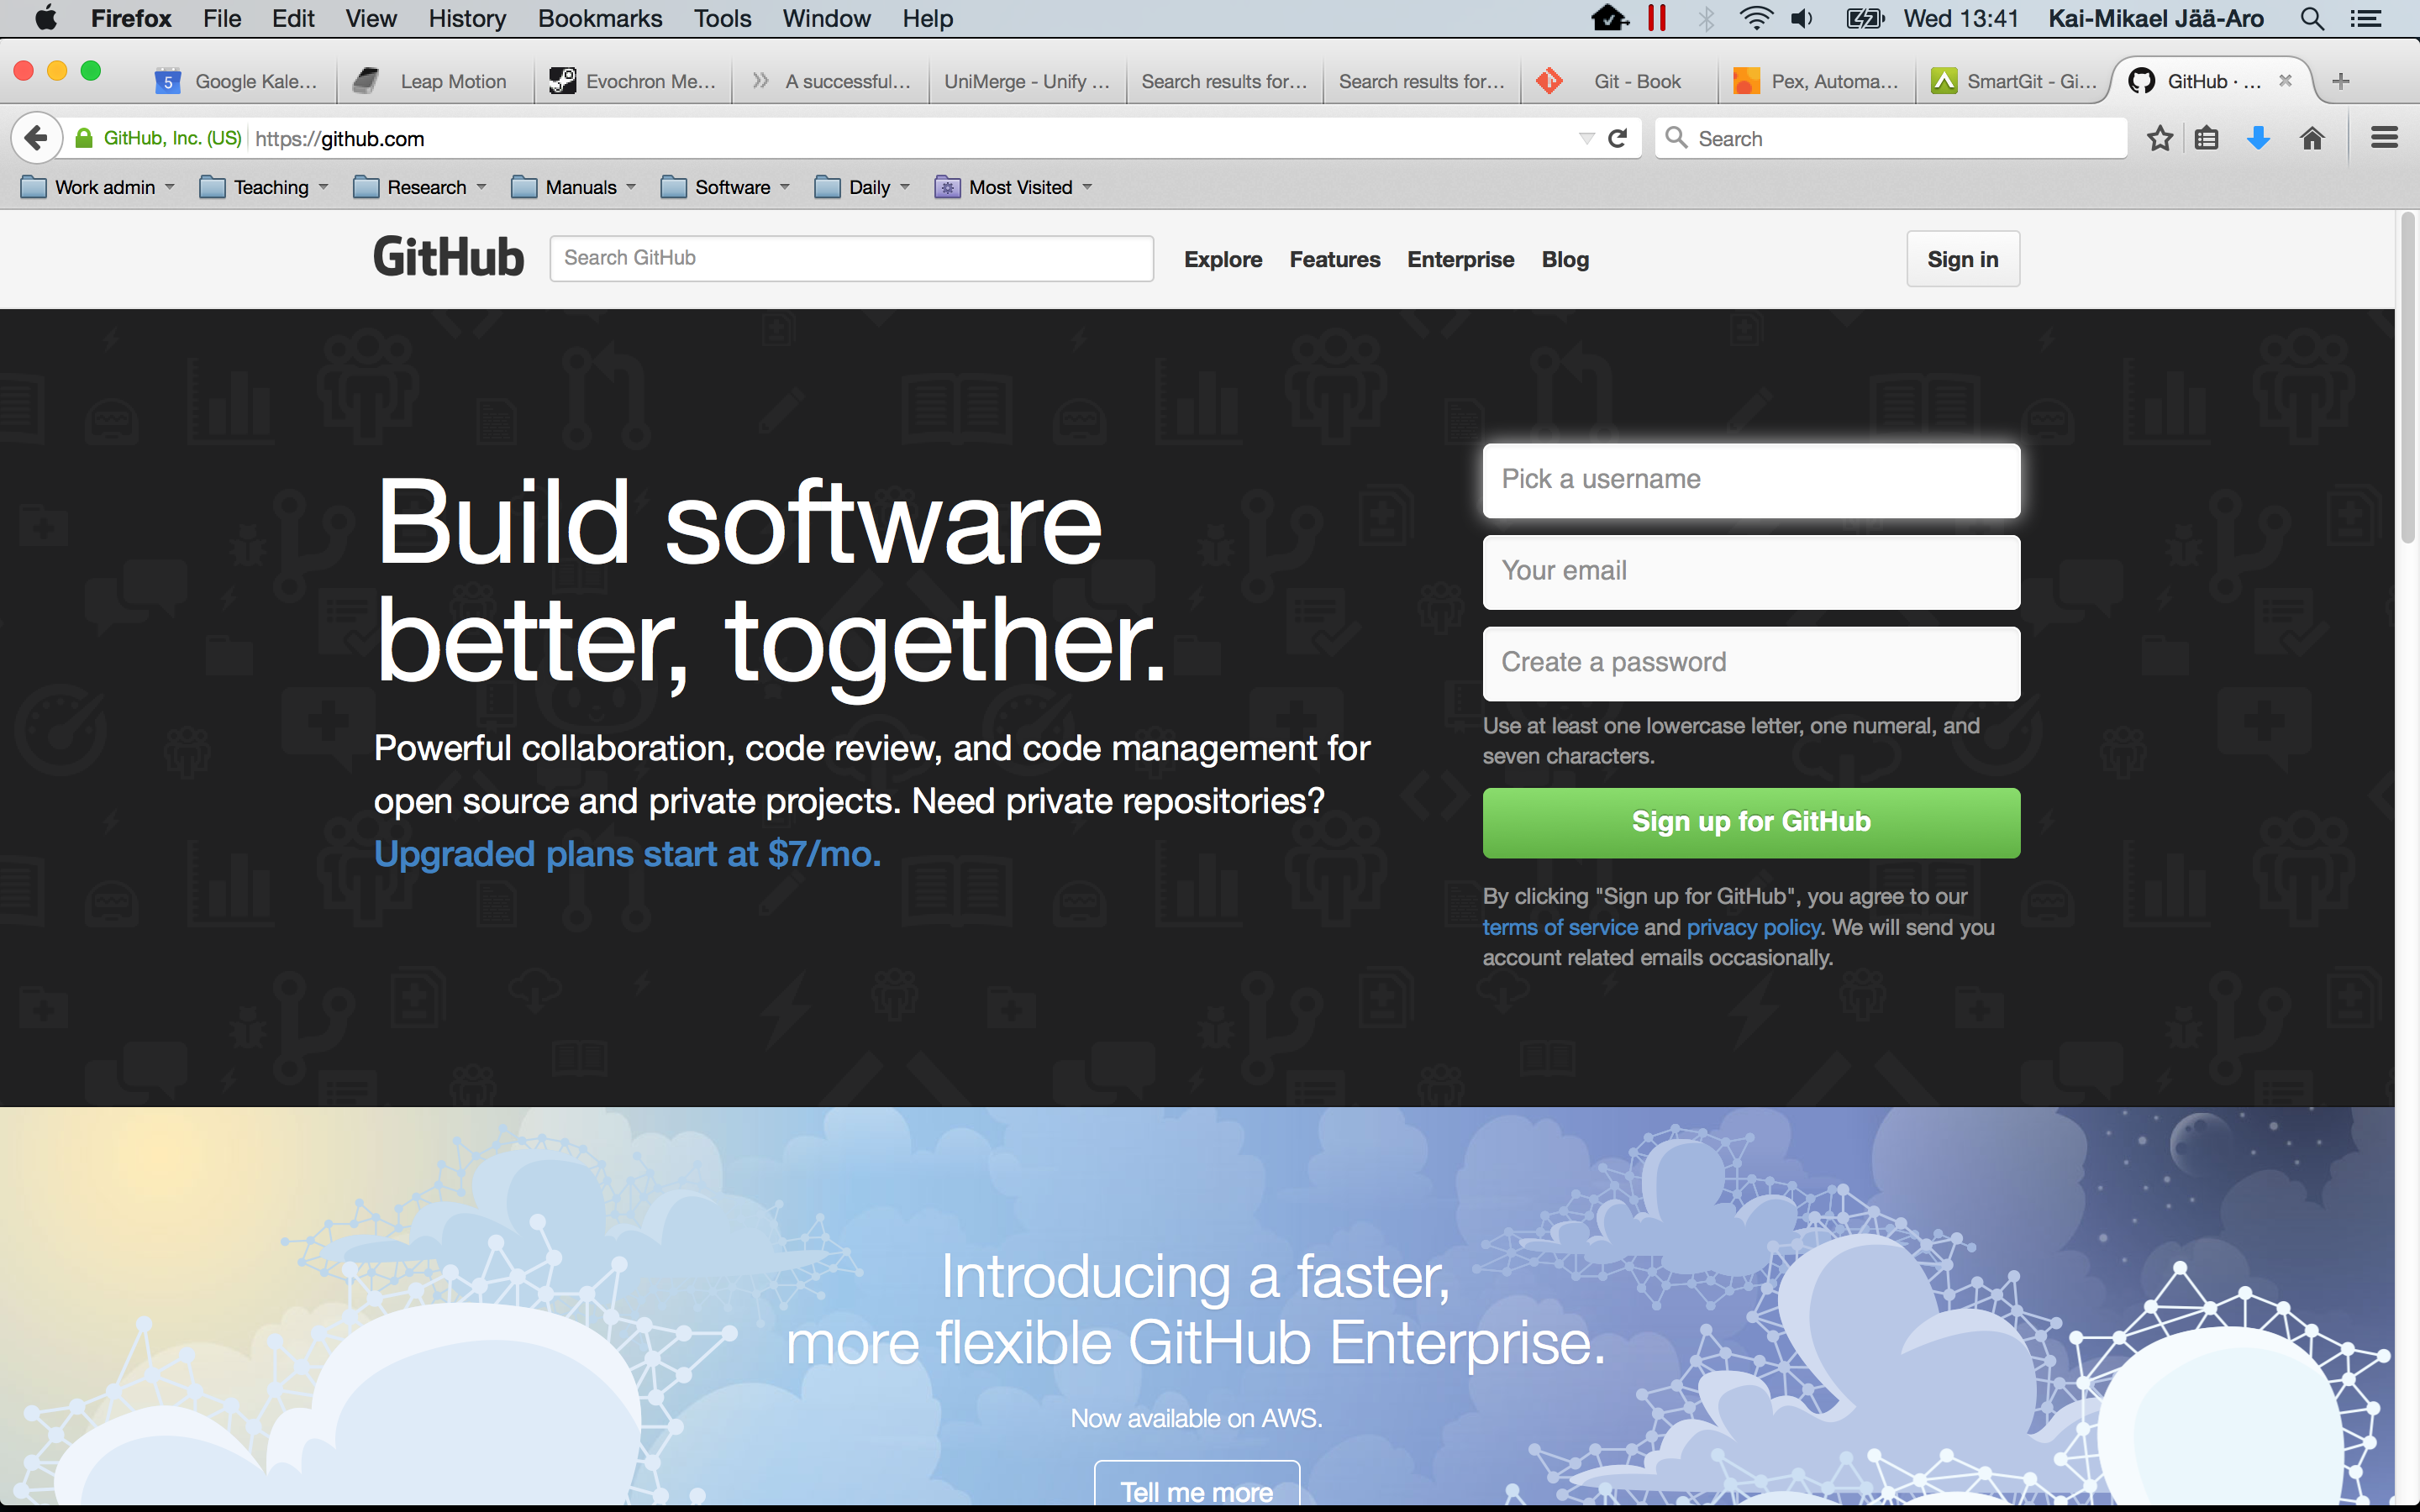
\includegraphics{GitHubSignUp}
\end{frame}

\begin{frame}
\frametitle{Välj funktioner/kostnadsnivå}
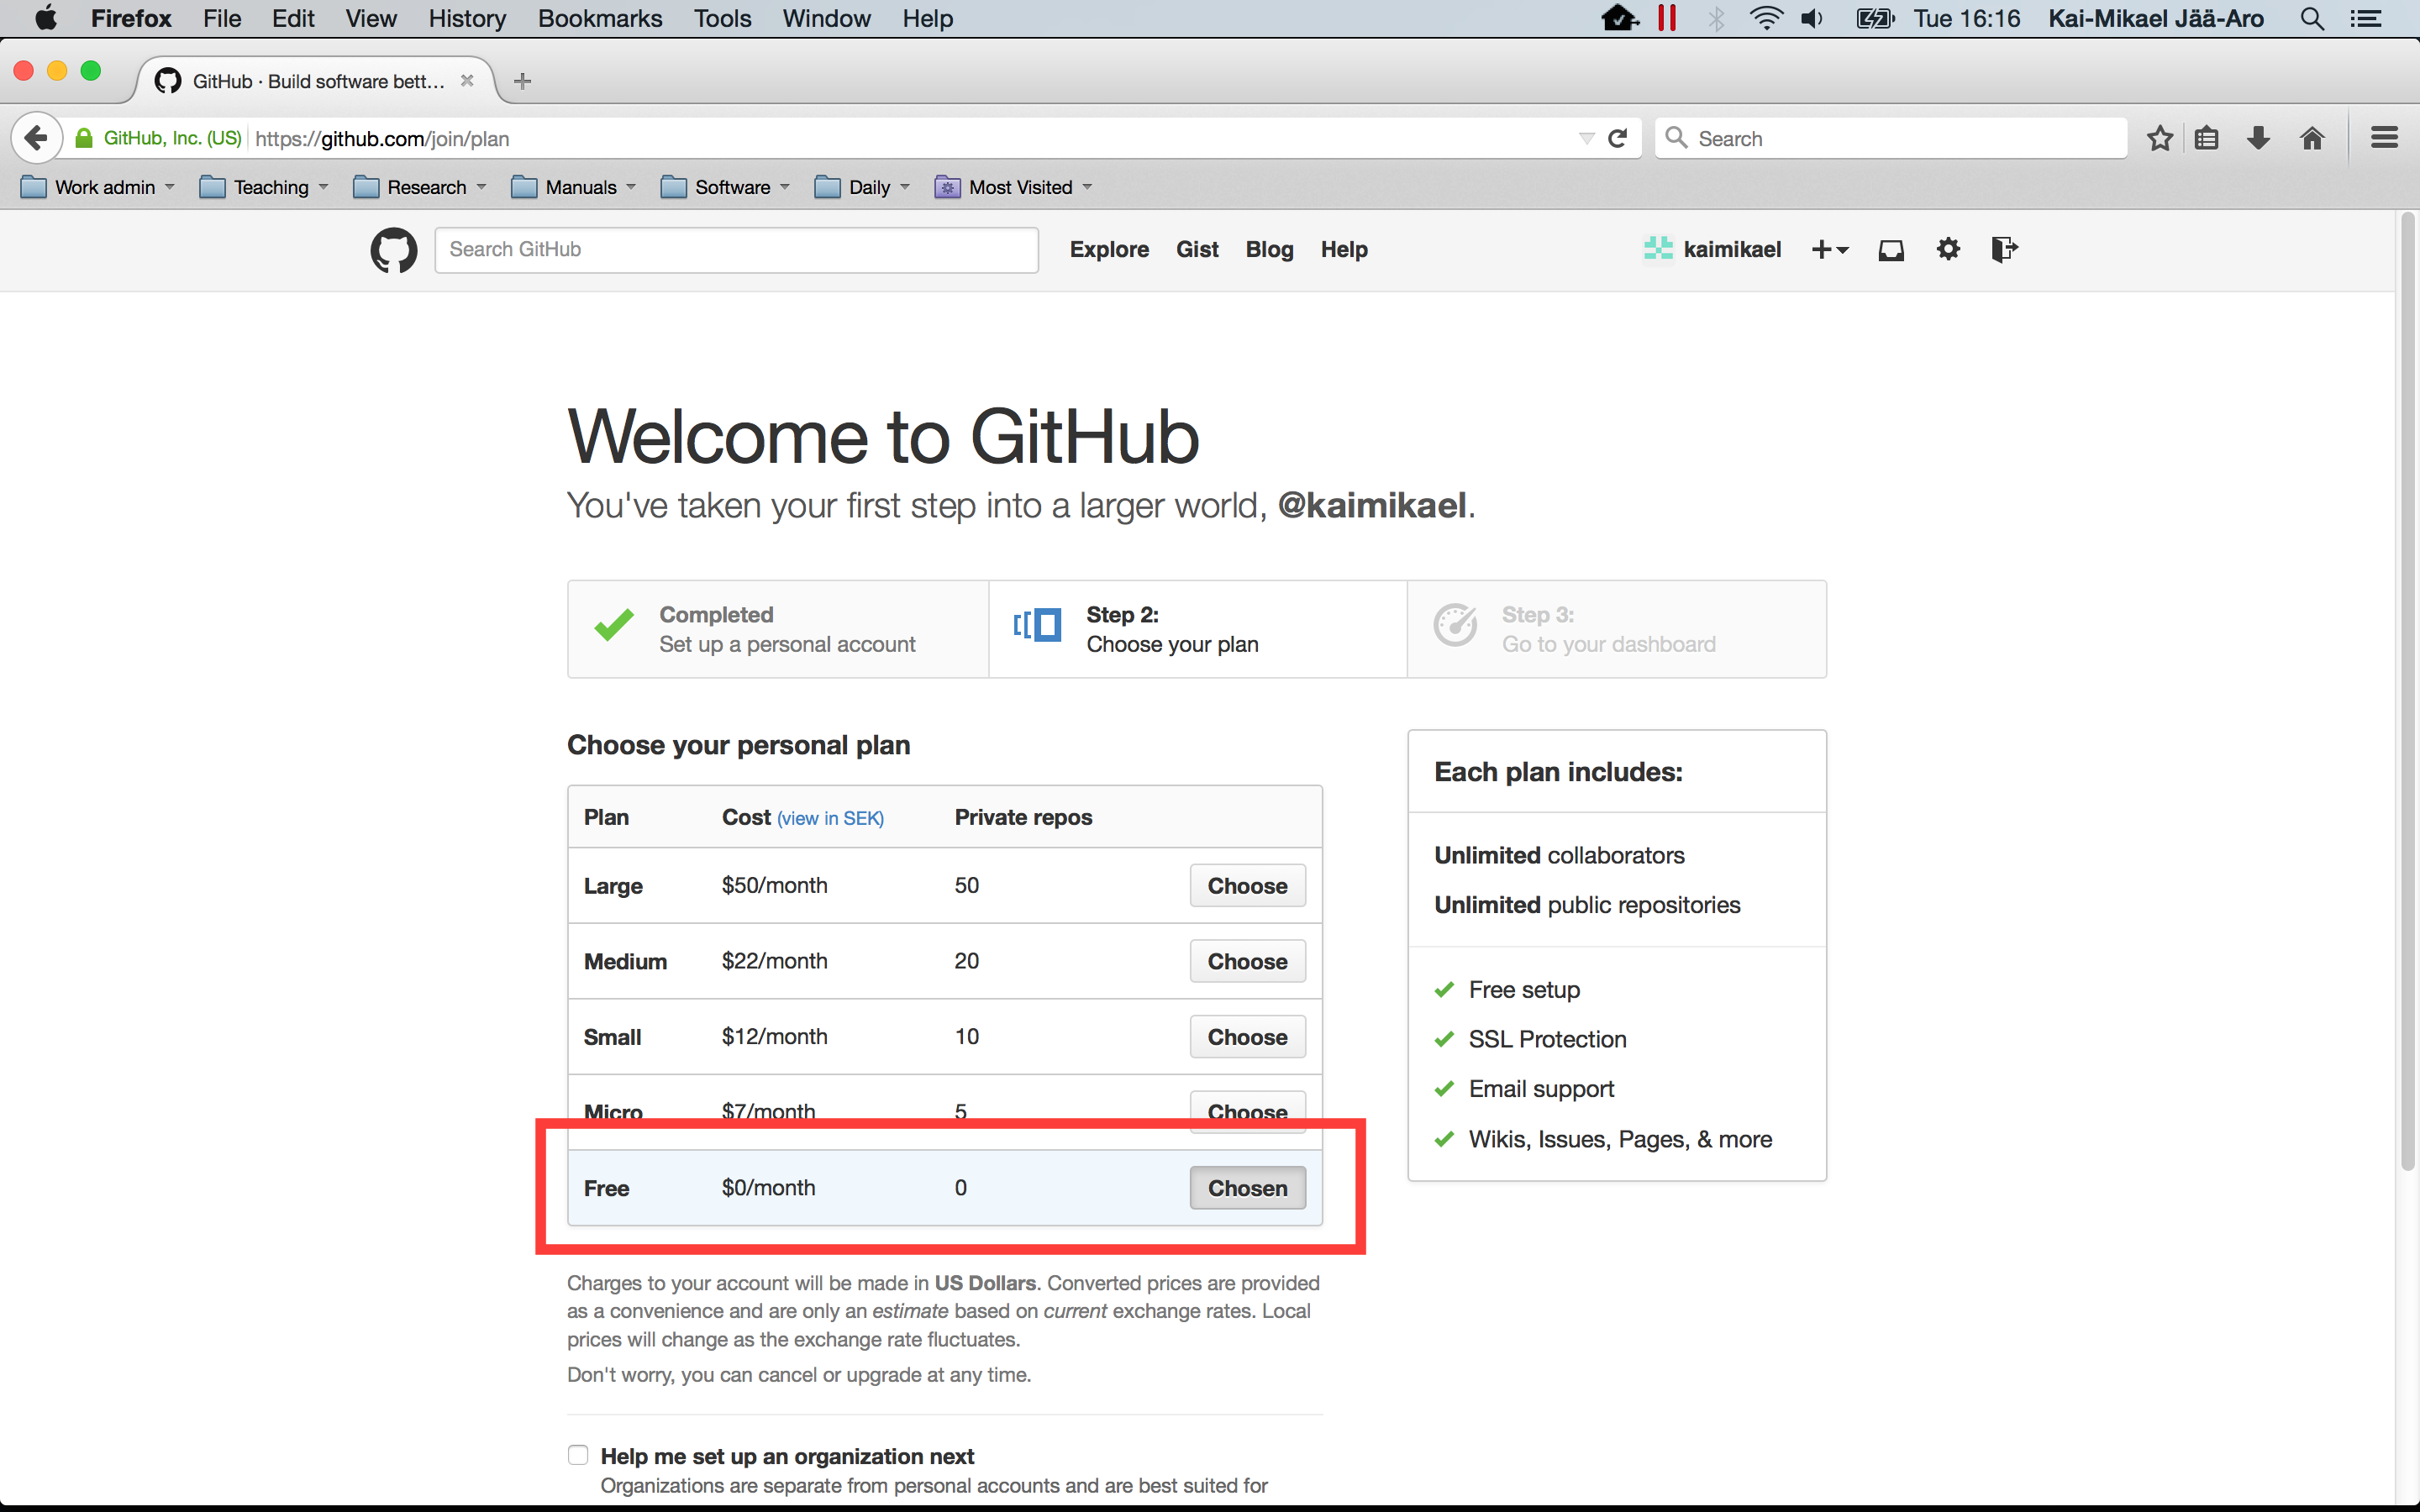
\includegraphics{GitHubChoosePlan}
\end{frame}


\begin{frame}
\frametitle{Skapa ett arkiv}
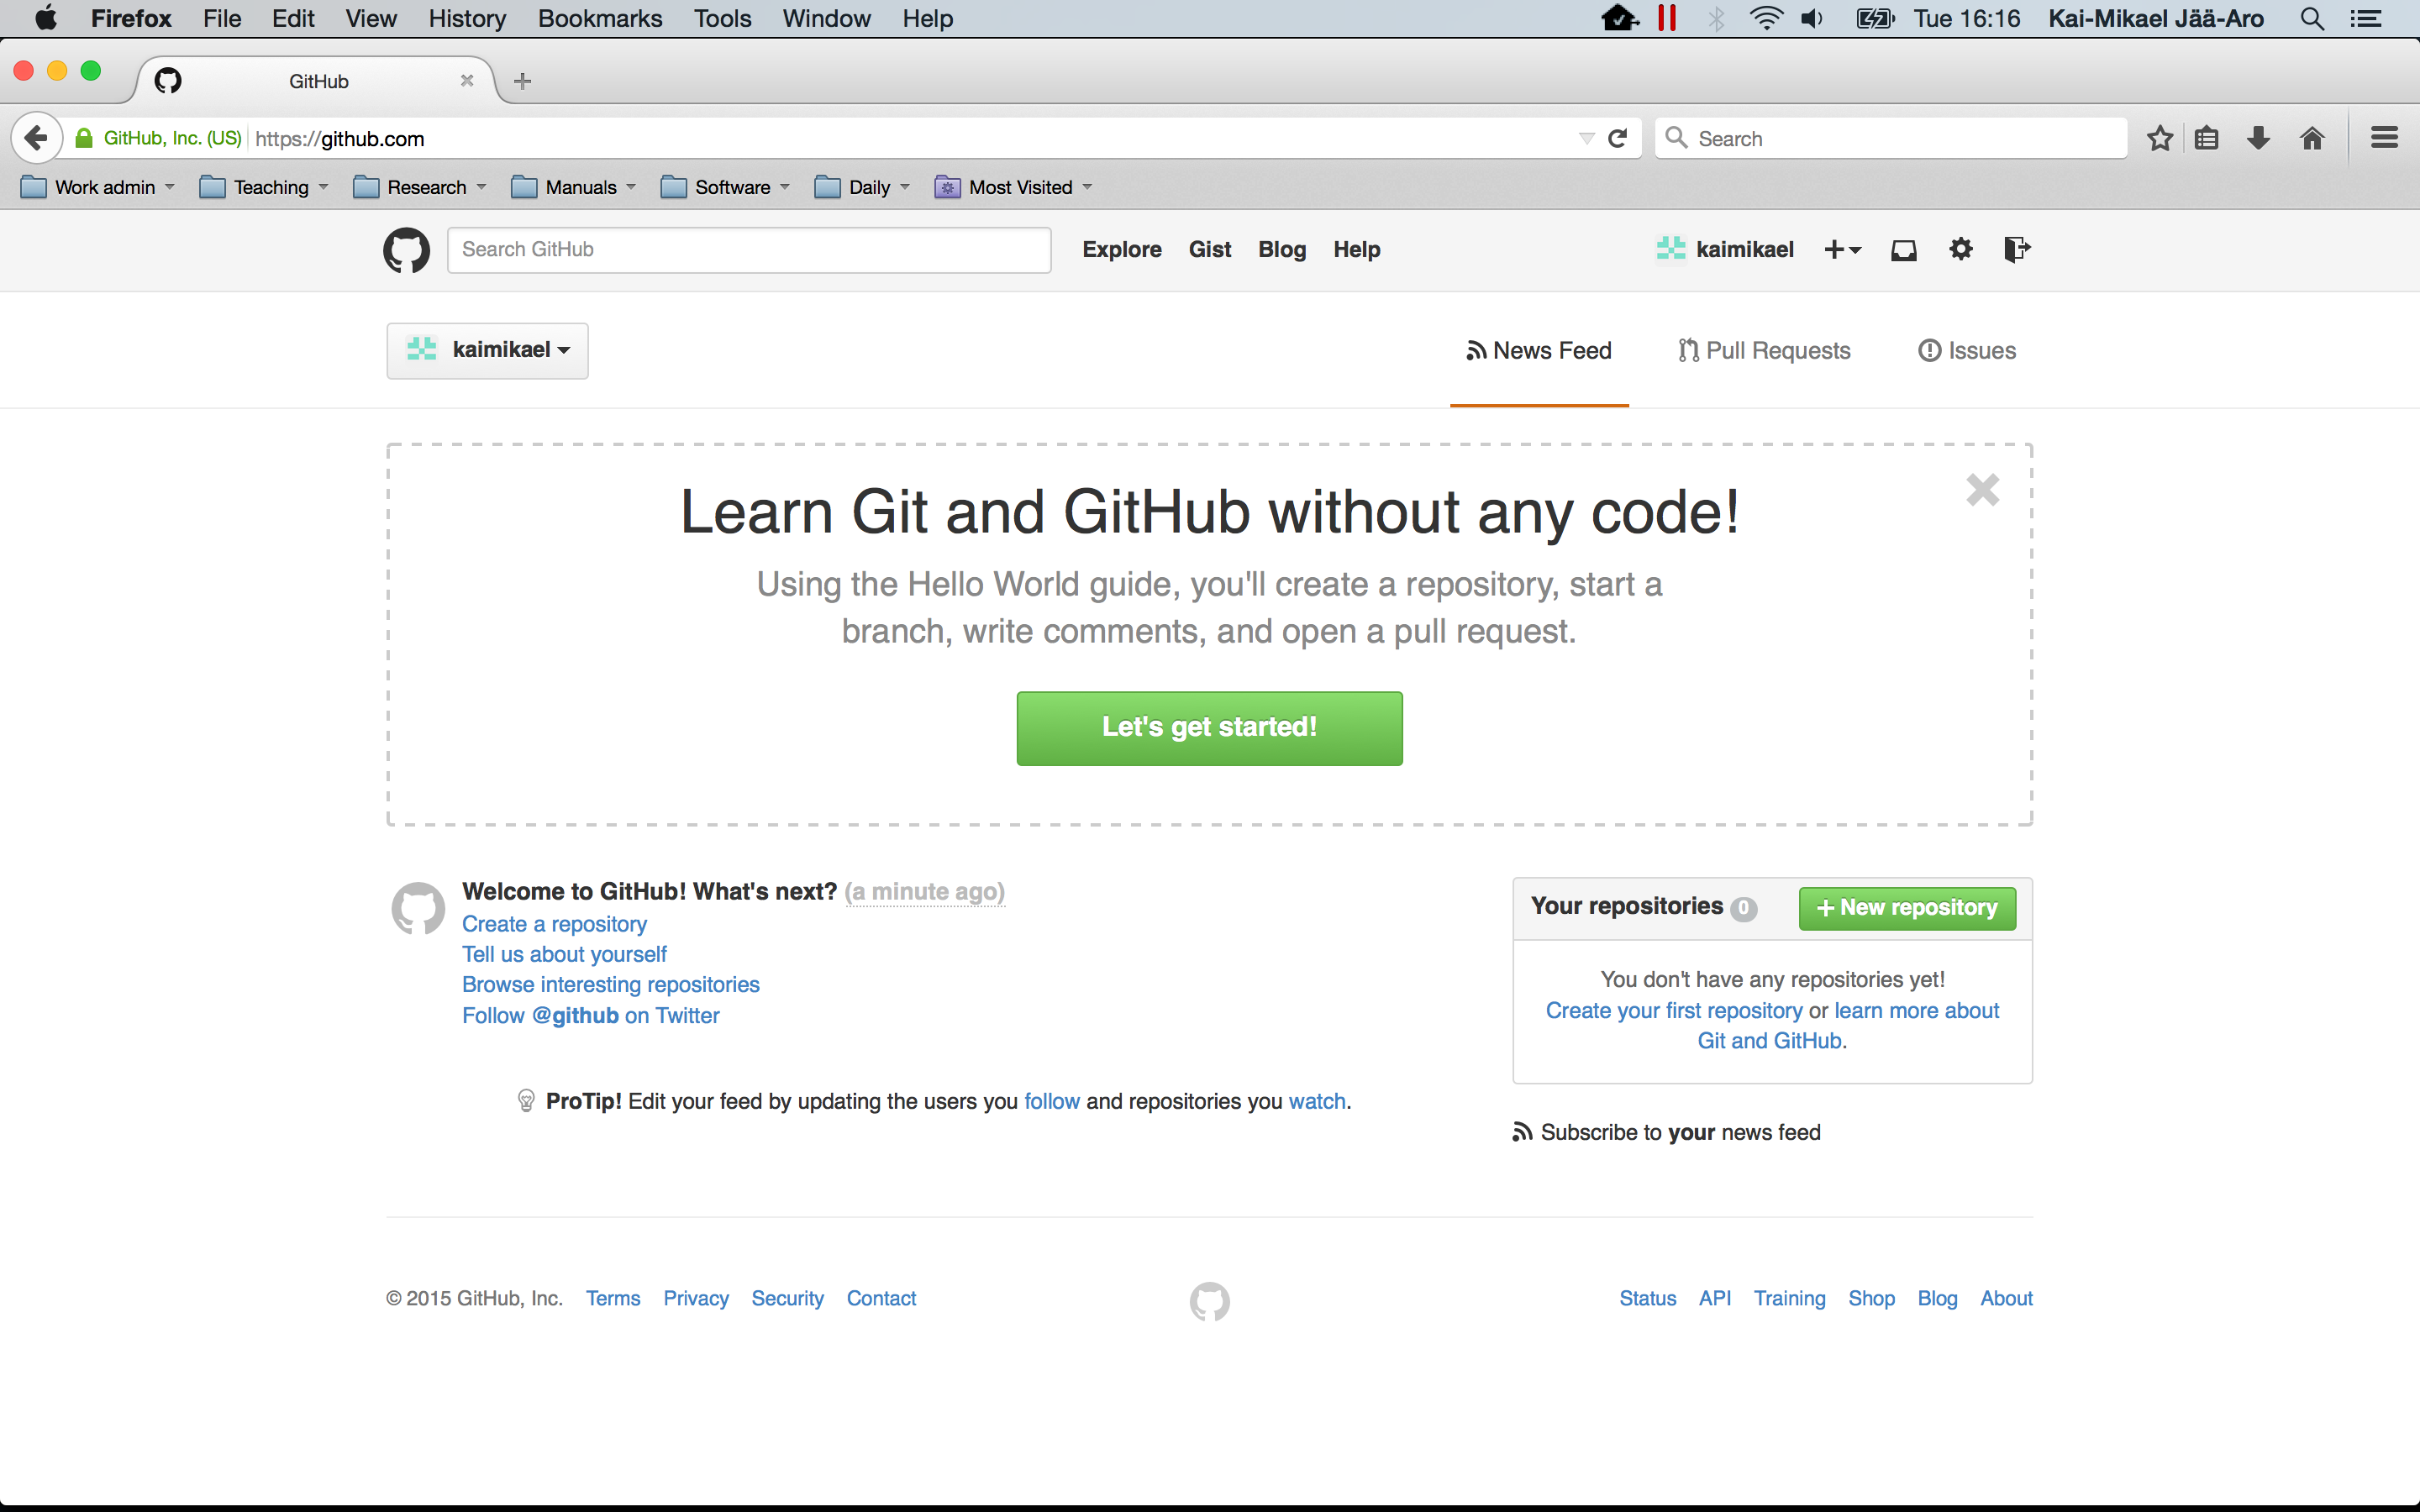
\includegraphics{GitHubCreateRepository}  
\end{frame}

\begin{frame}
\frametitle{Konfigurera arkivet}
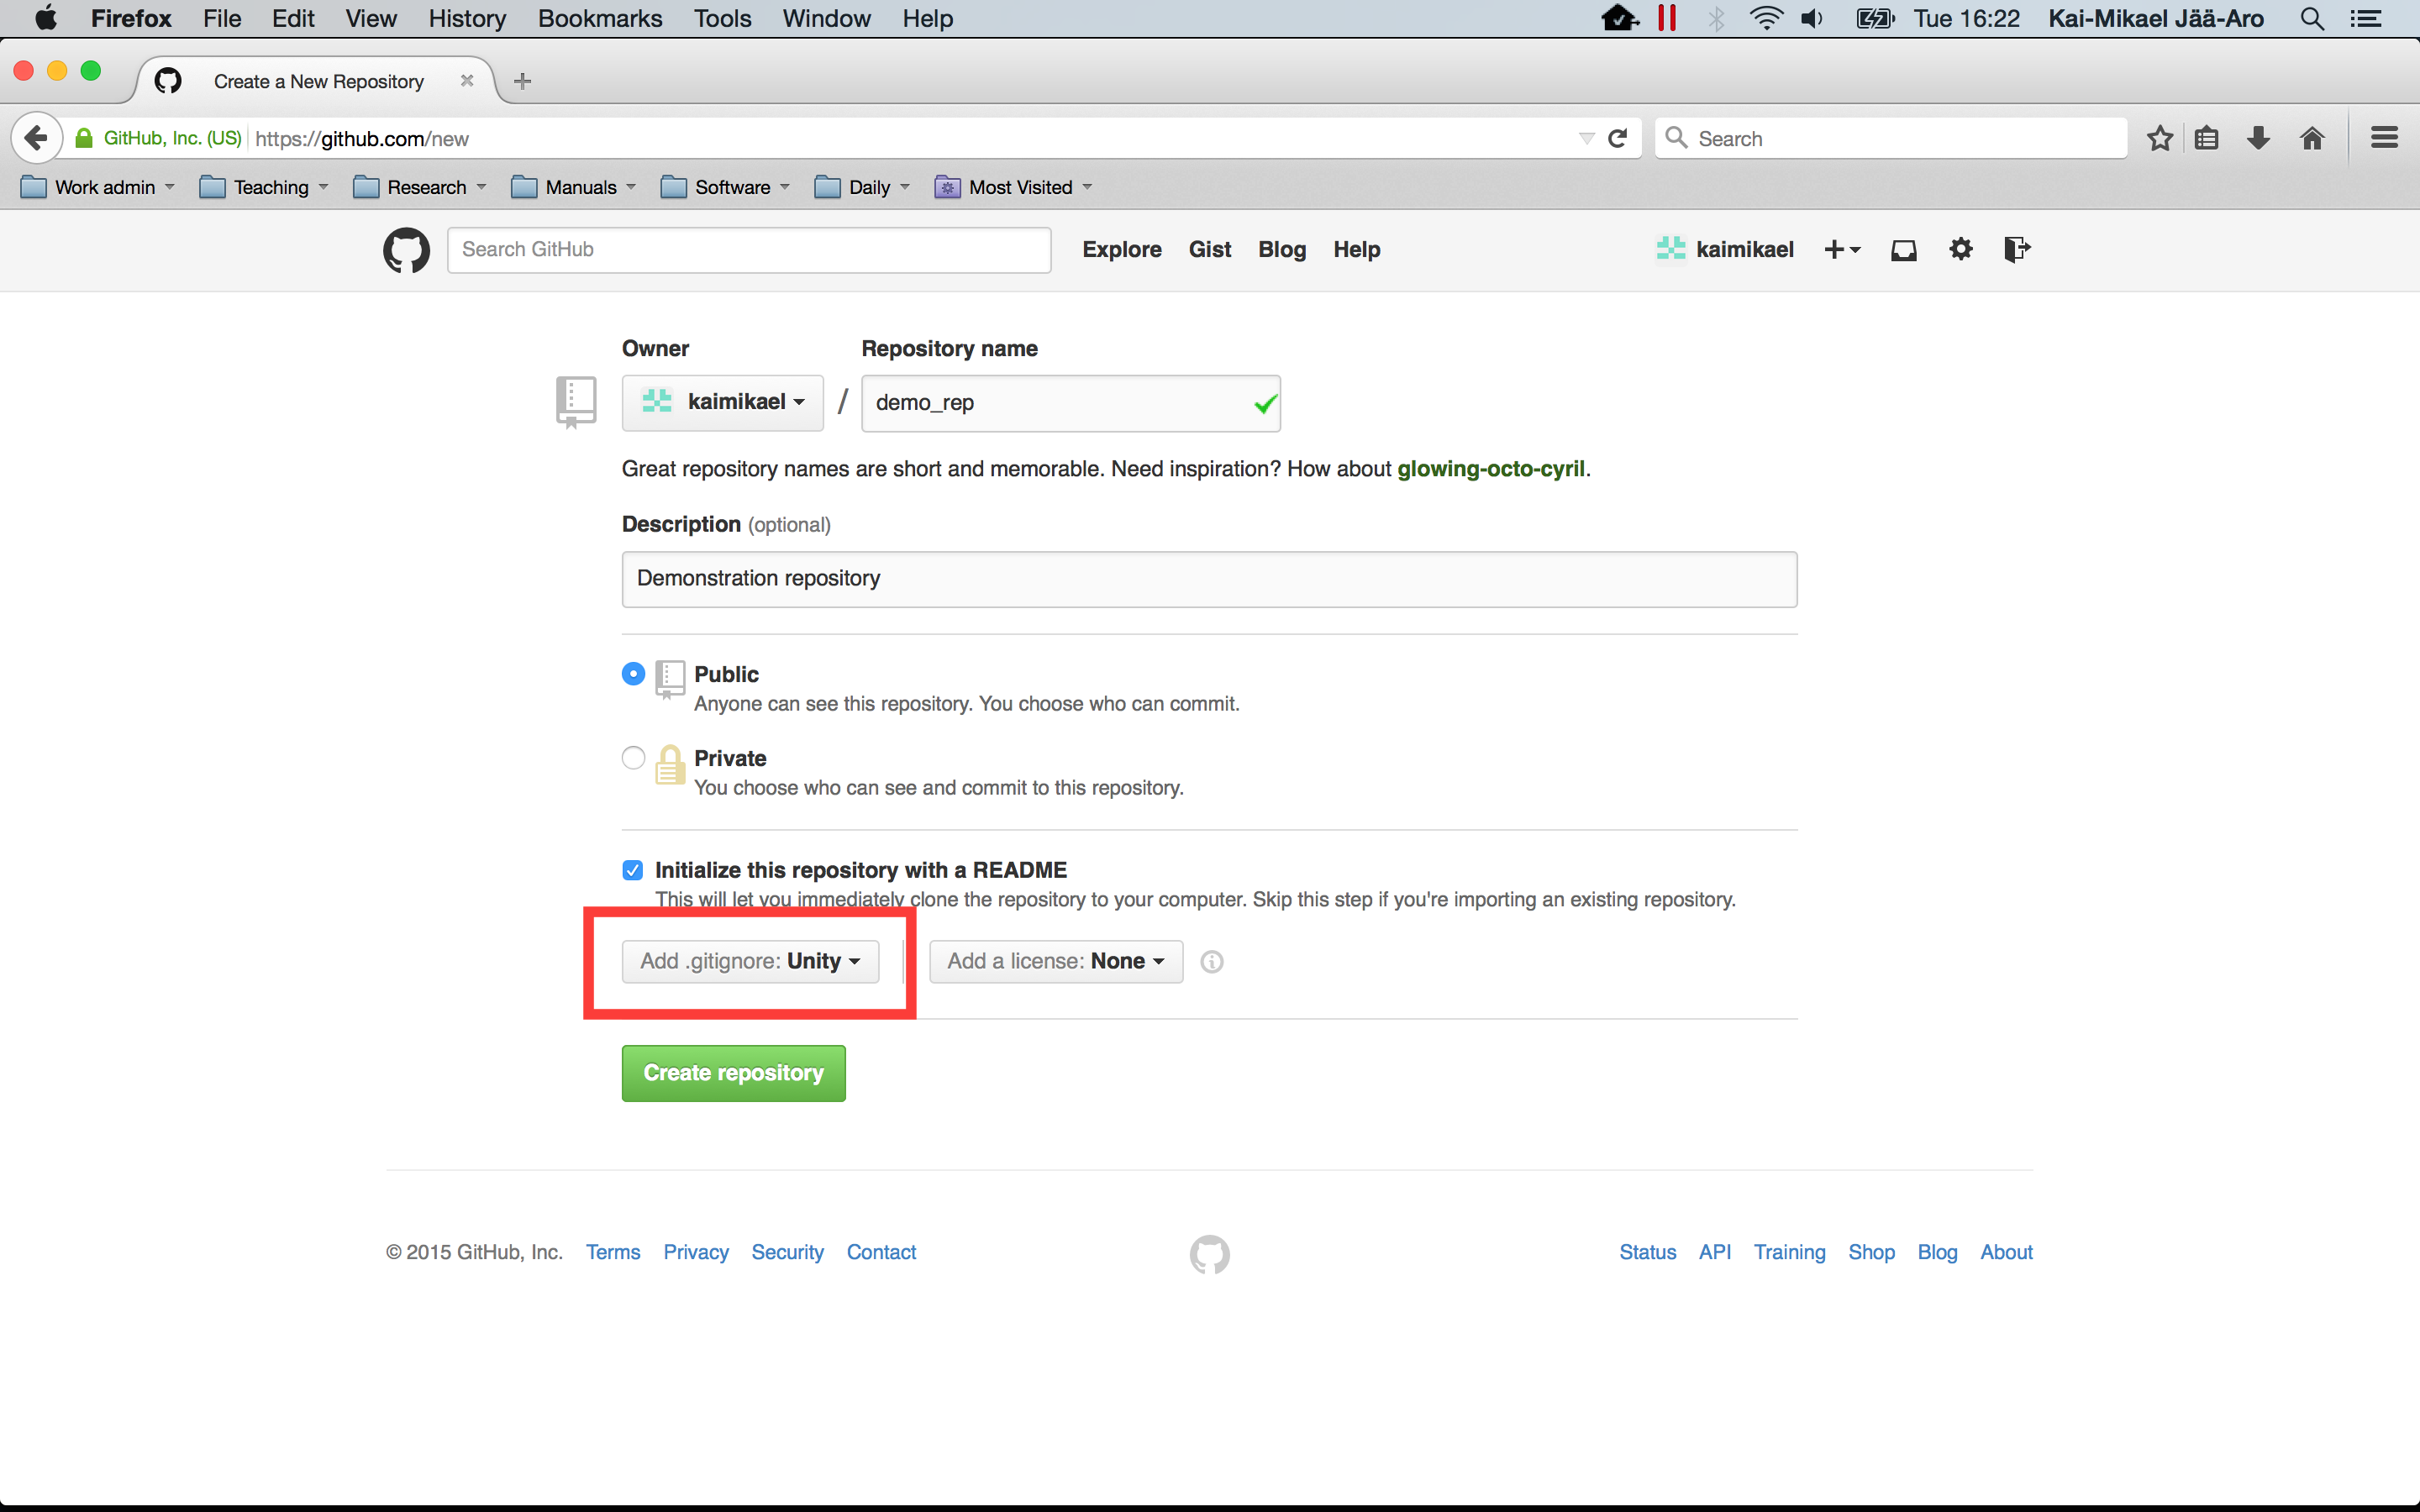
\includegraphics{GitHubNameRepository}
\end{frame}

\begin{frame}
\frametitle{Lägg till medarbetare}
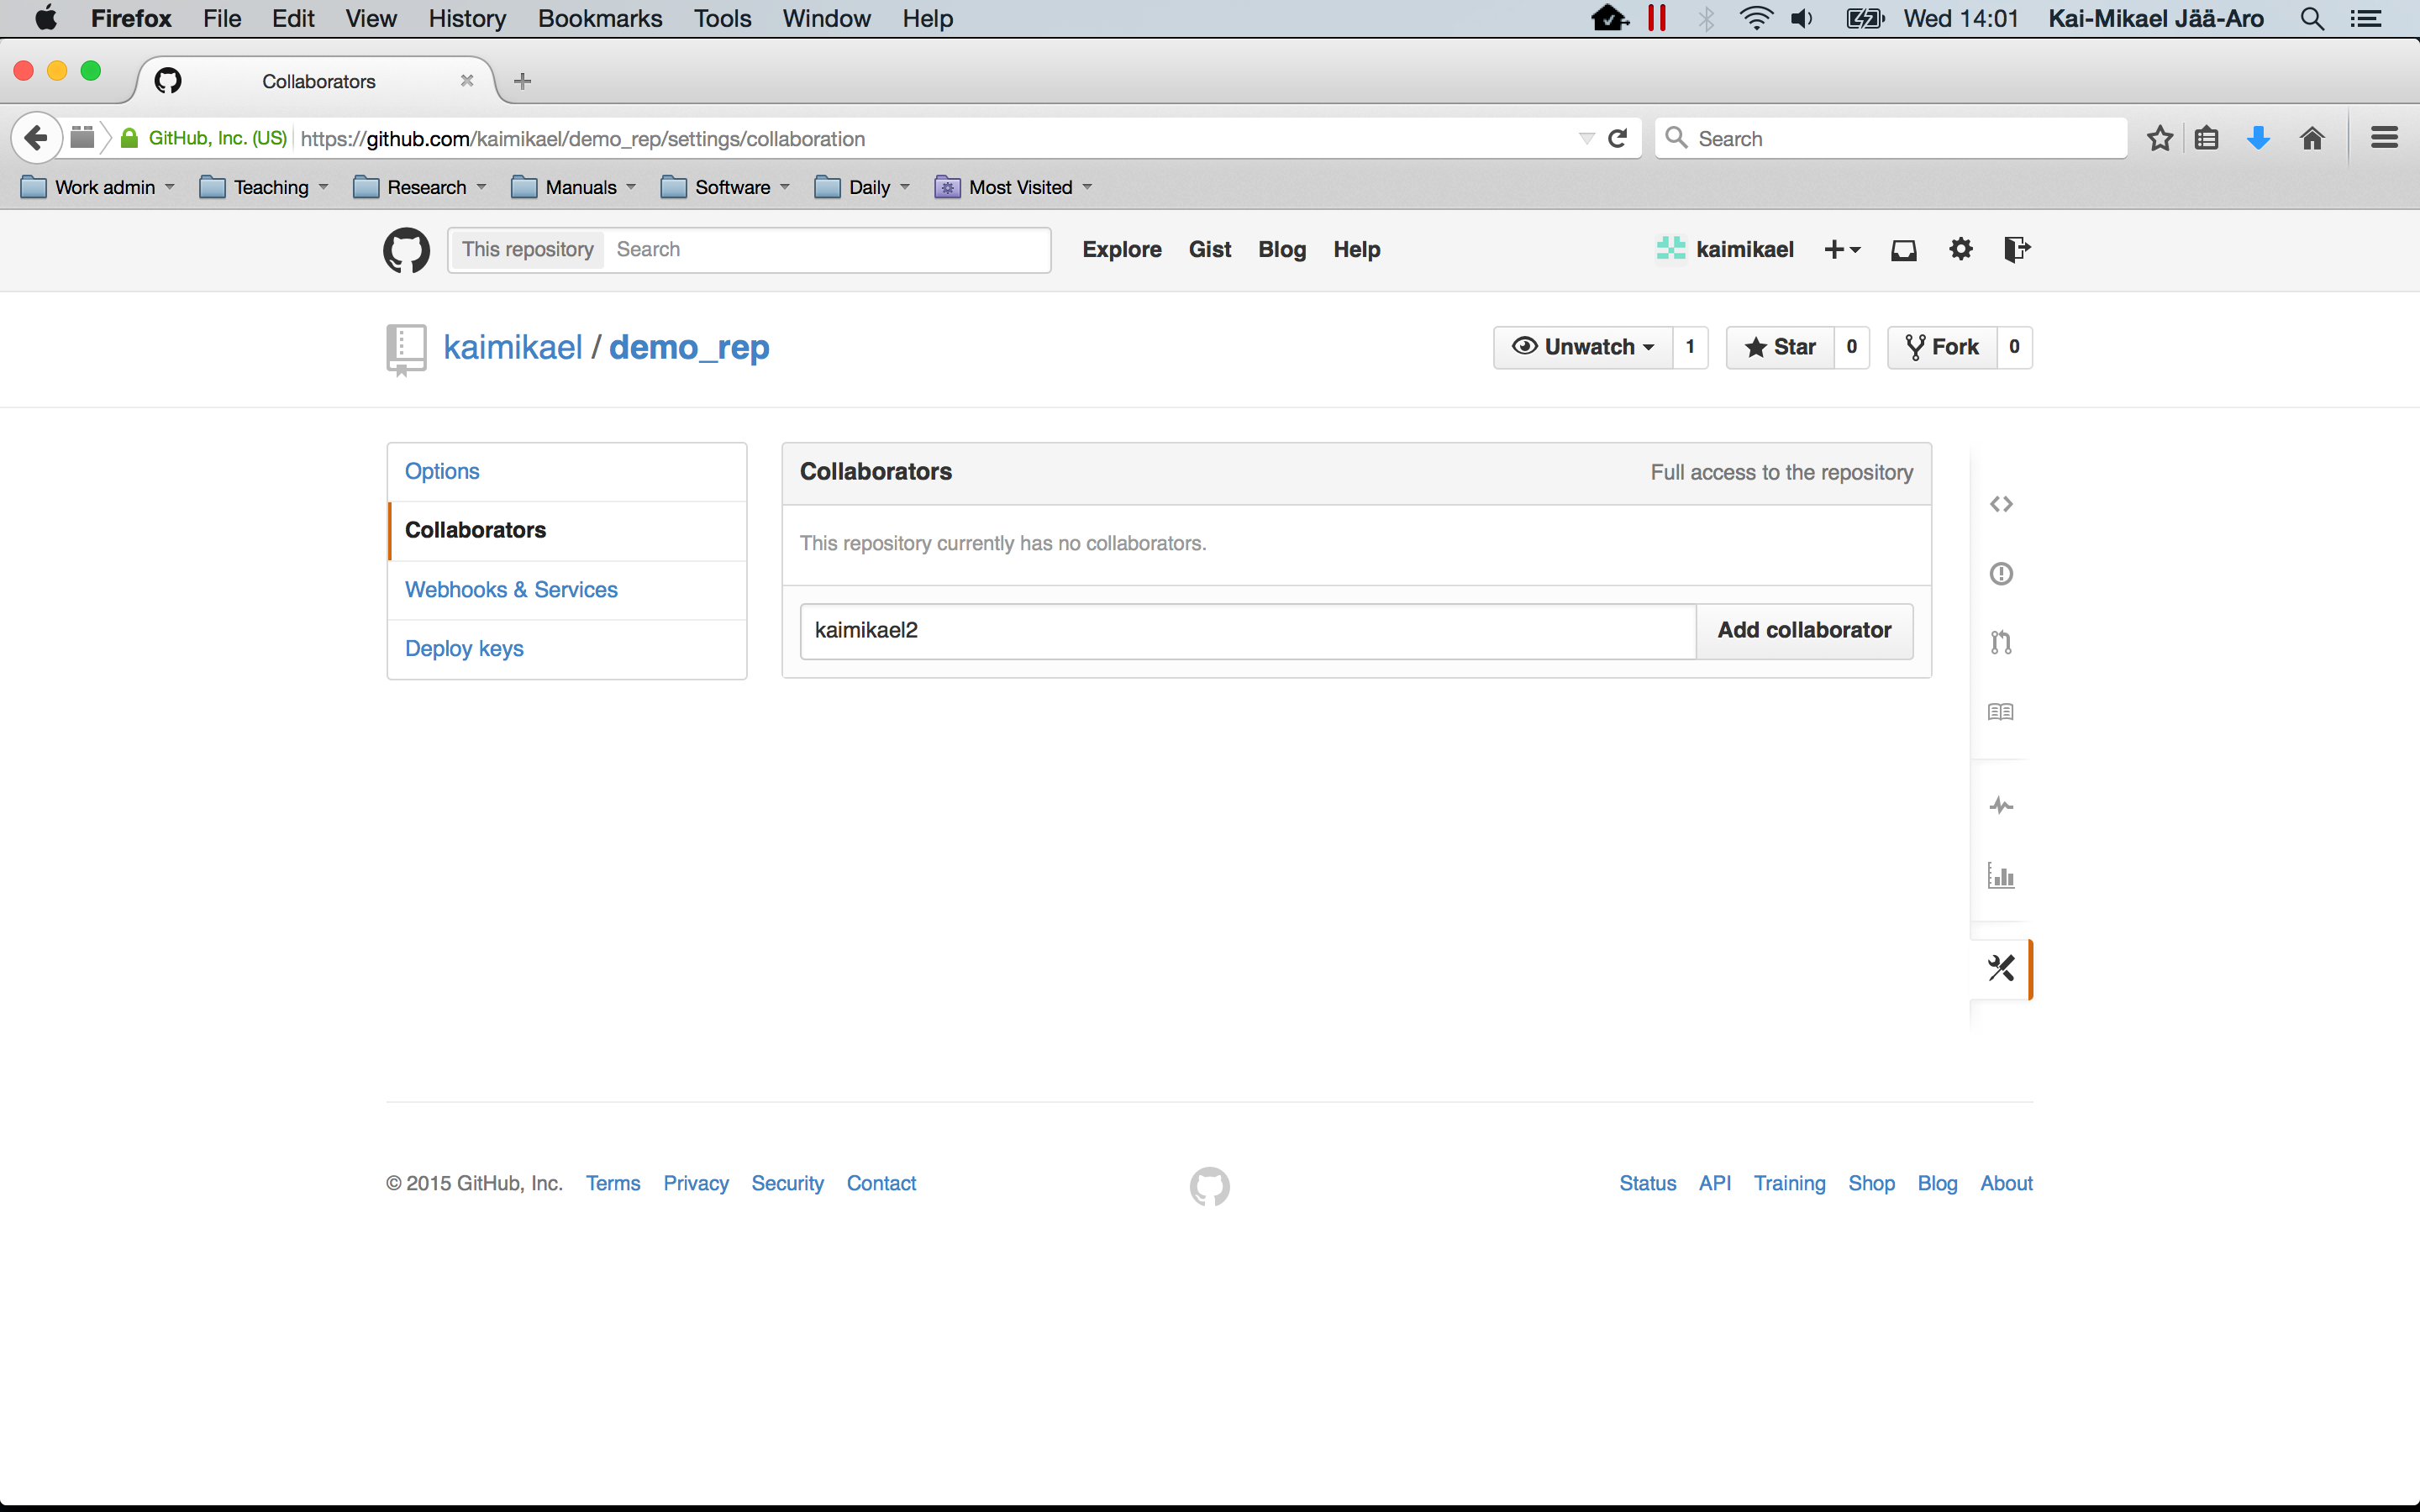
\includegraphics{GitHubAddCollaborators}
\end{frame}

\begin{frame}
\frametitle{Gör en lokal arkiv-klon}
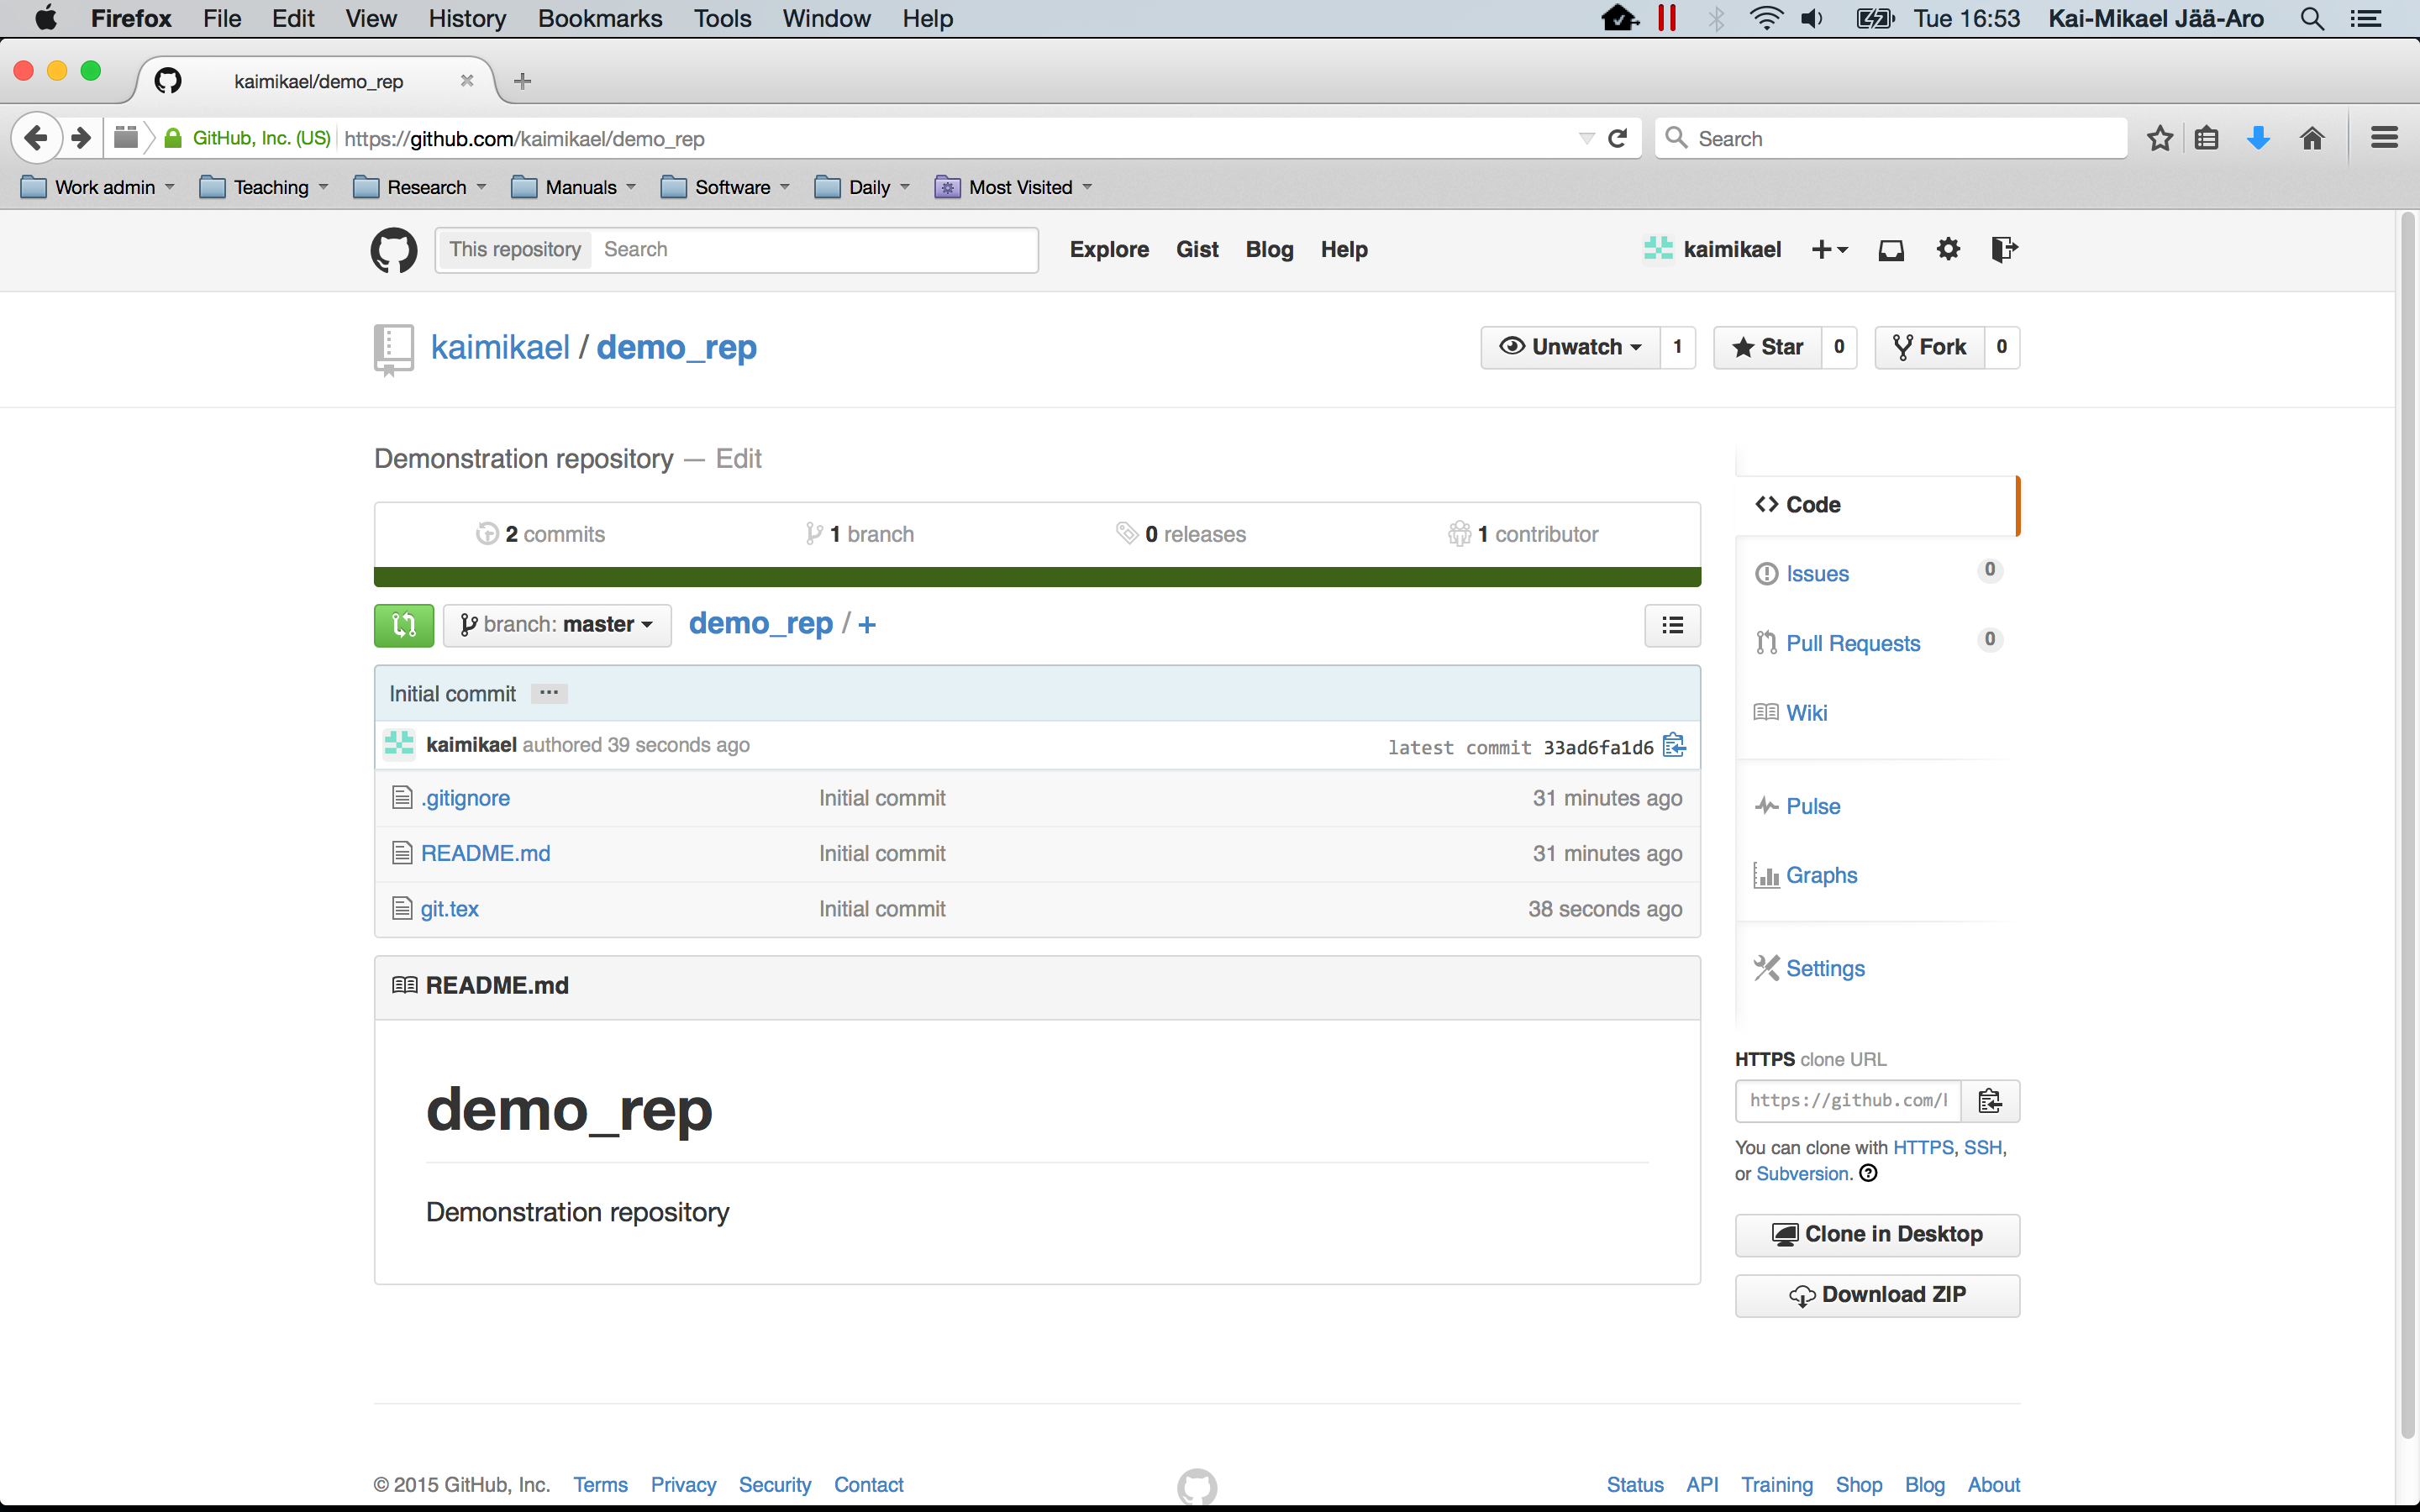
\includegraphics{GitHubWebInterface}
\end{frame}

\subsection{GitHub-klienten}
\begin{frame}
\frametitle{Hämta klienten}
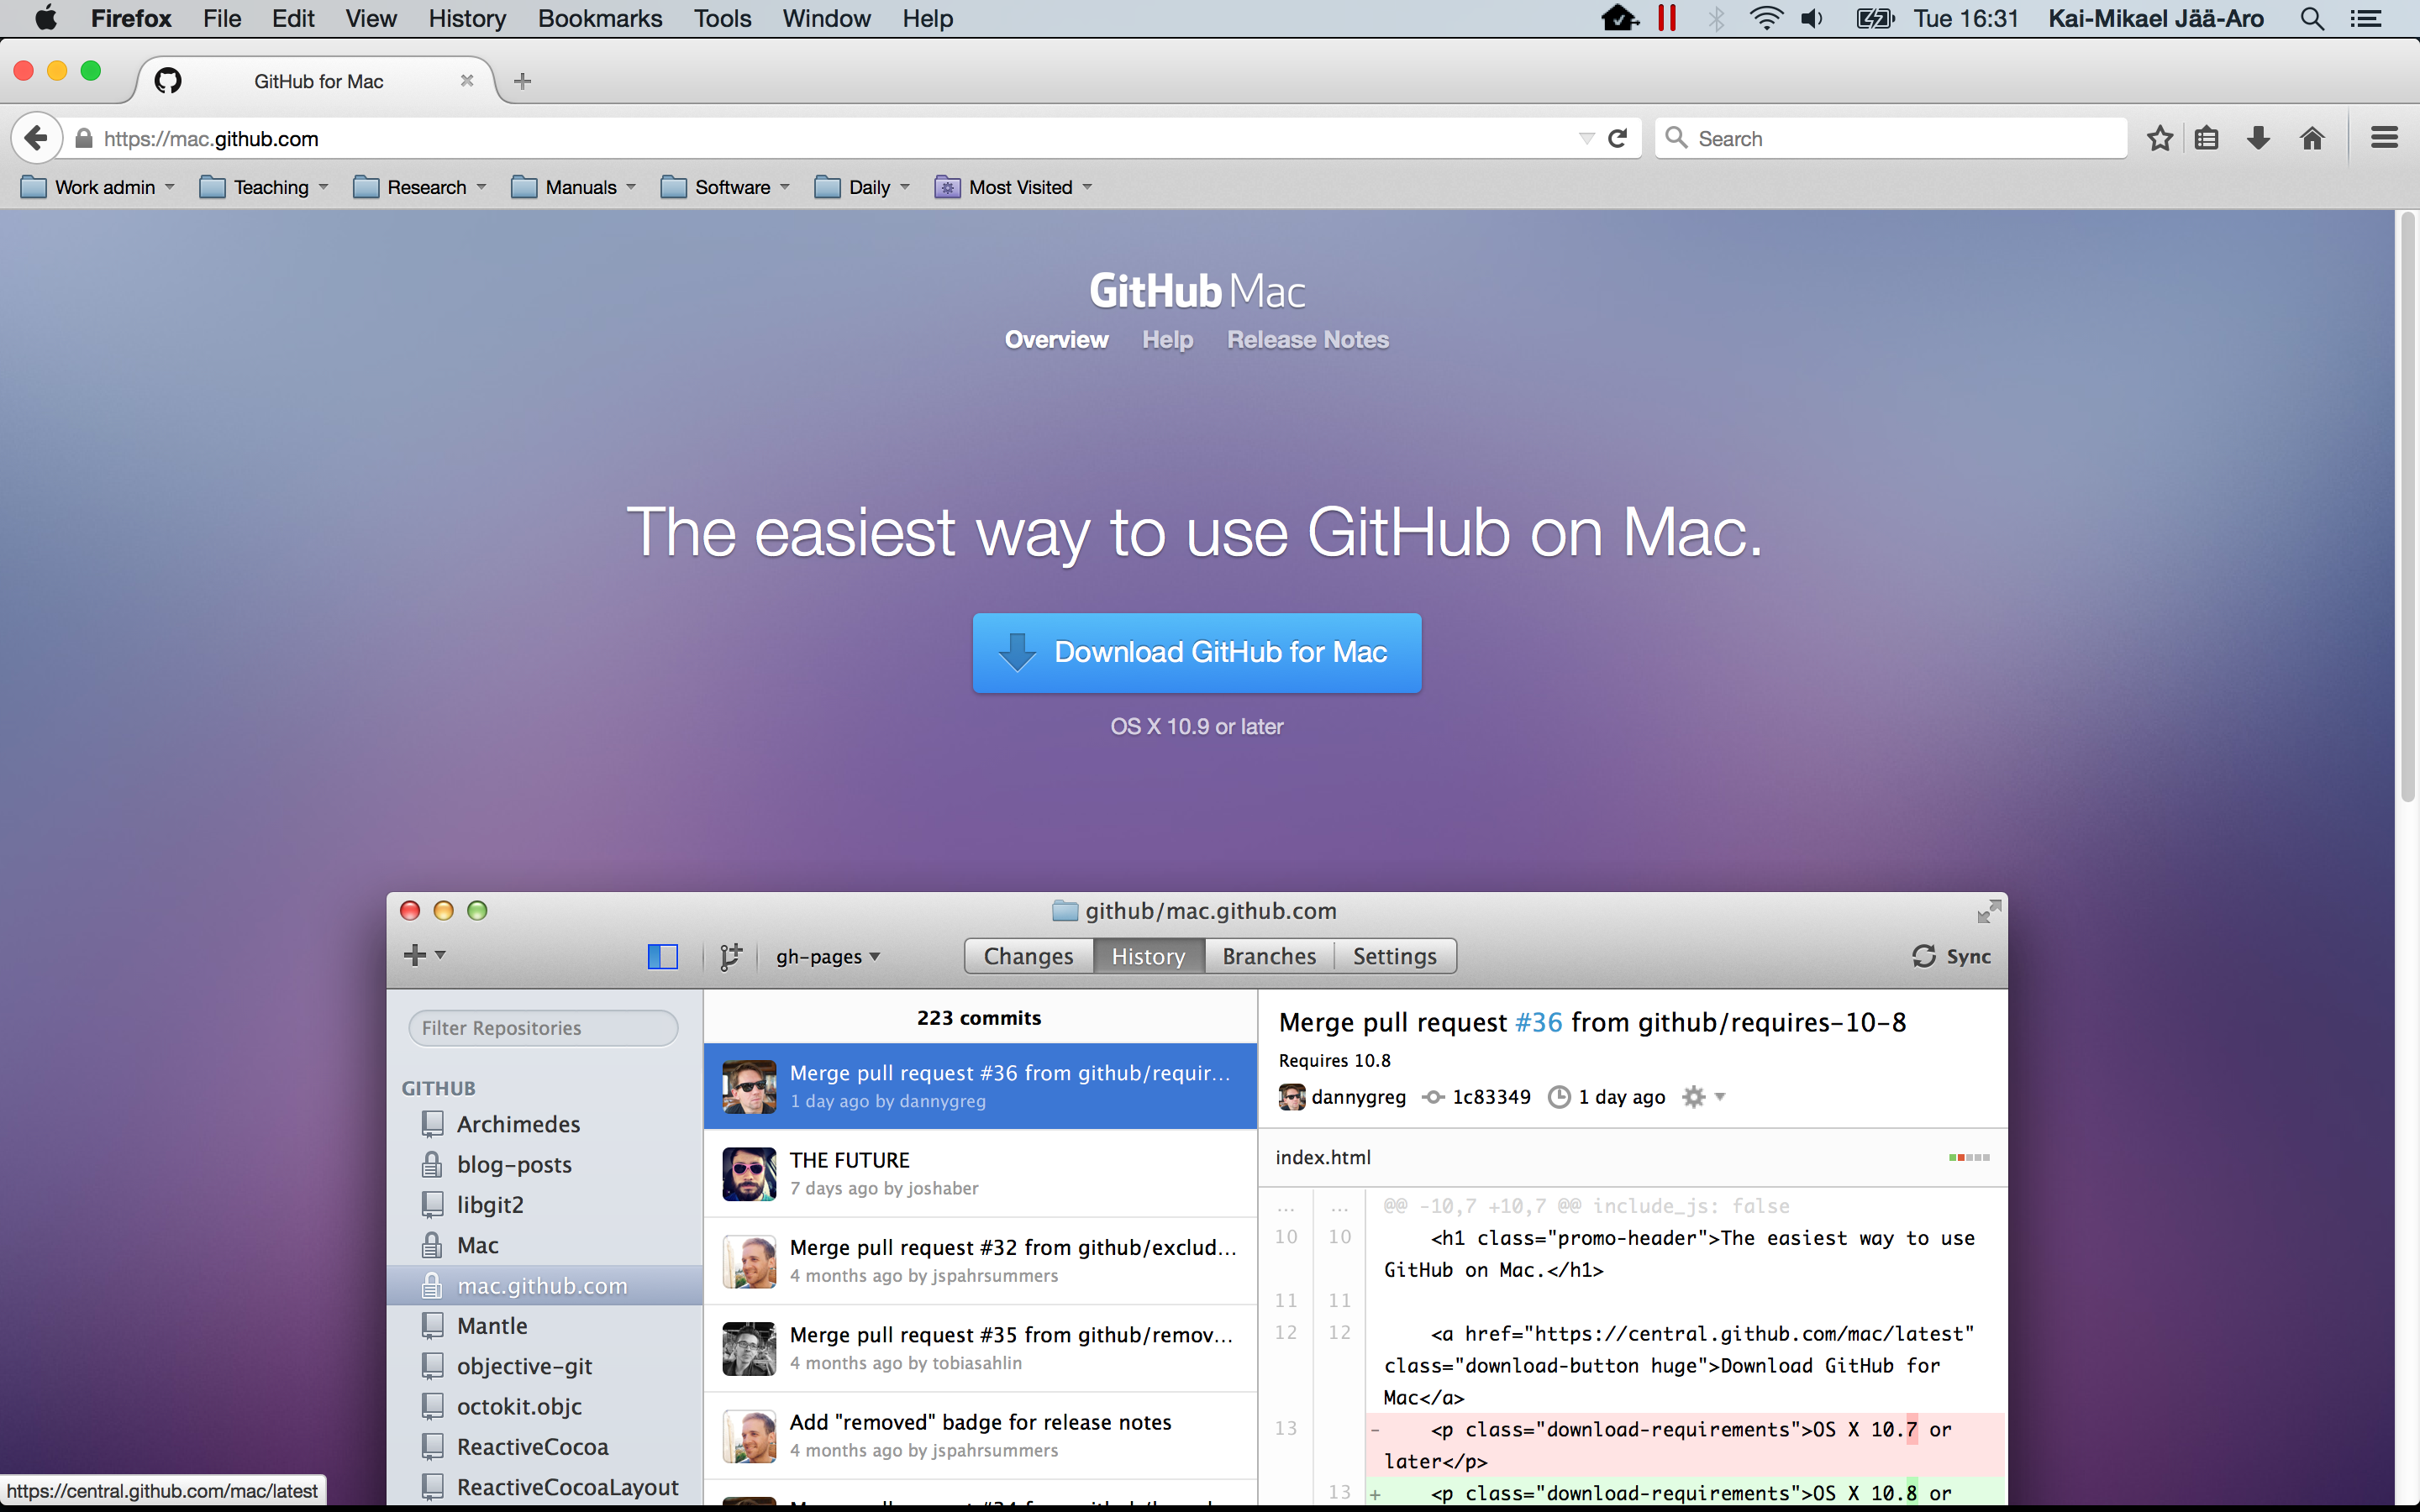
\includegraphics{GitHubDownload}

\end{frame}

\begin{frame}
\frametitle{Installera klienten}
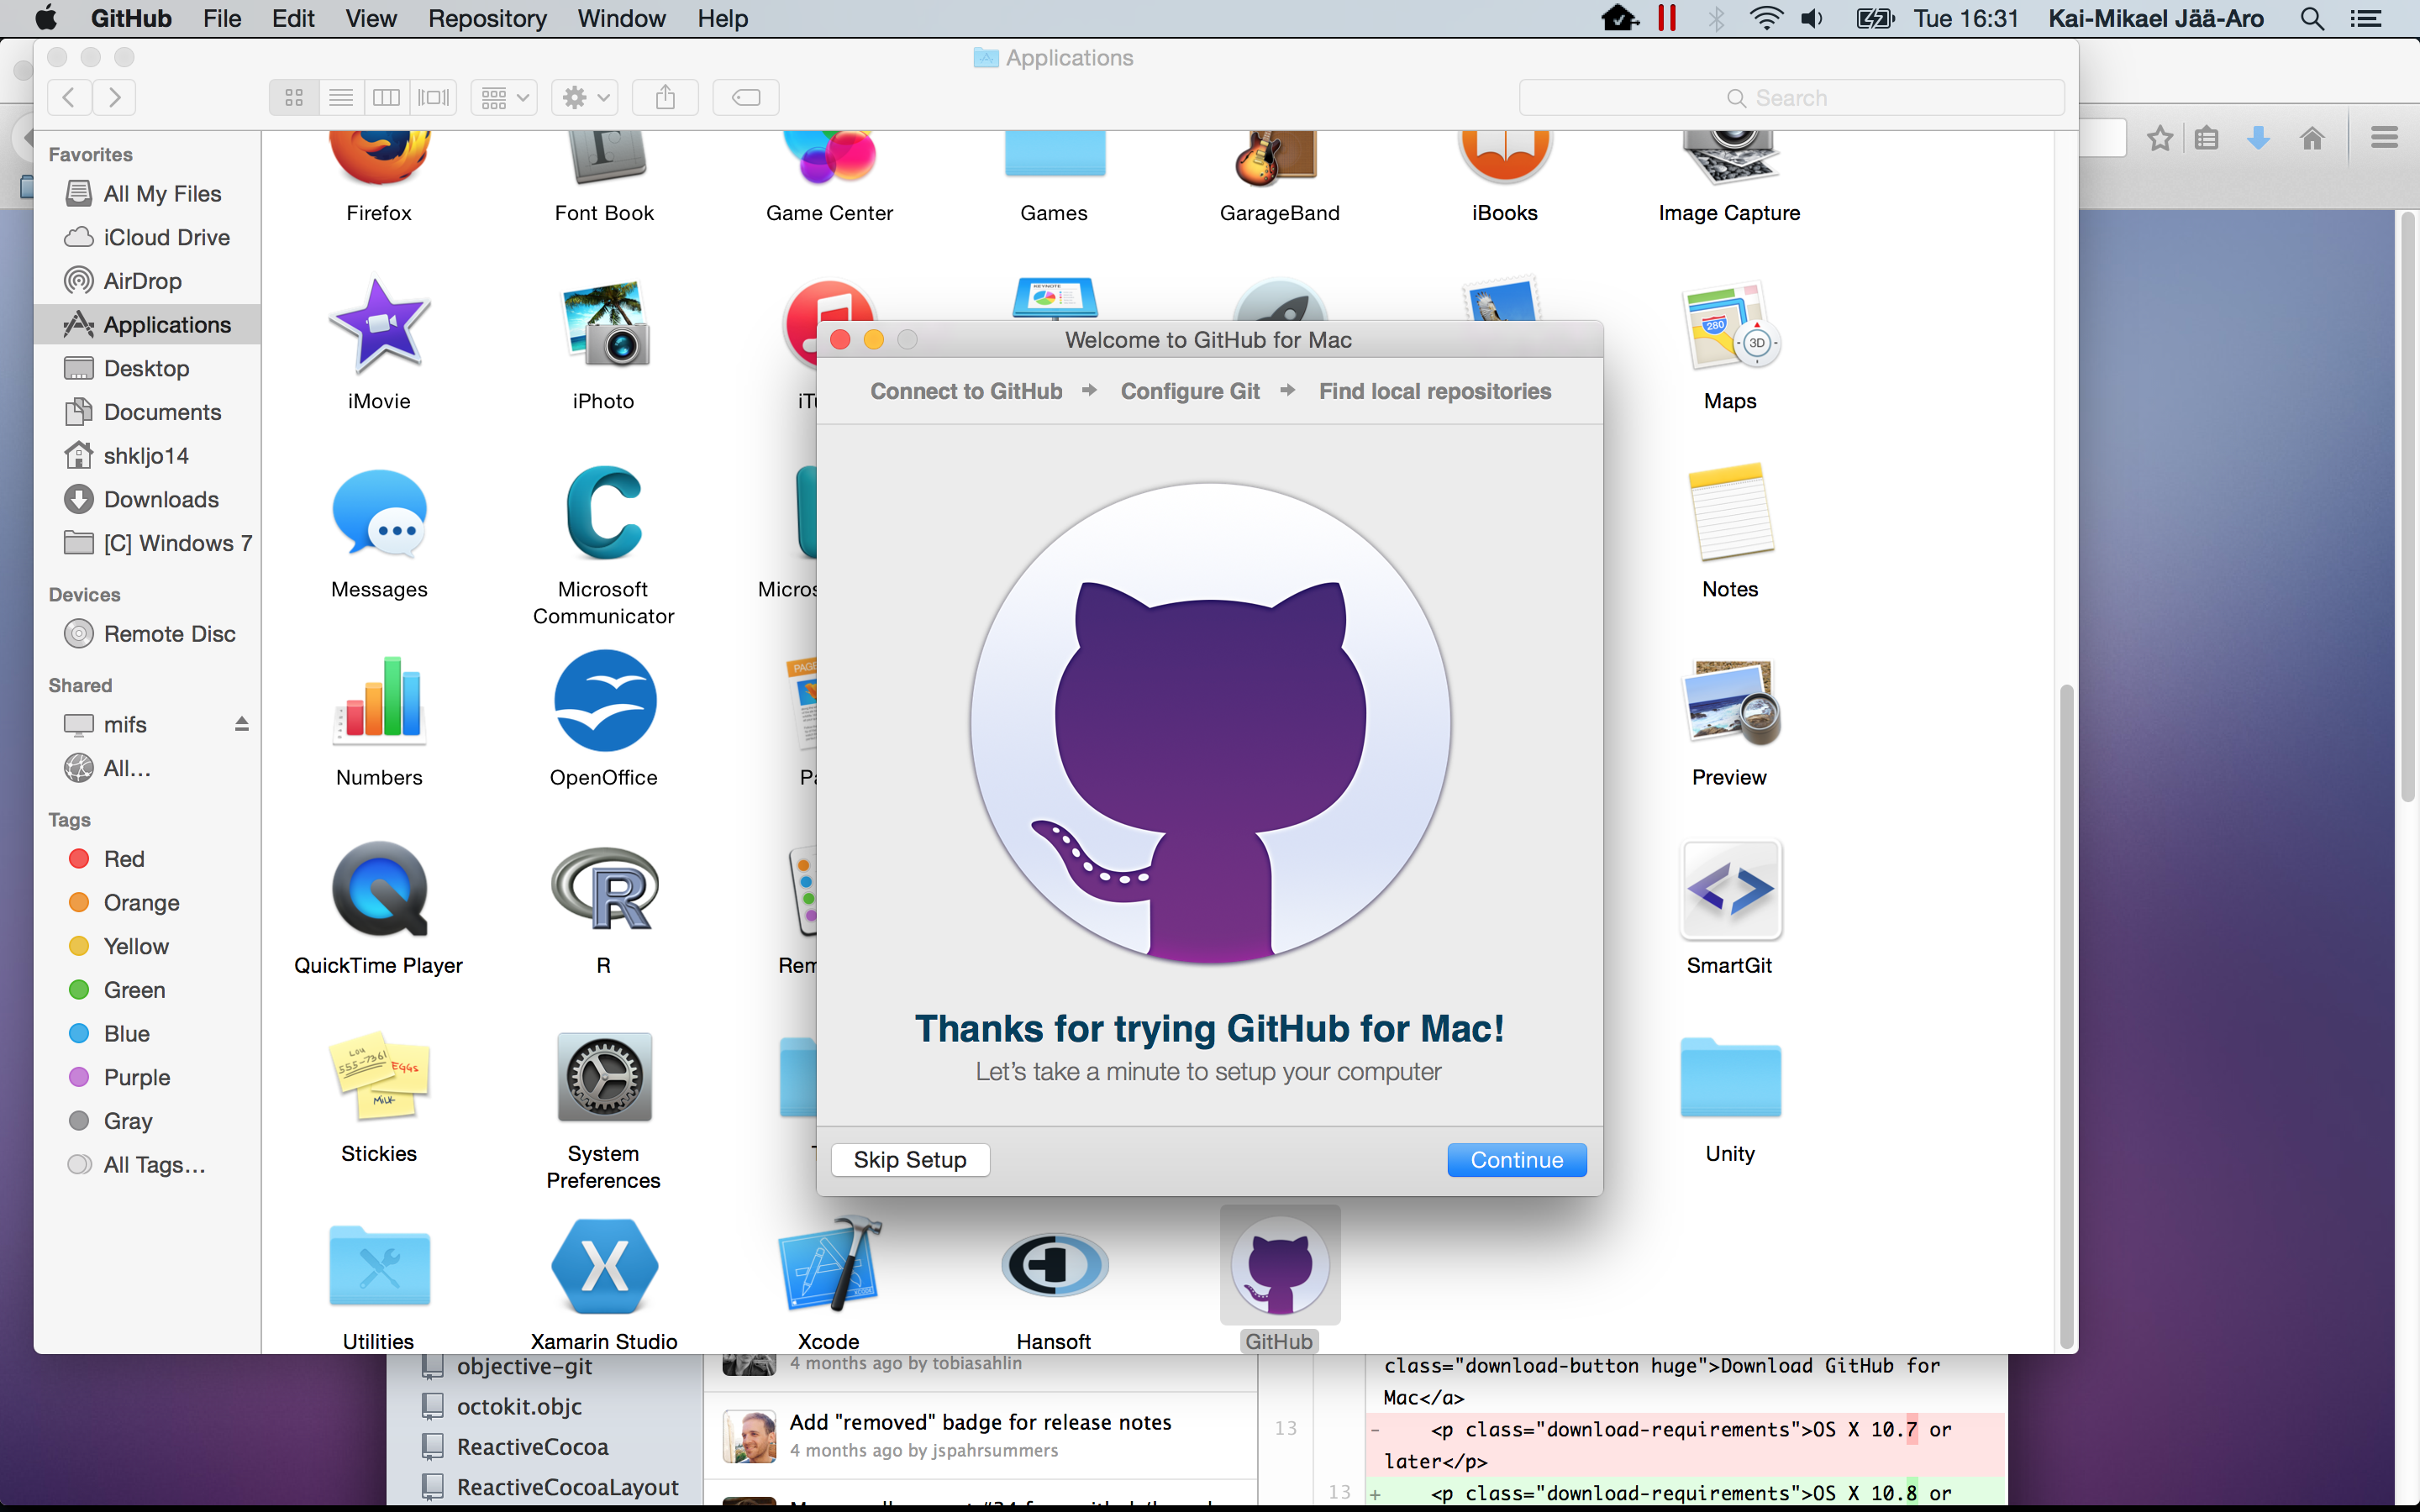
\includegraphics{GitHubWelcome}
\end{frame}

\begin{frame}
\frametitle{Logga in på arkivet}
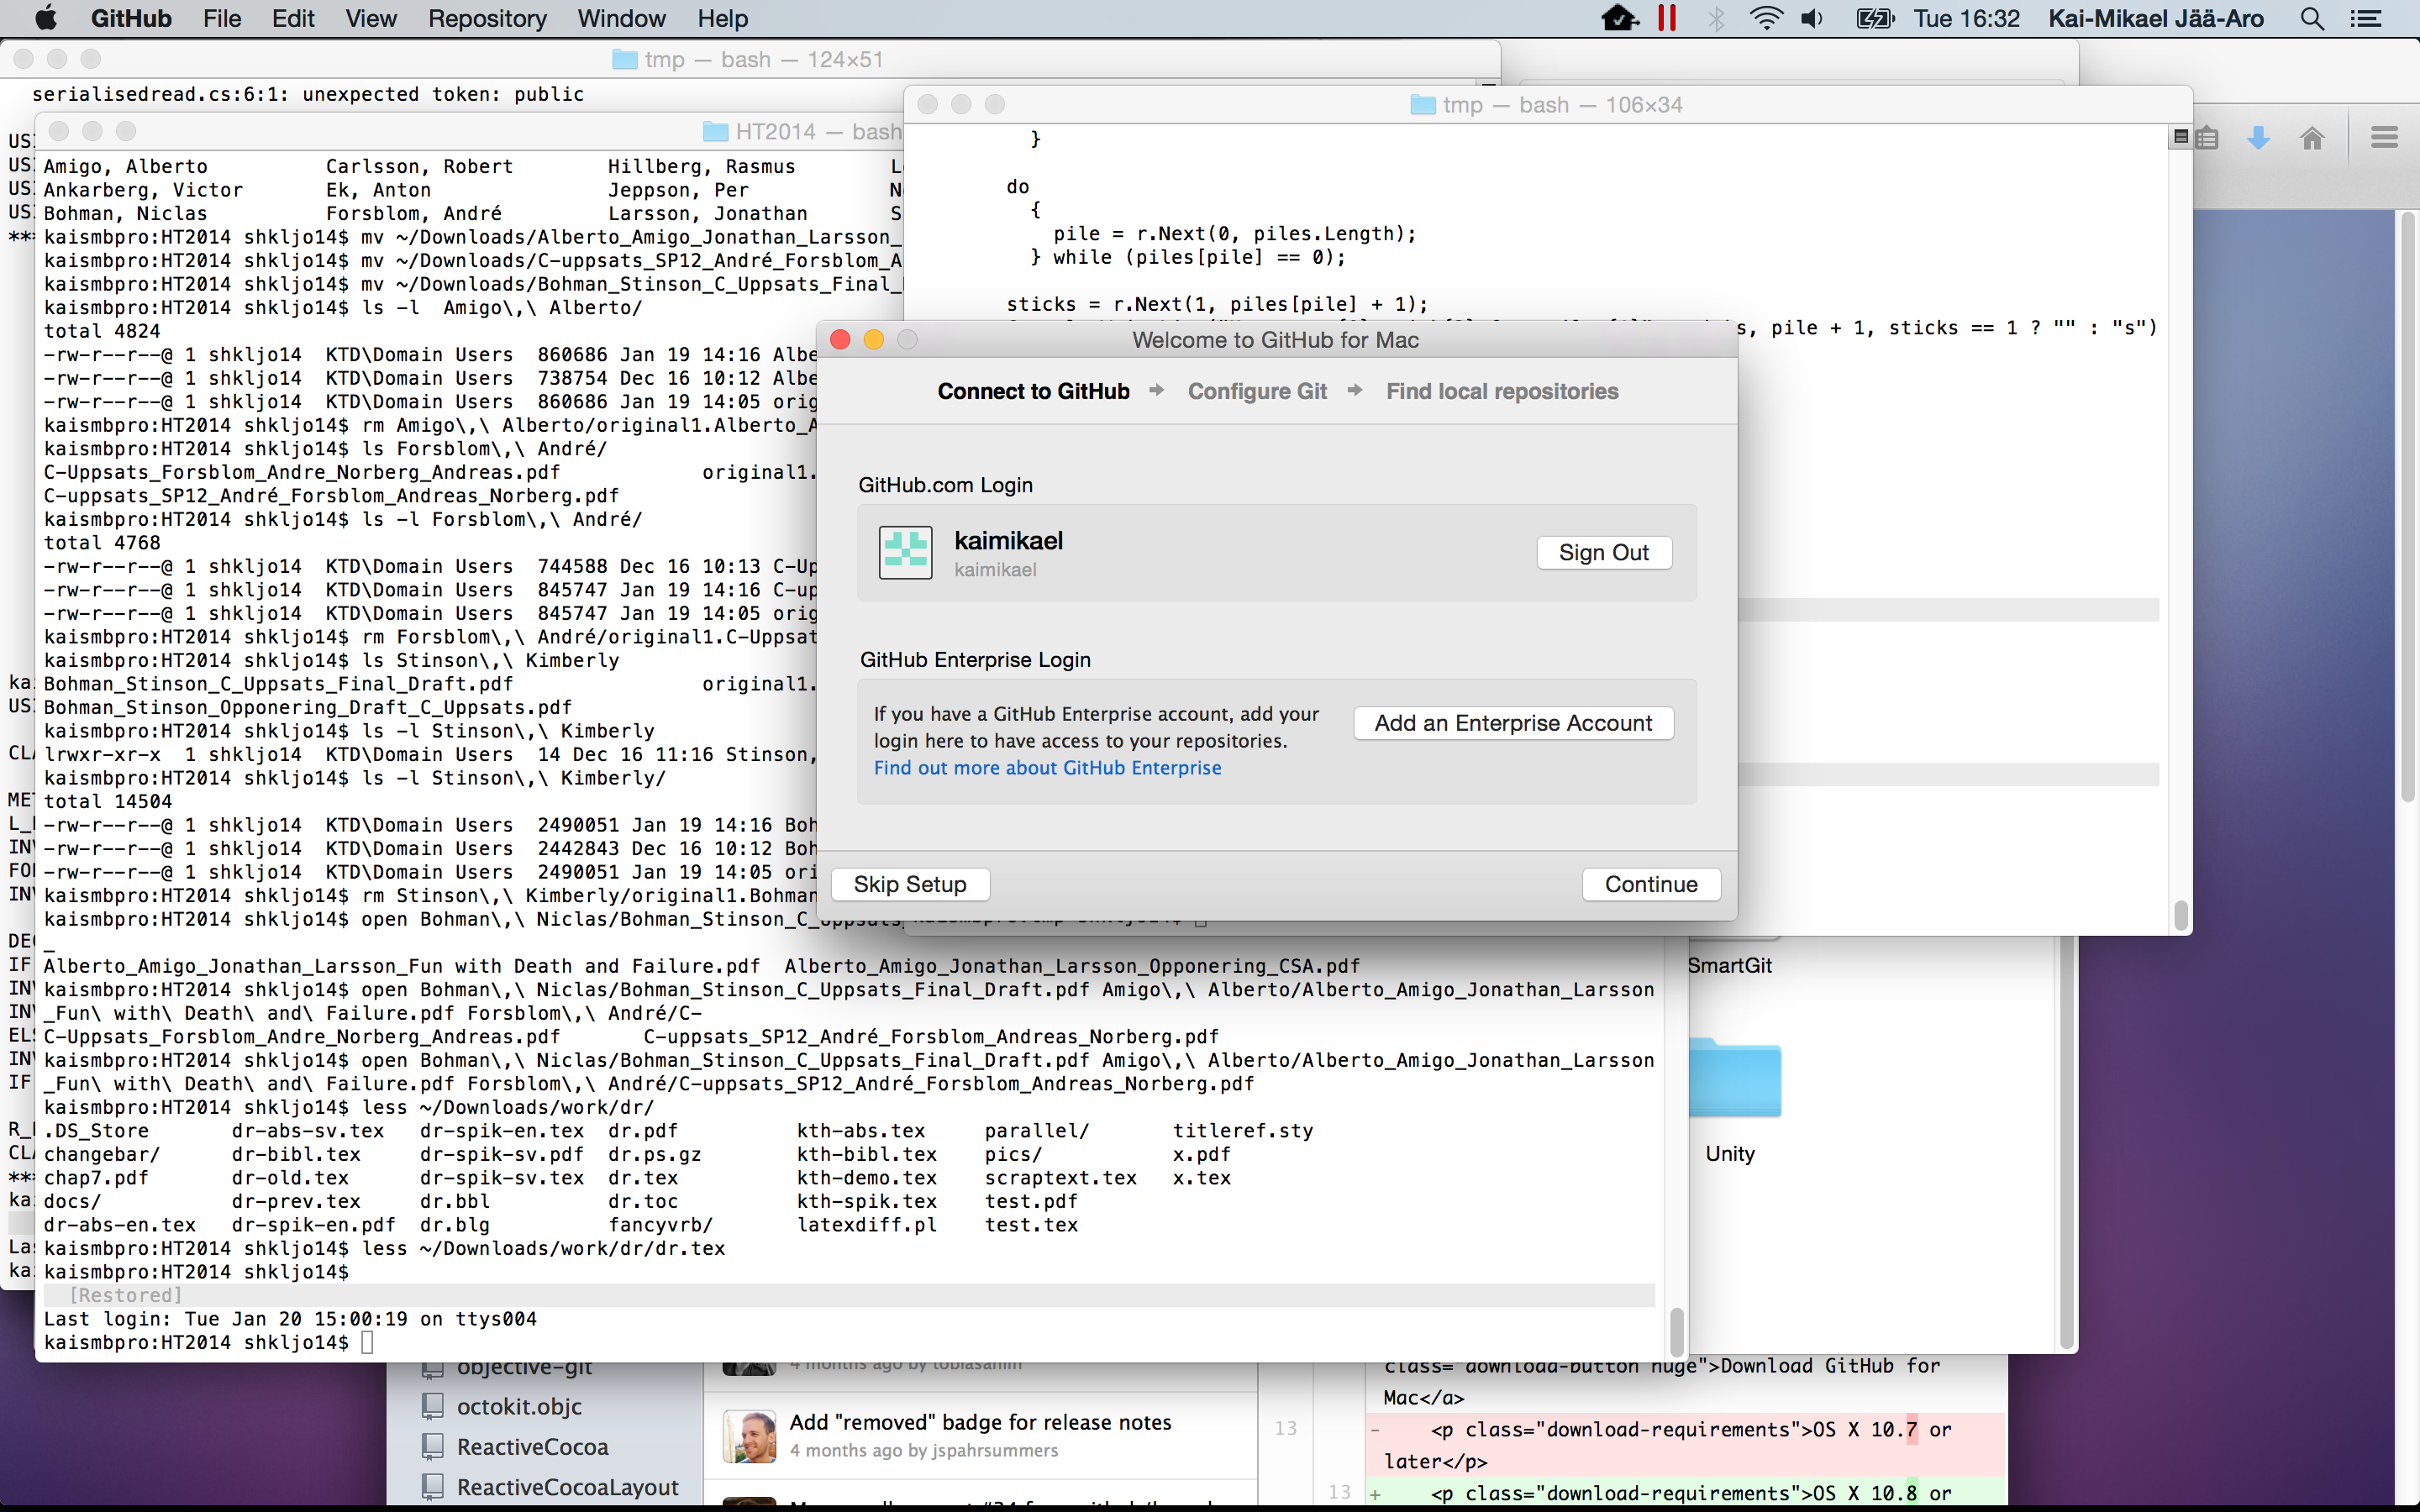
\includegraphics{GitHubLogin}
\end{frame}

\begin{frame}
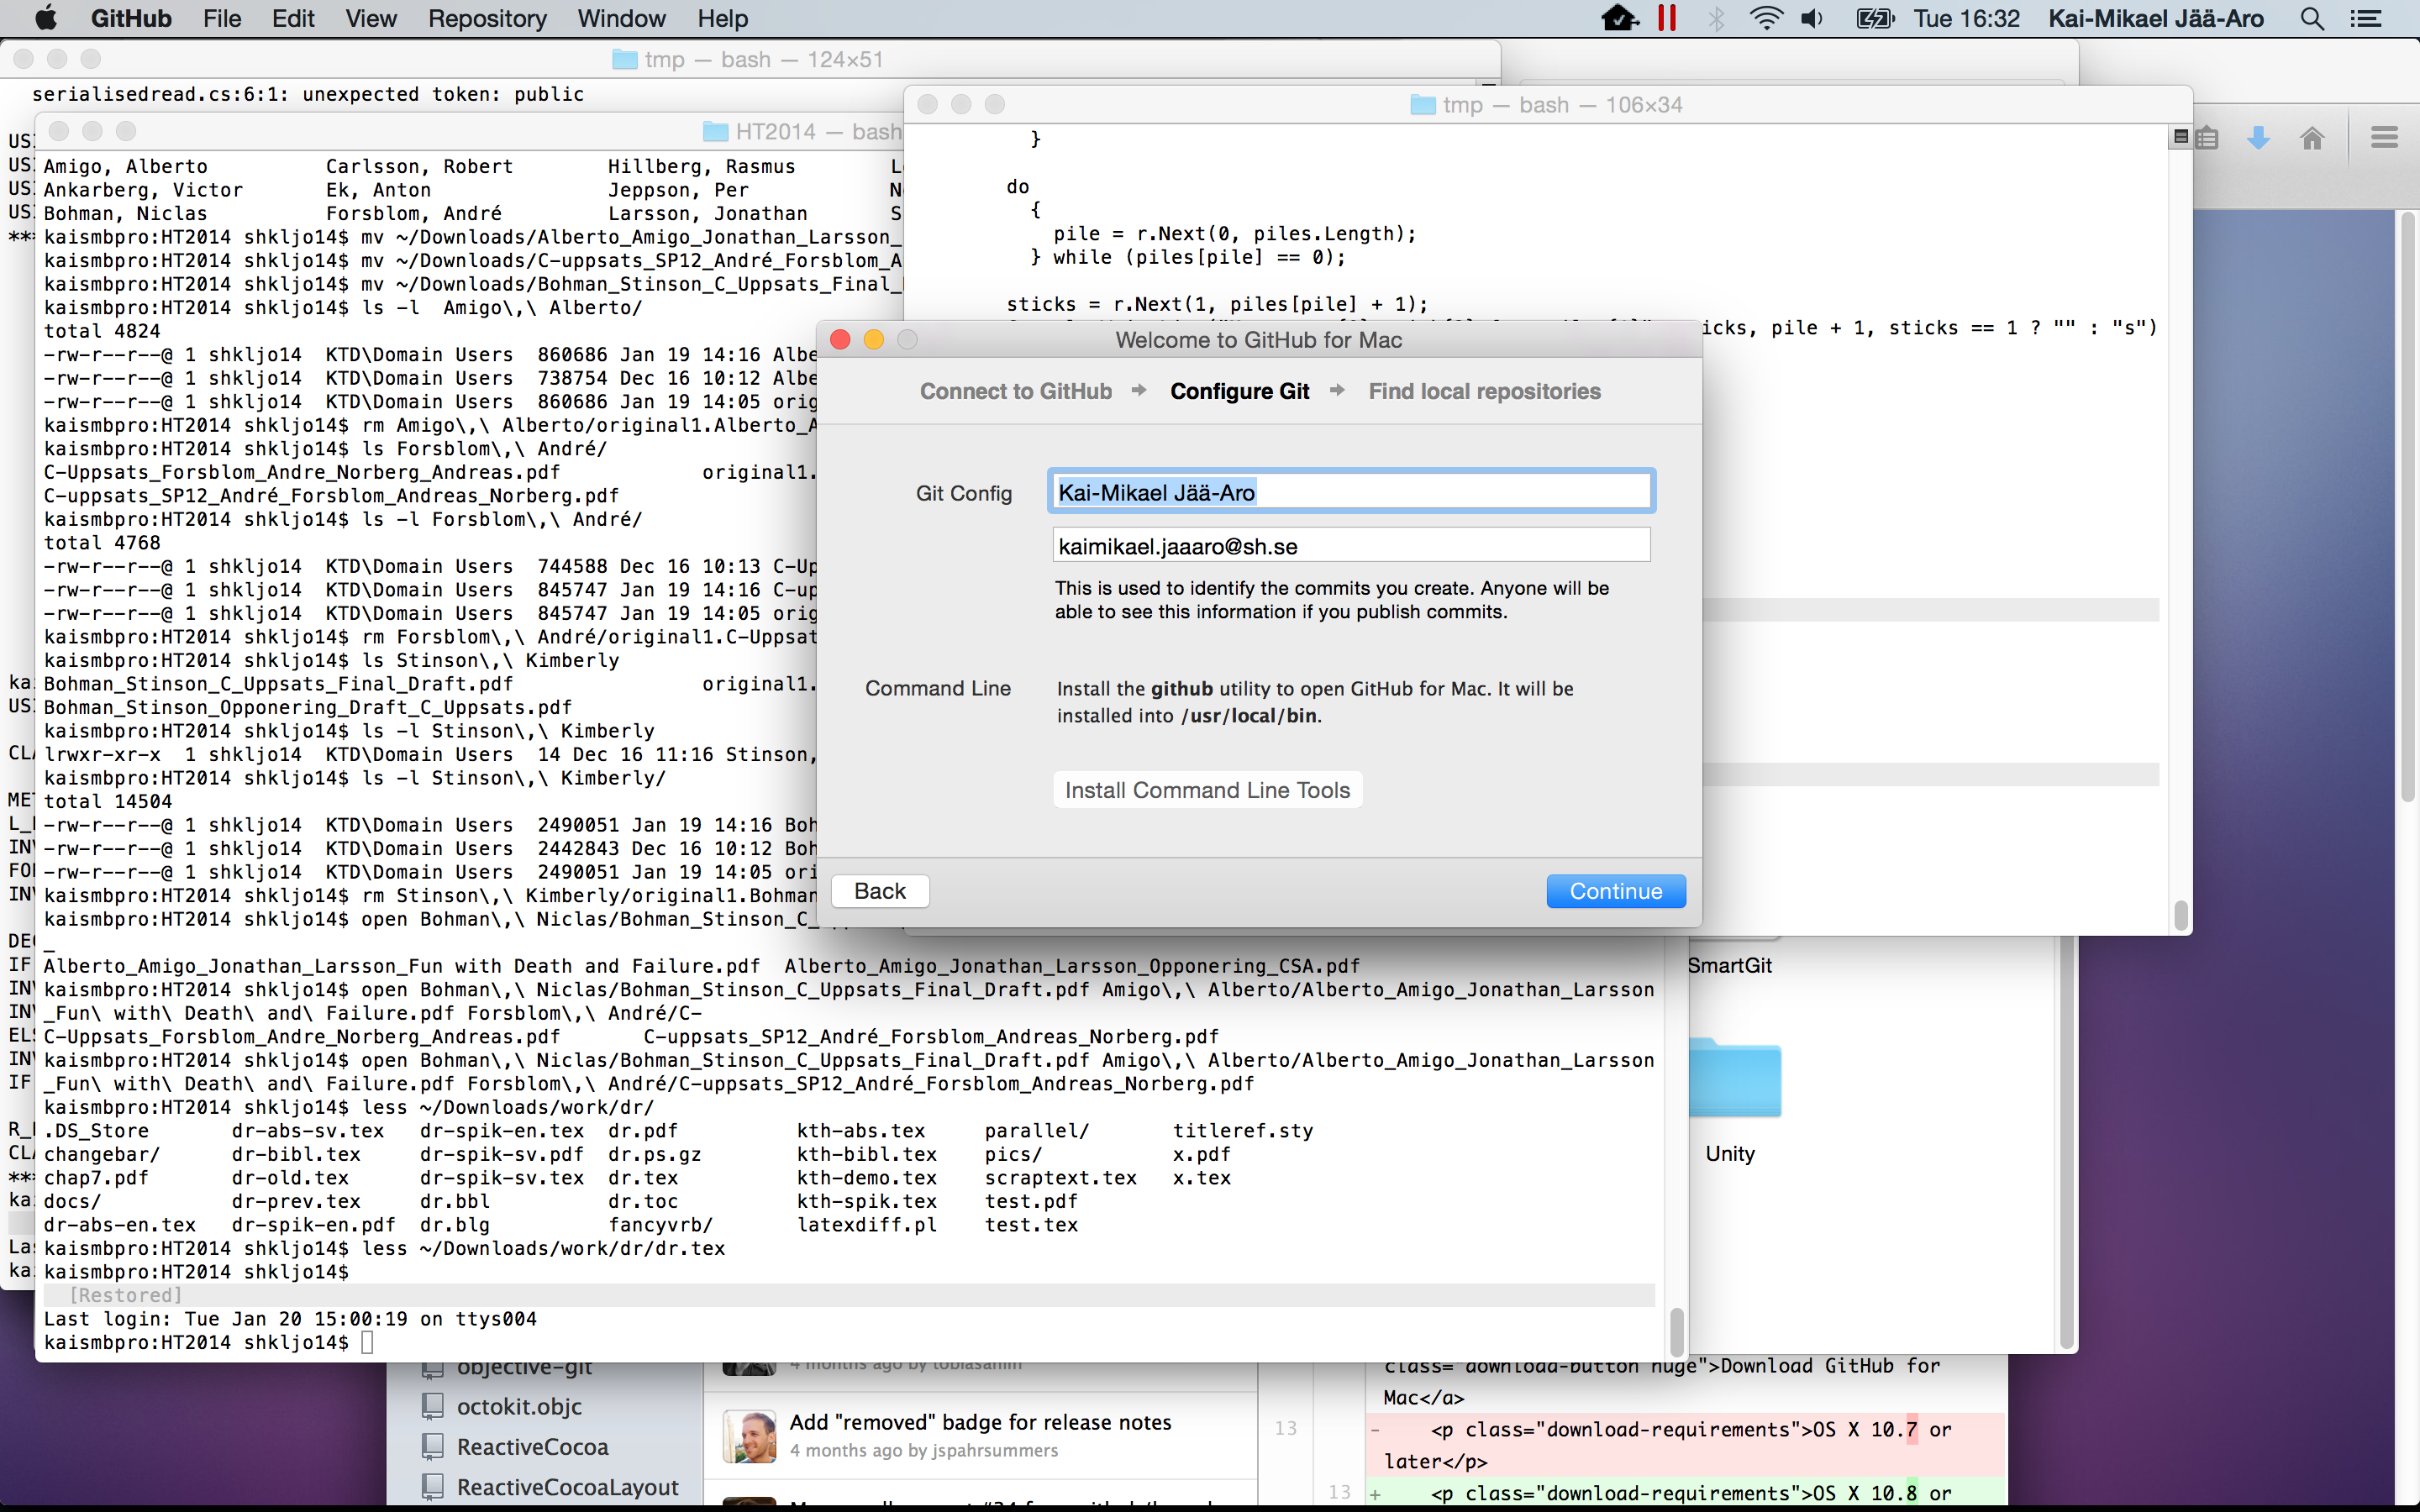
\includegraphics{GitHubConfig}
\end{frame}

\begin{frame}
\frametitle{Hitta lokala arkiv}
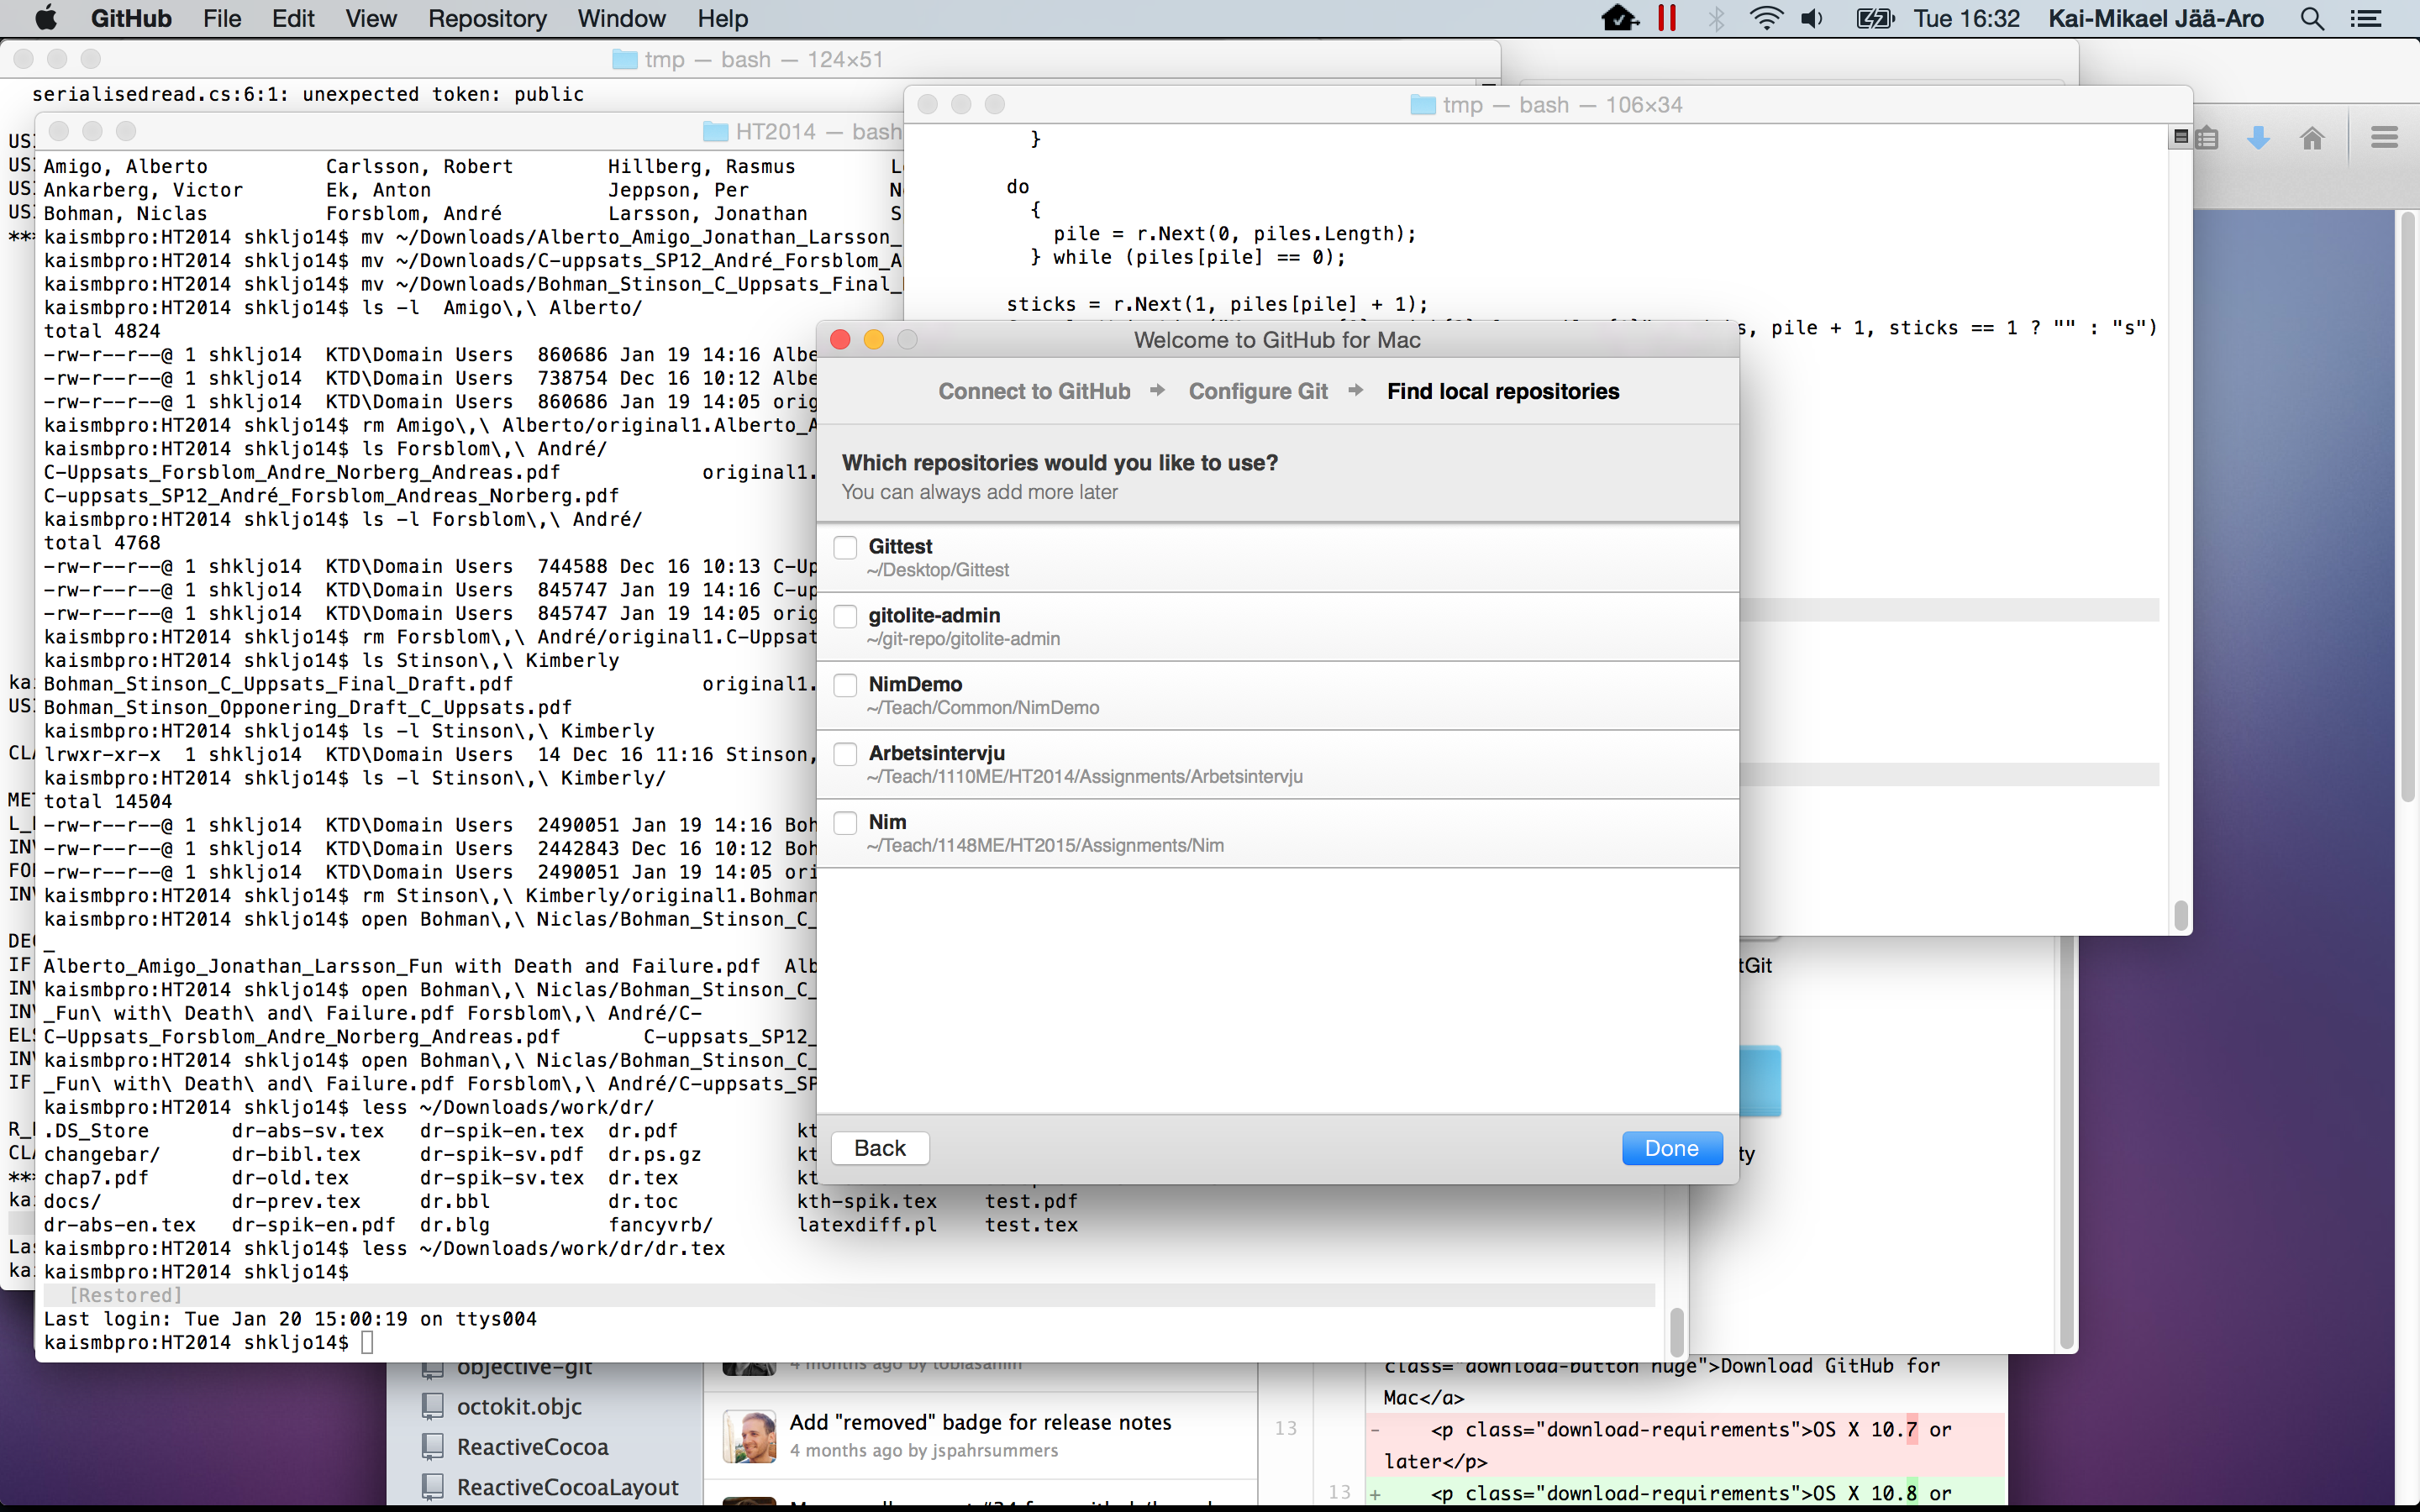
\includegraphics{GitHubFindLocalRepositories}
\end{frame}


\begin{frame}
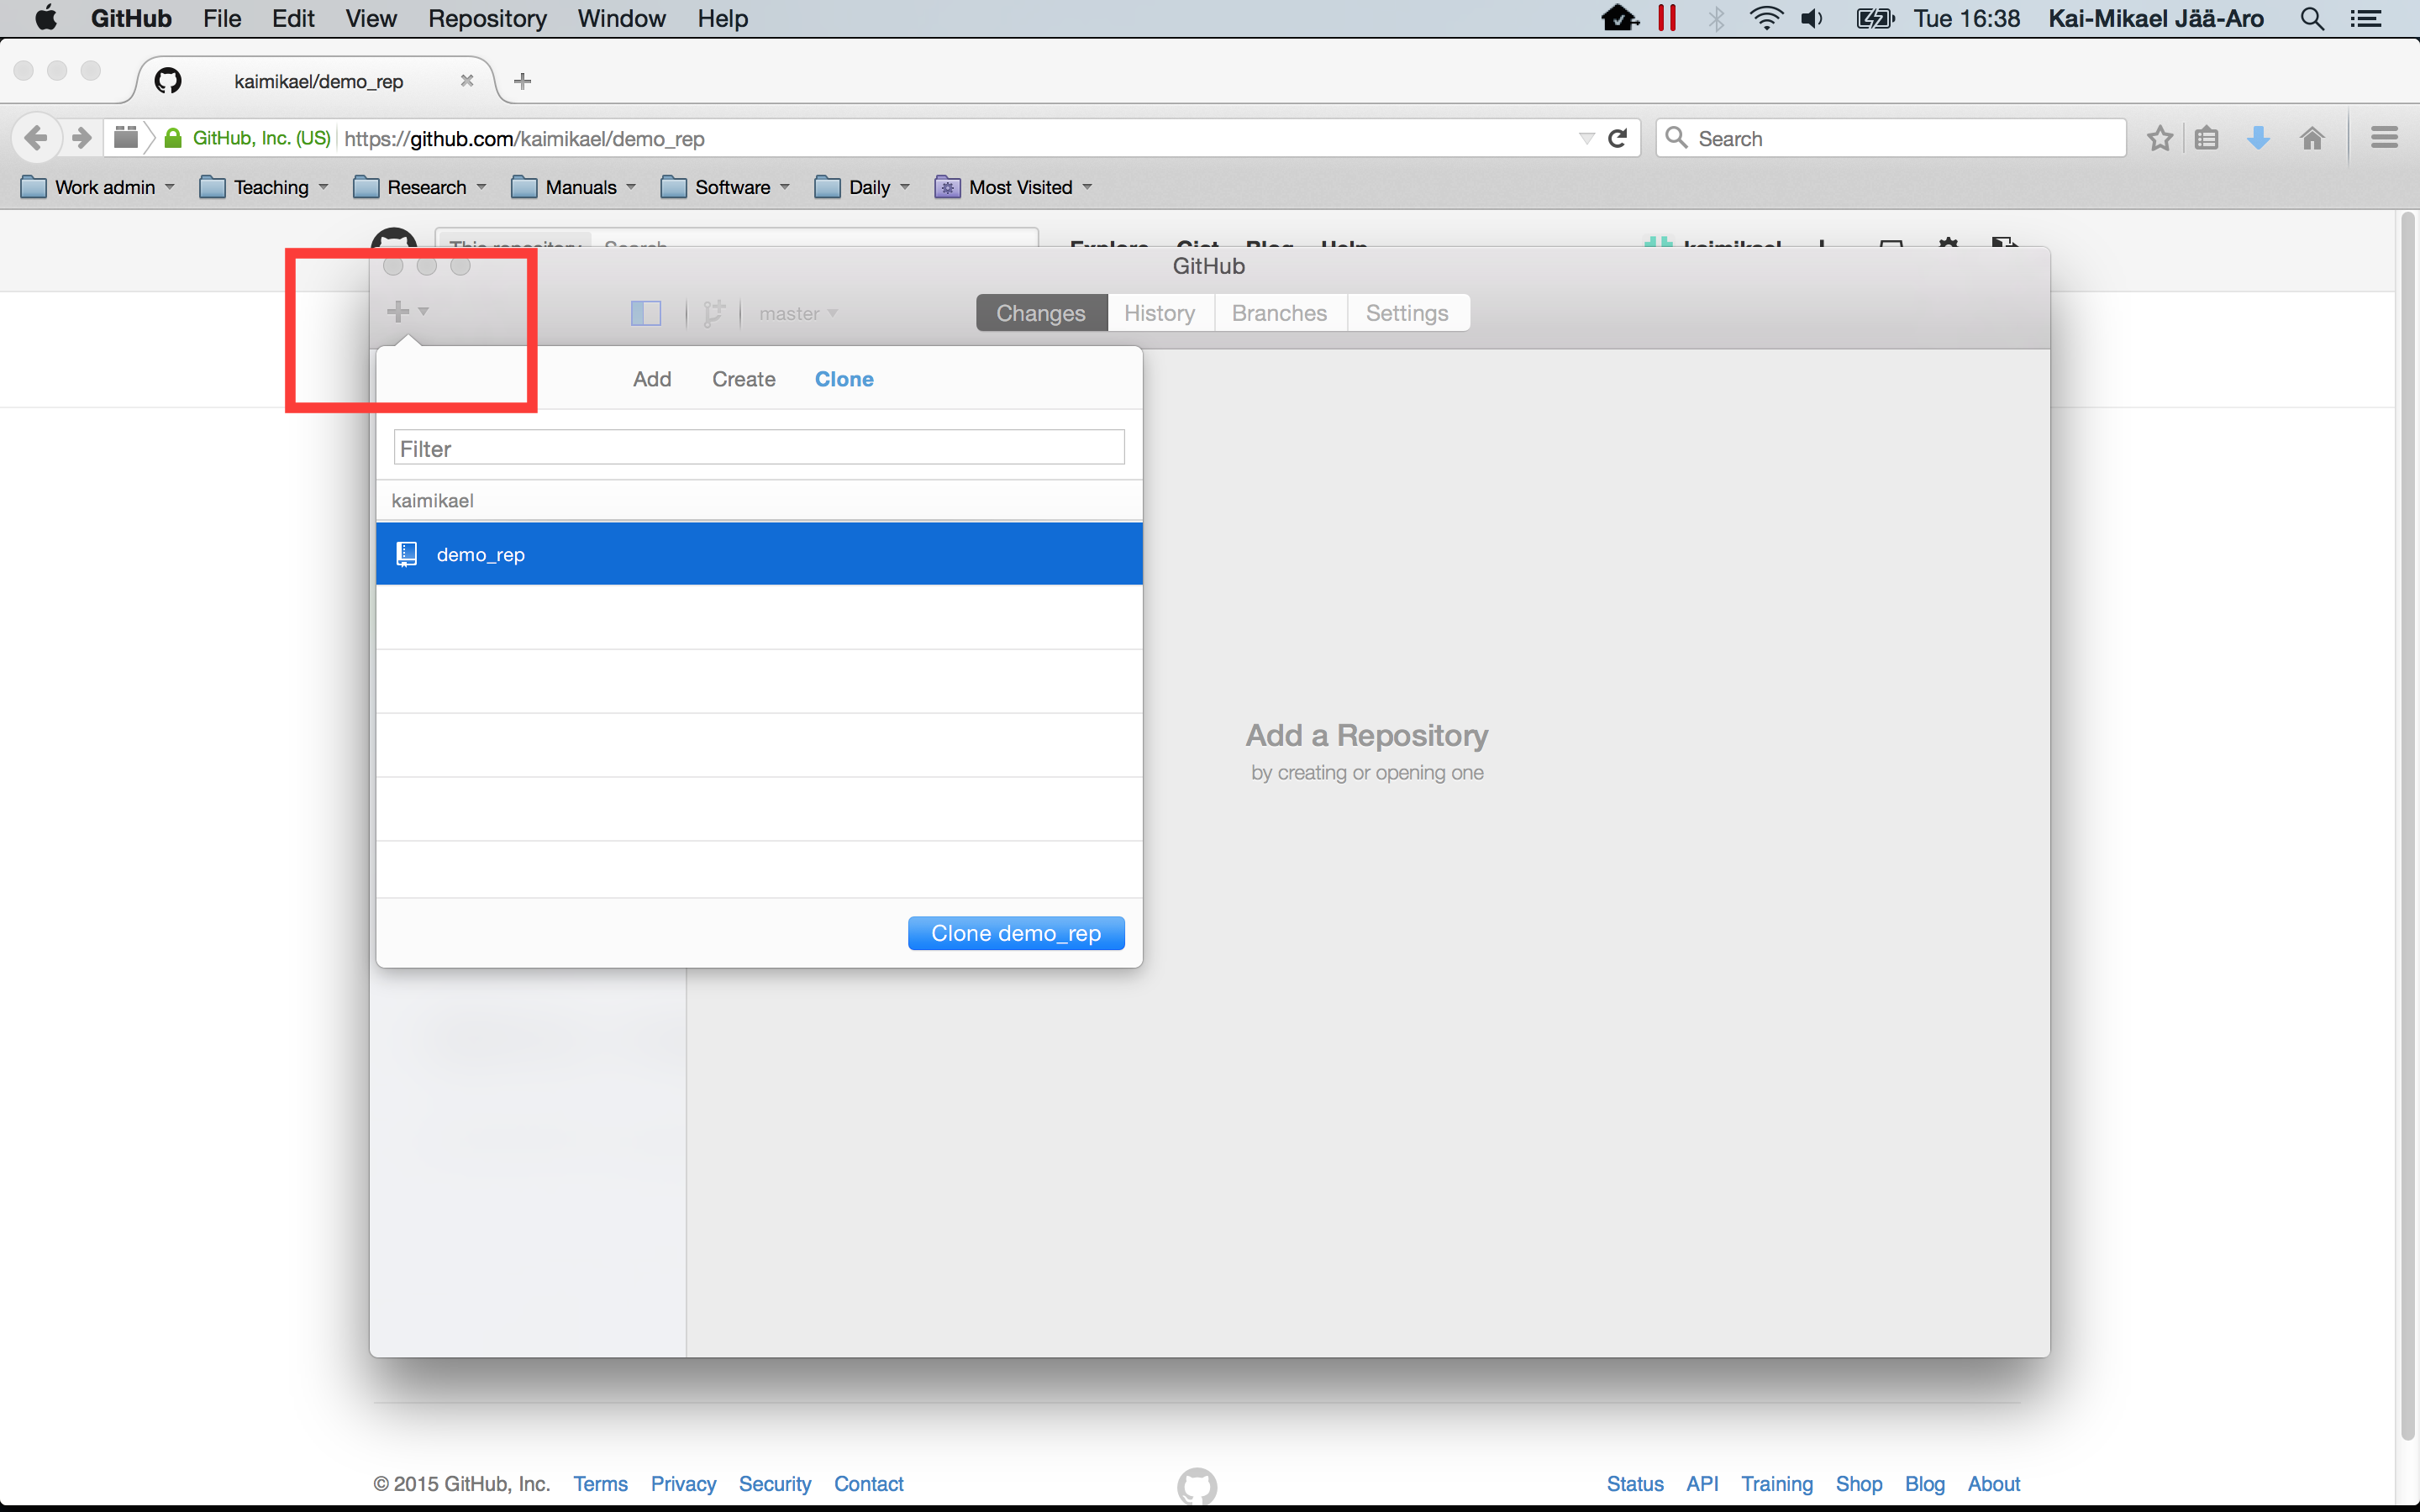
\includegraphics{GitHubCloneRepository}
\end{frame}

\begin{frame}
\frametitle{Lägg till filer i arkivet}
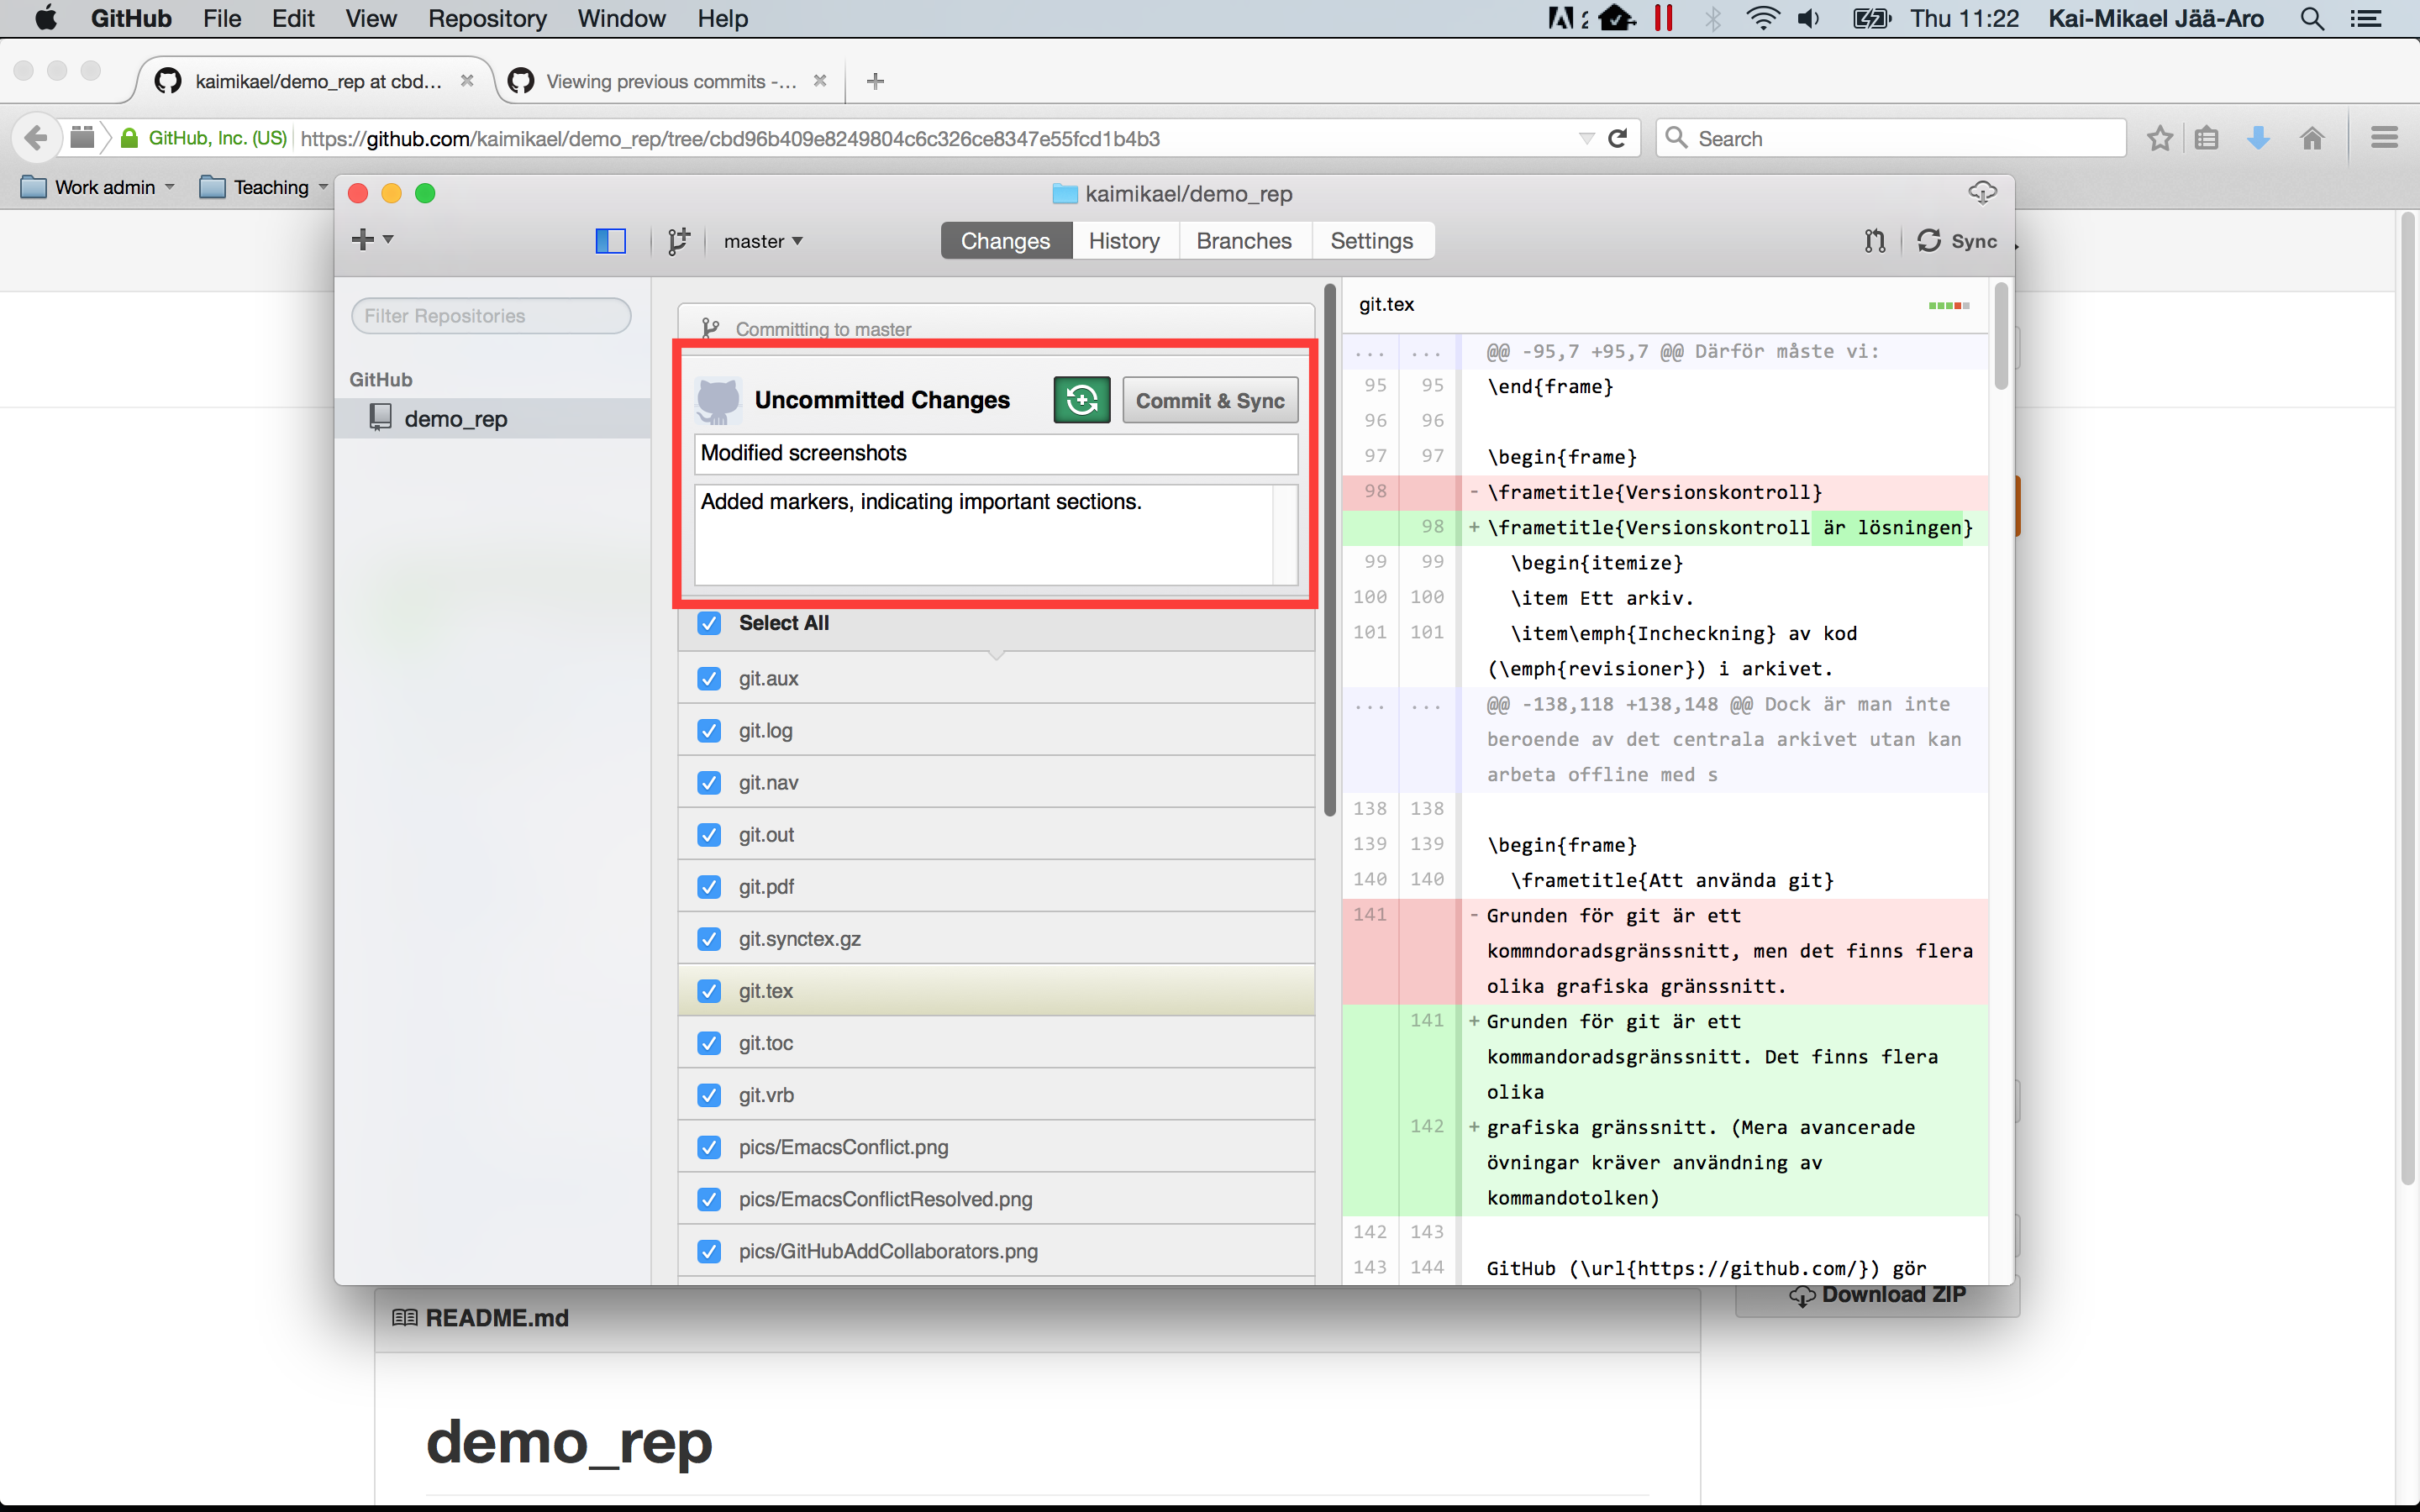
\includegraphics{GitHubAddFiles}
\end{frame}

\begin{frame}
\frametitle{Checka in uppdaterade filer}
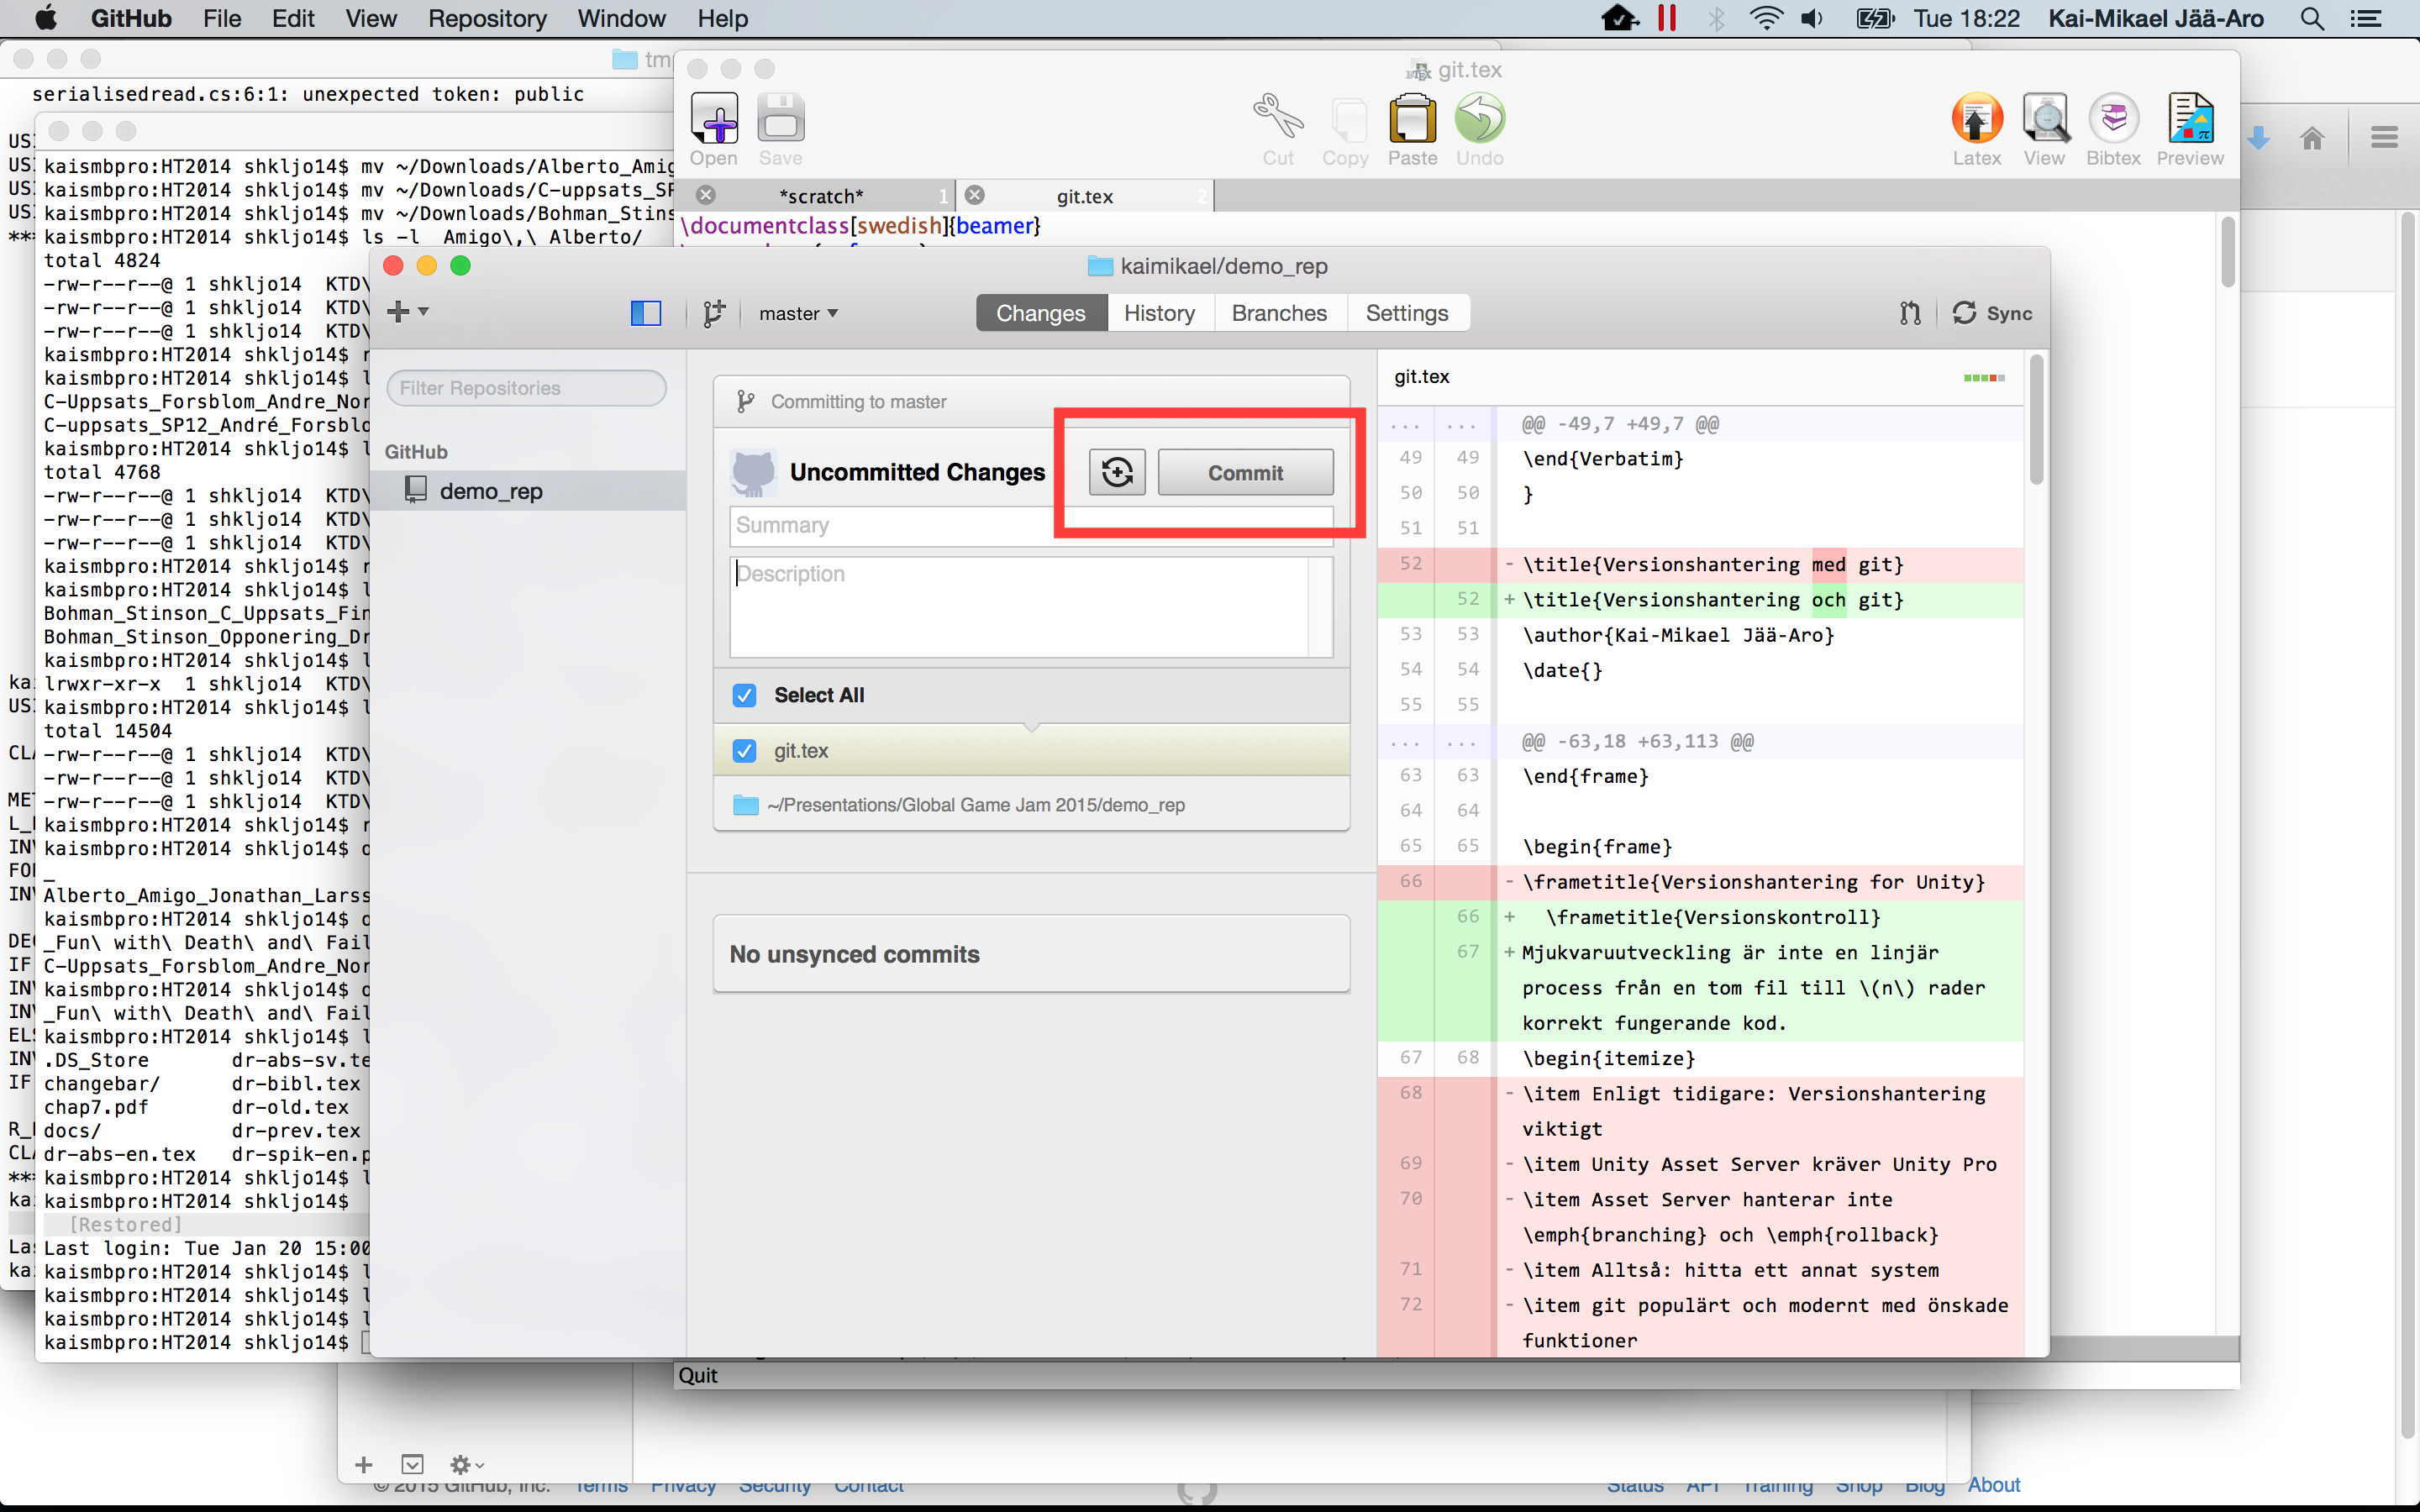
\includegraphics{GitHubCommitChanges}
\end{frame}

\begin{frame}
Om flera utvecklare ändrar på samma ställe i en fil uppstår en
\emph{konflikt}.  Detta markeras i klienten, men måste lösas manuellt.

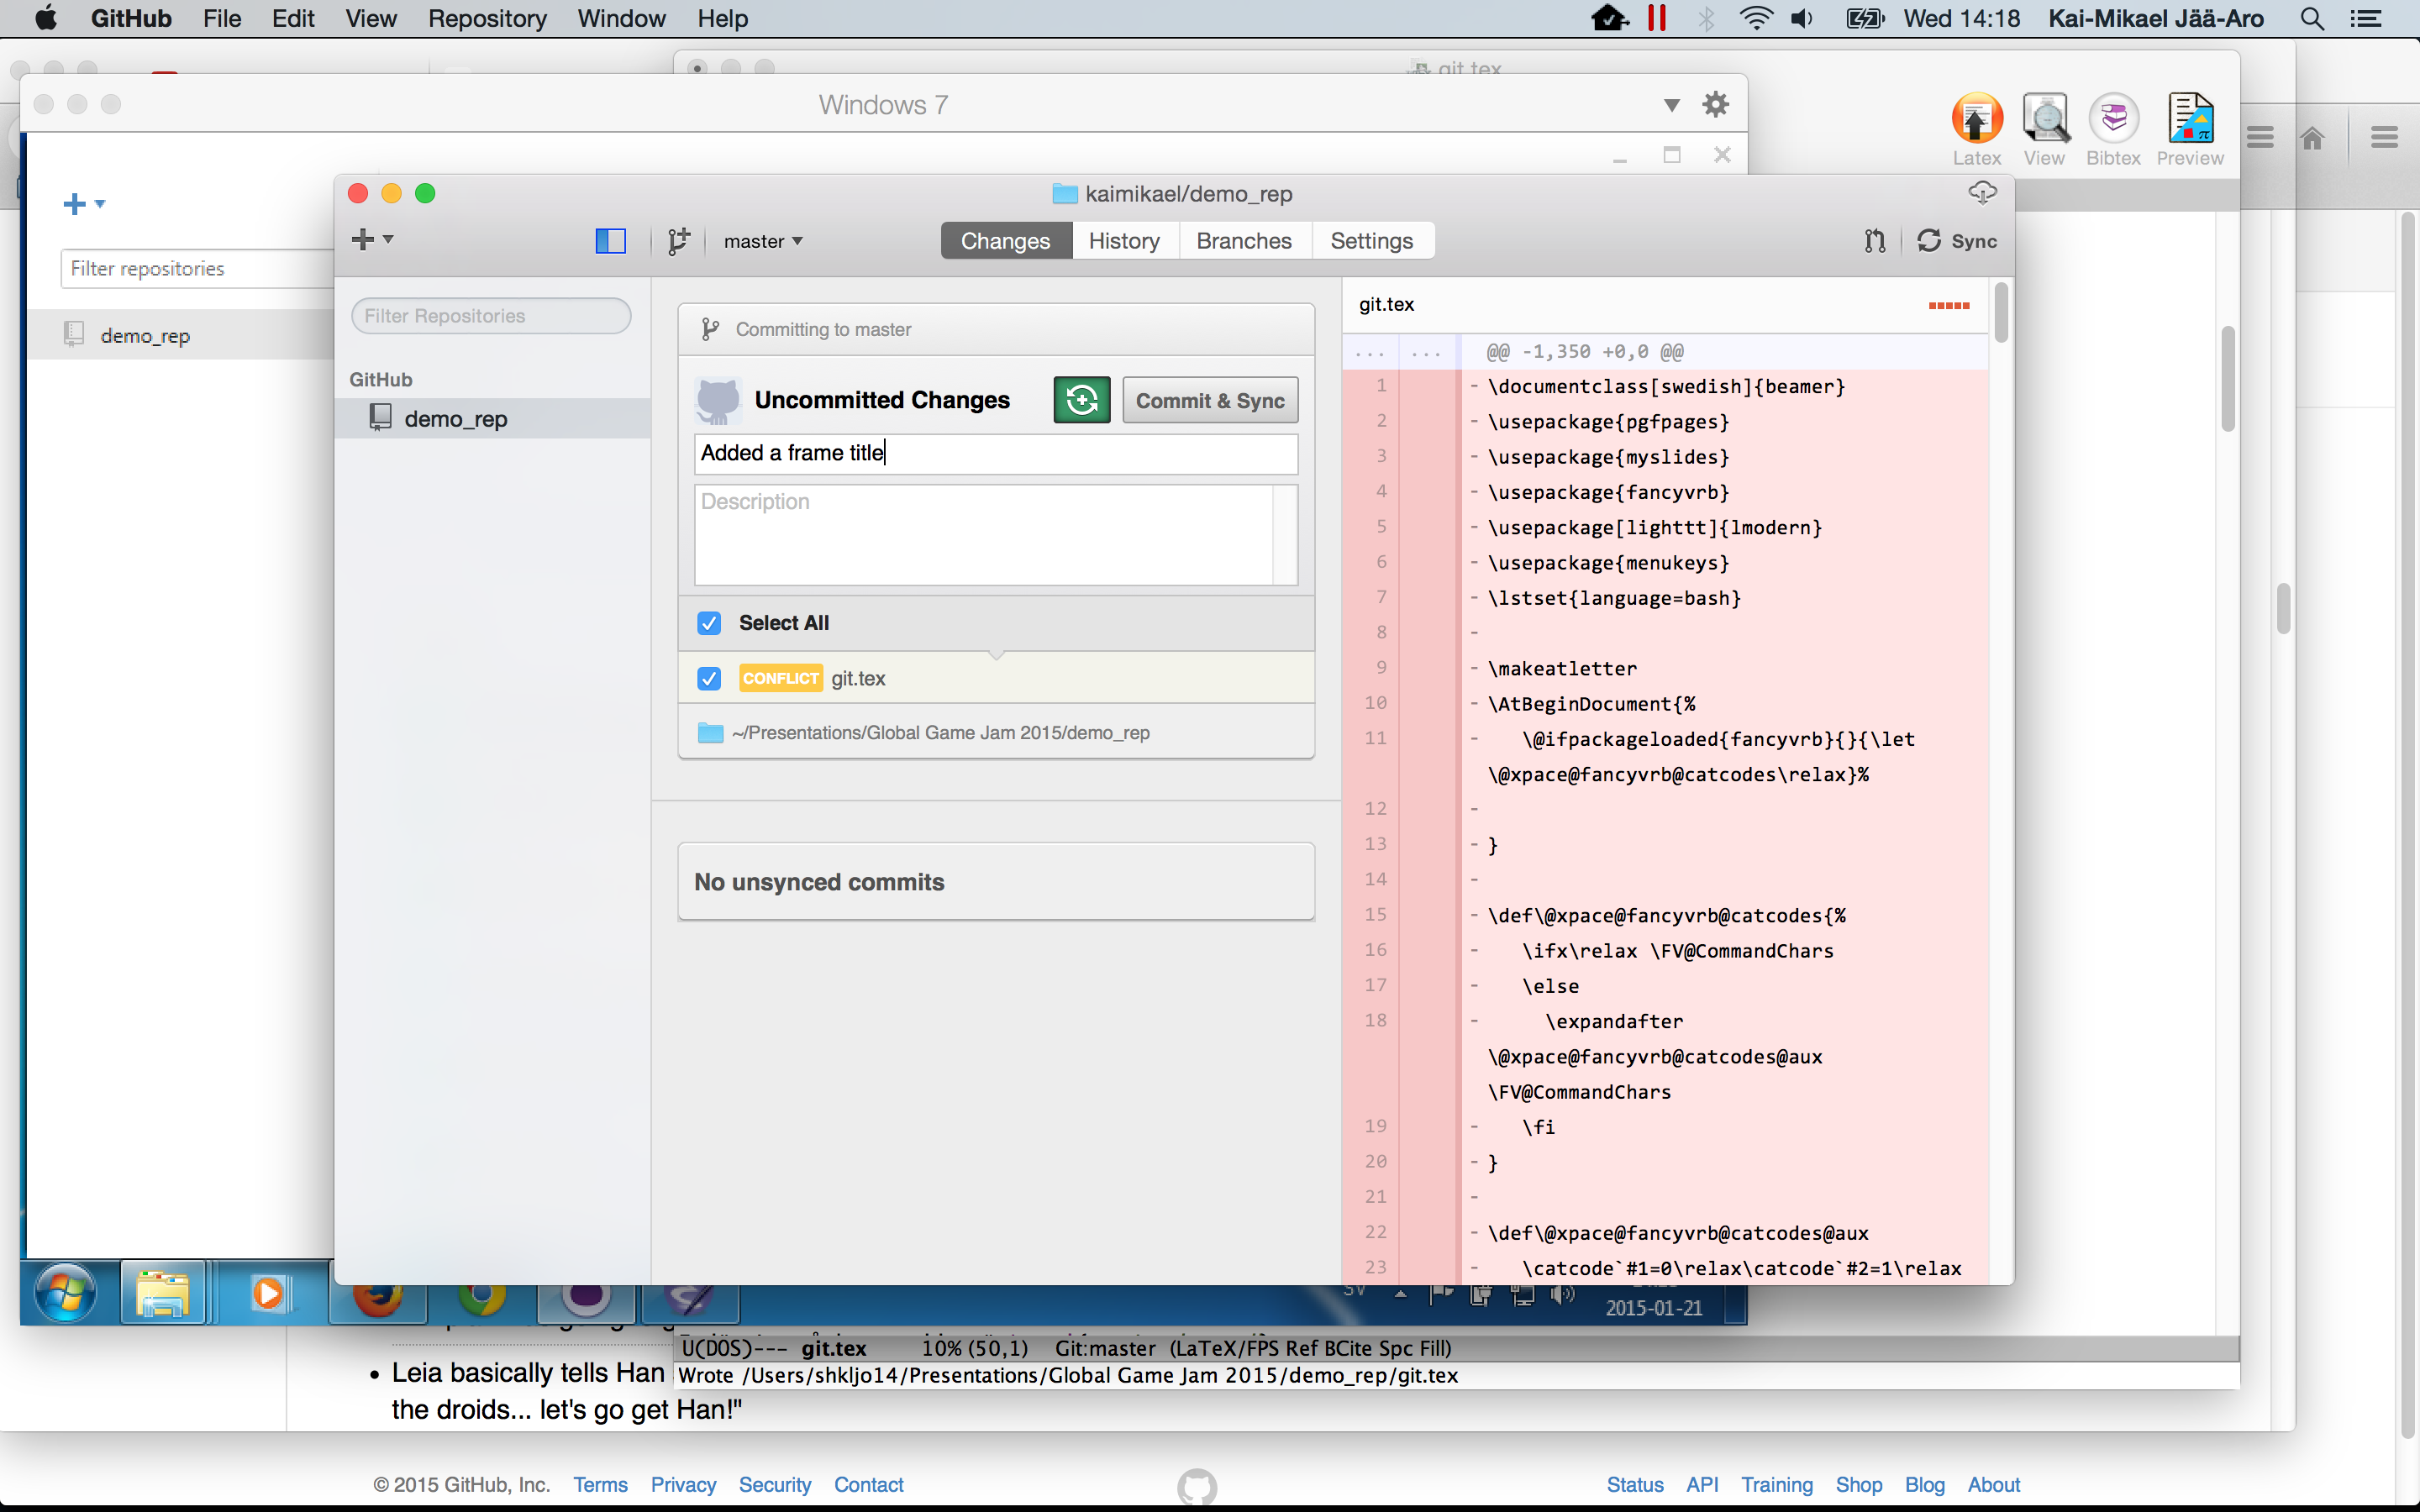
\includegraphics{GitHubConflict}
\end{frame}

\begin{frame}
Den synkroniserade filen har markörer vid konfliktpunkten.

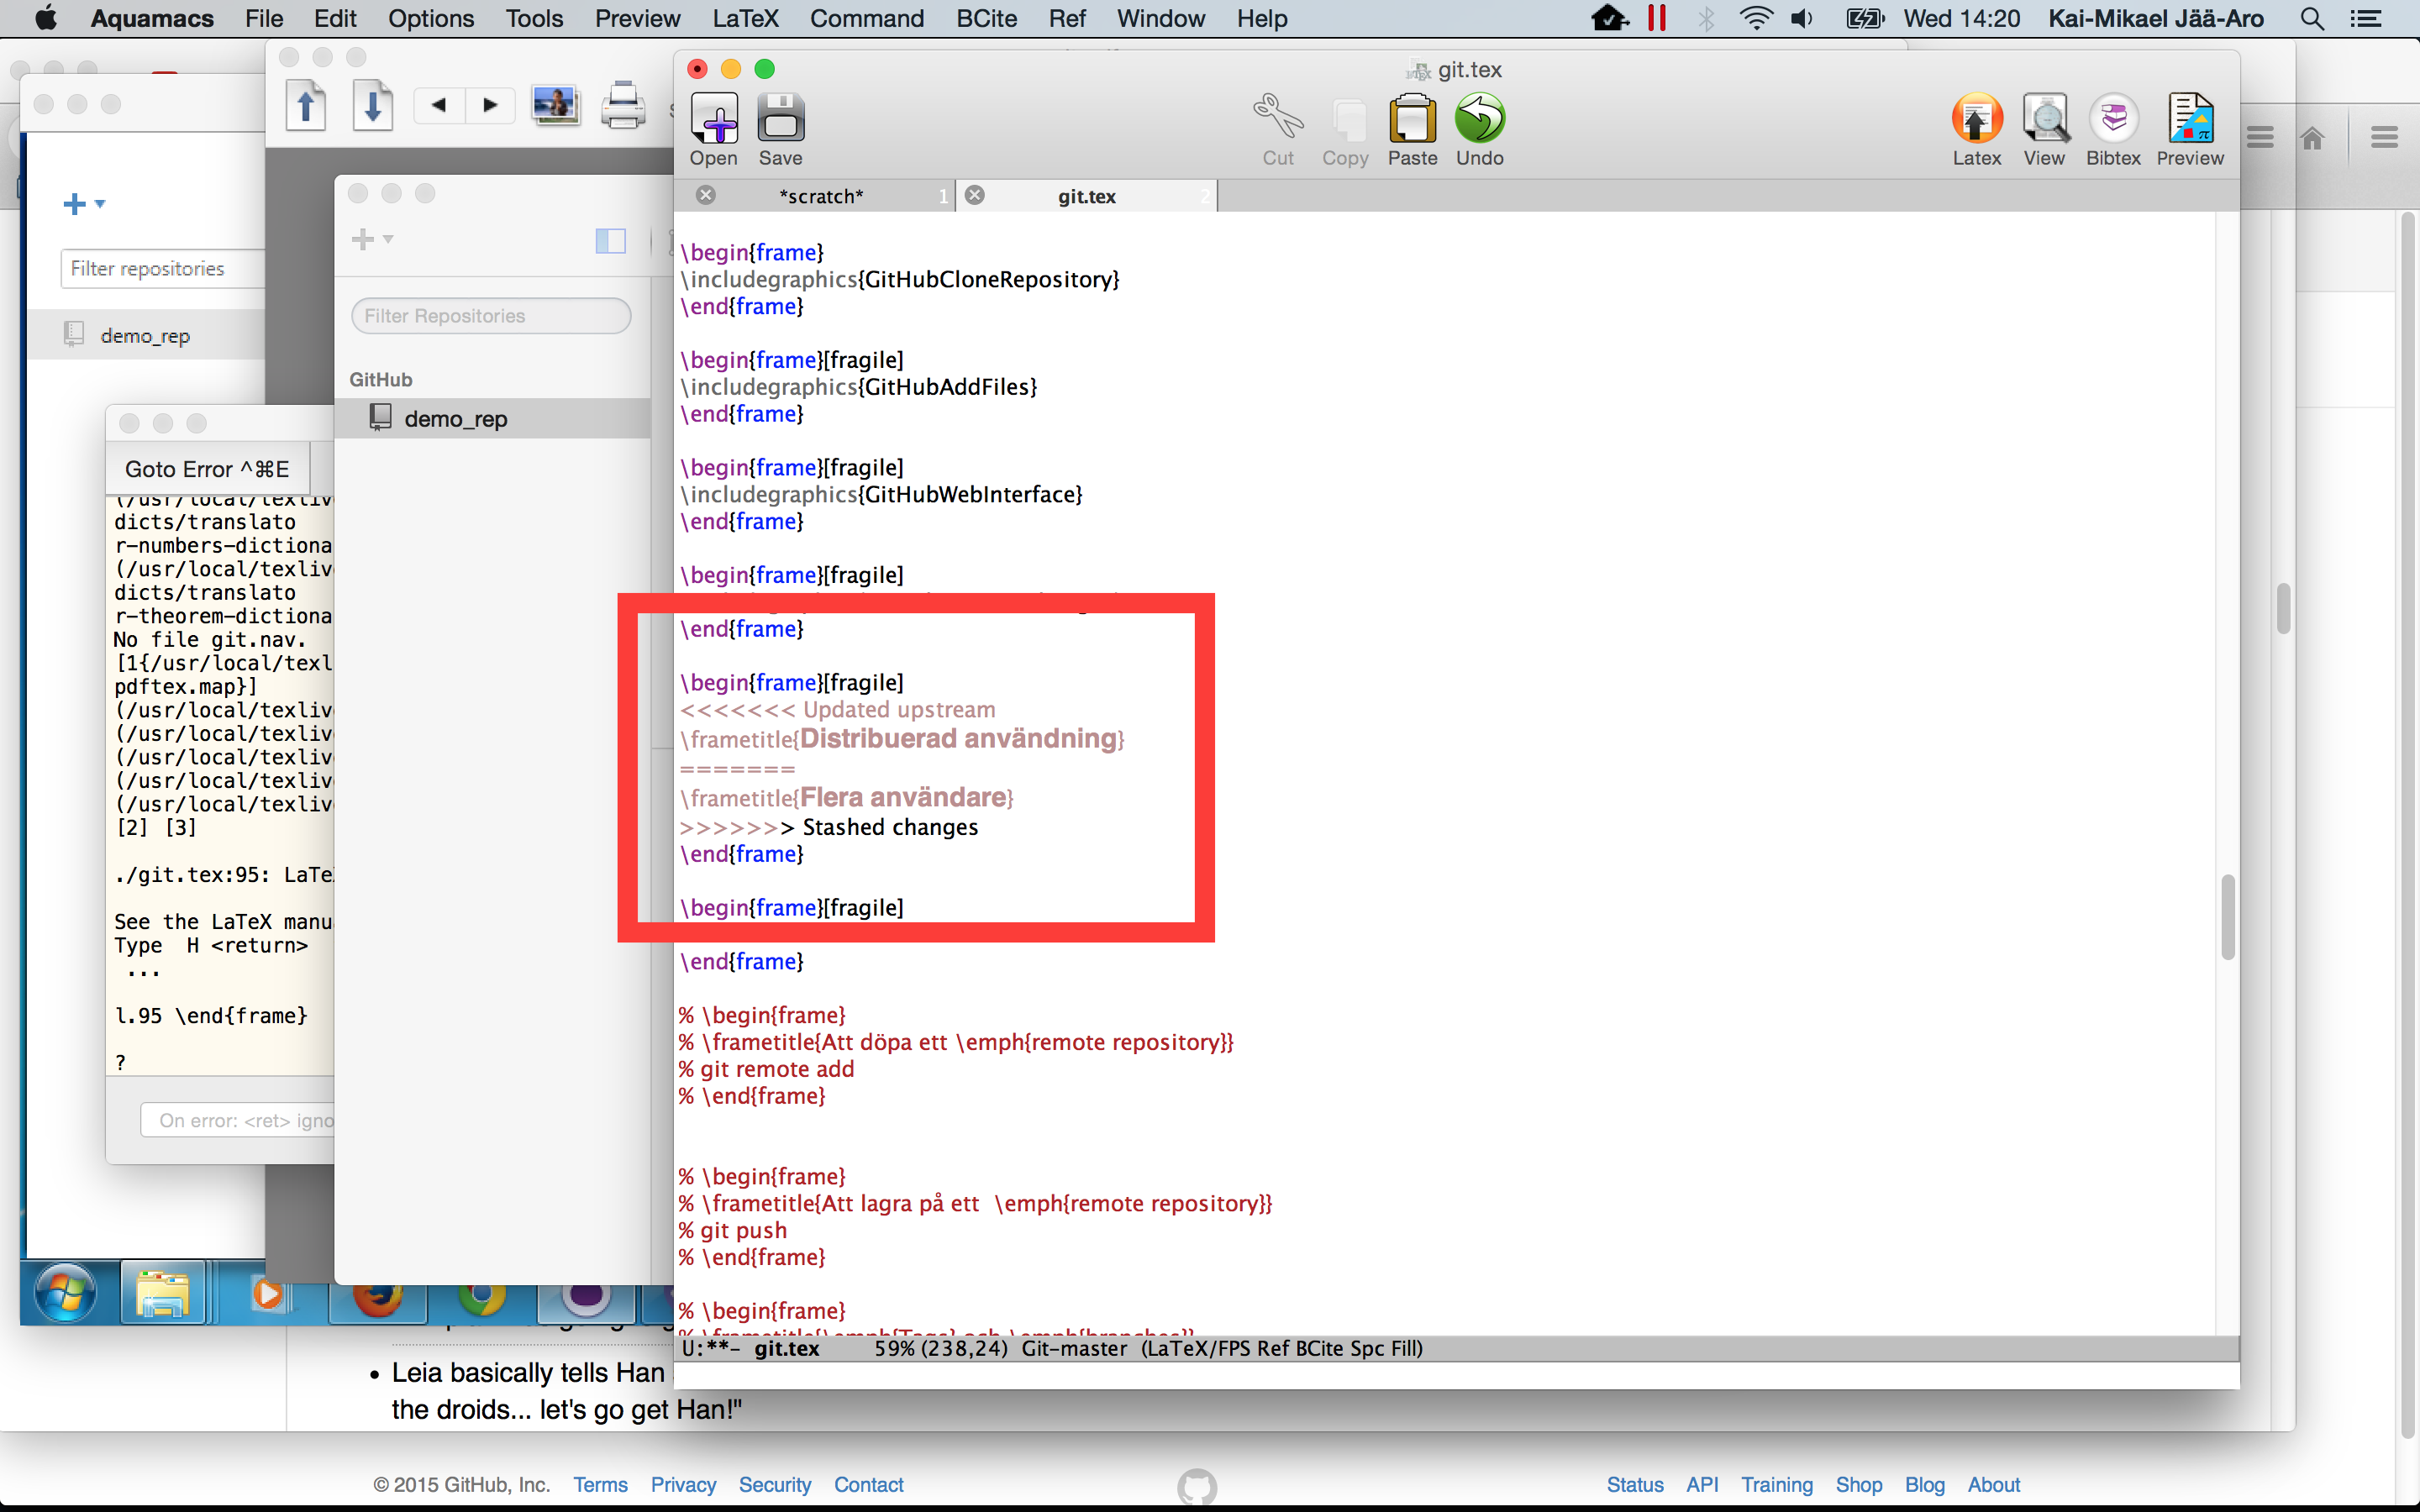
\includegraphics{EmacsConflict}
\end{frame}


\begin{frame}
Dessa ska hanteras manuellt och filen kan sedan checkas in igen.

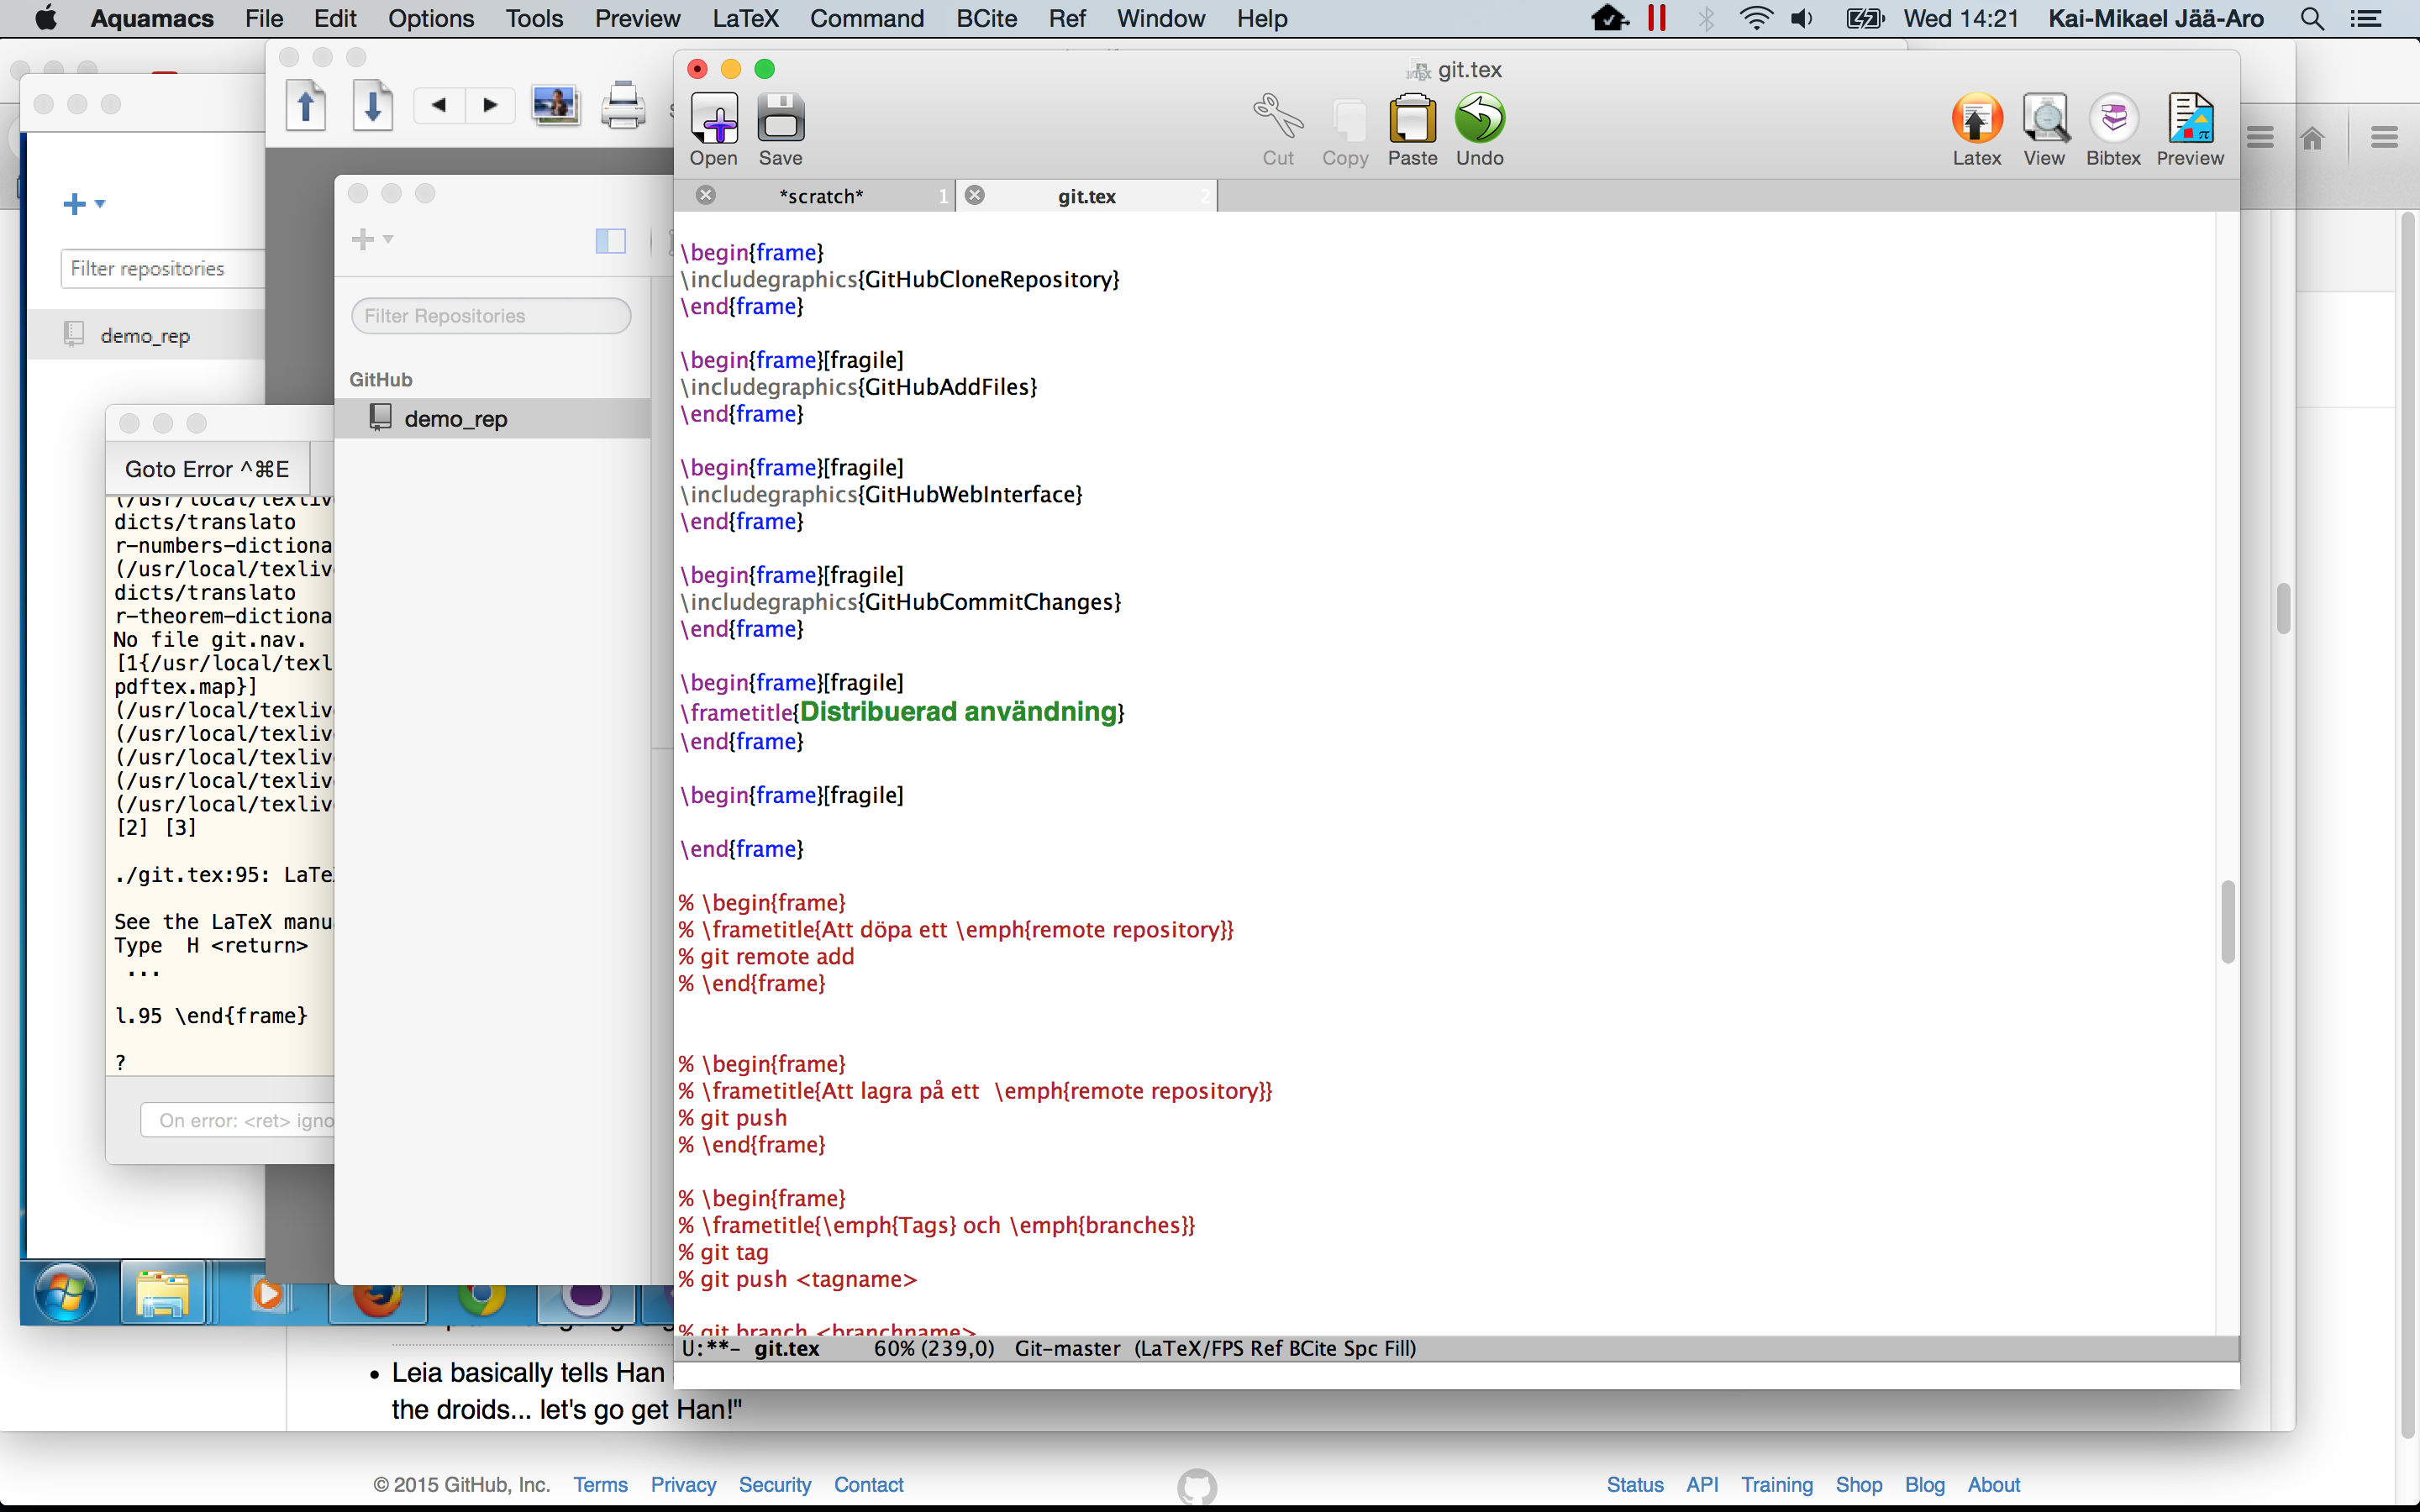
\includegraphics{EmacsConflictResolved}
\end{frame}

\begin{frame}[fragile]
\textbf{Obs!}
Git förstår bara filer som en sträng text.
Konflikter förstås som ändringar på samma position av flera utvecklare, men om någon skulle ändra
en funktion \lstinline+public void func1(int par1, int par2)+ till \lstinline+public void func1(int par1)+ invalideras alla anrop till \lstinline+func1+, men
git varnar inte för detta.

Därför bör alla incheckningar följas av ett \emph{bygge} för att
kontrollera att allt fortfarande fungerar.
\end{frame}

\begin{frame}
  \frametitle{Att ångra sig}
  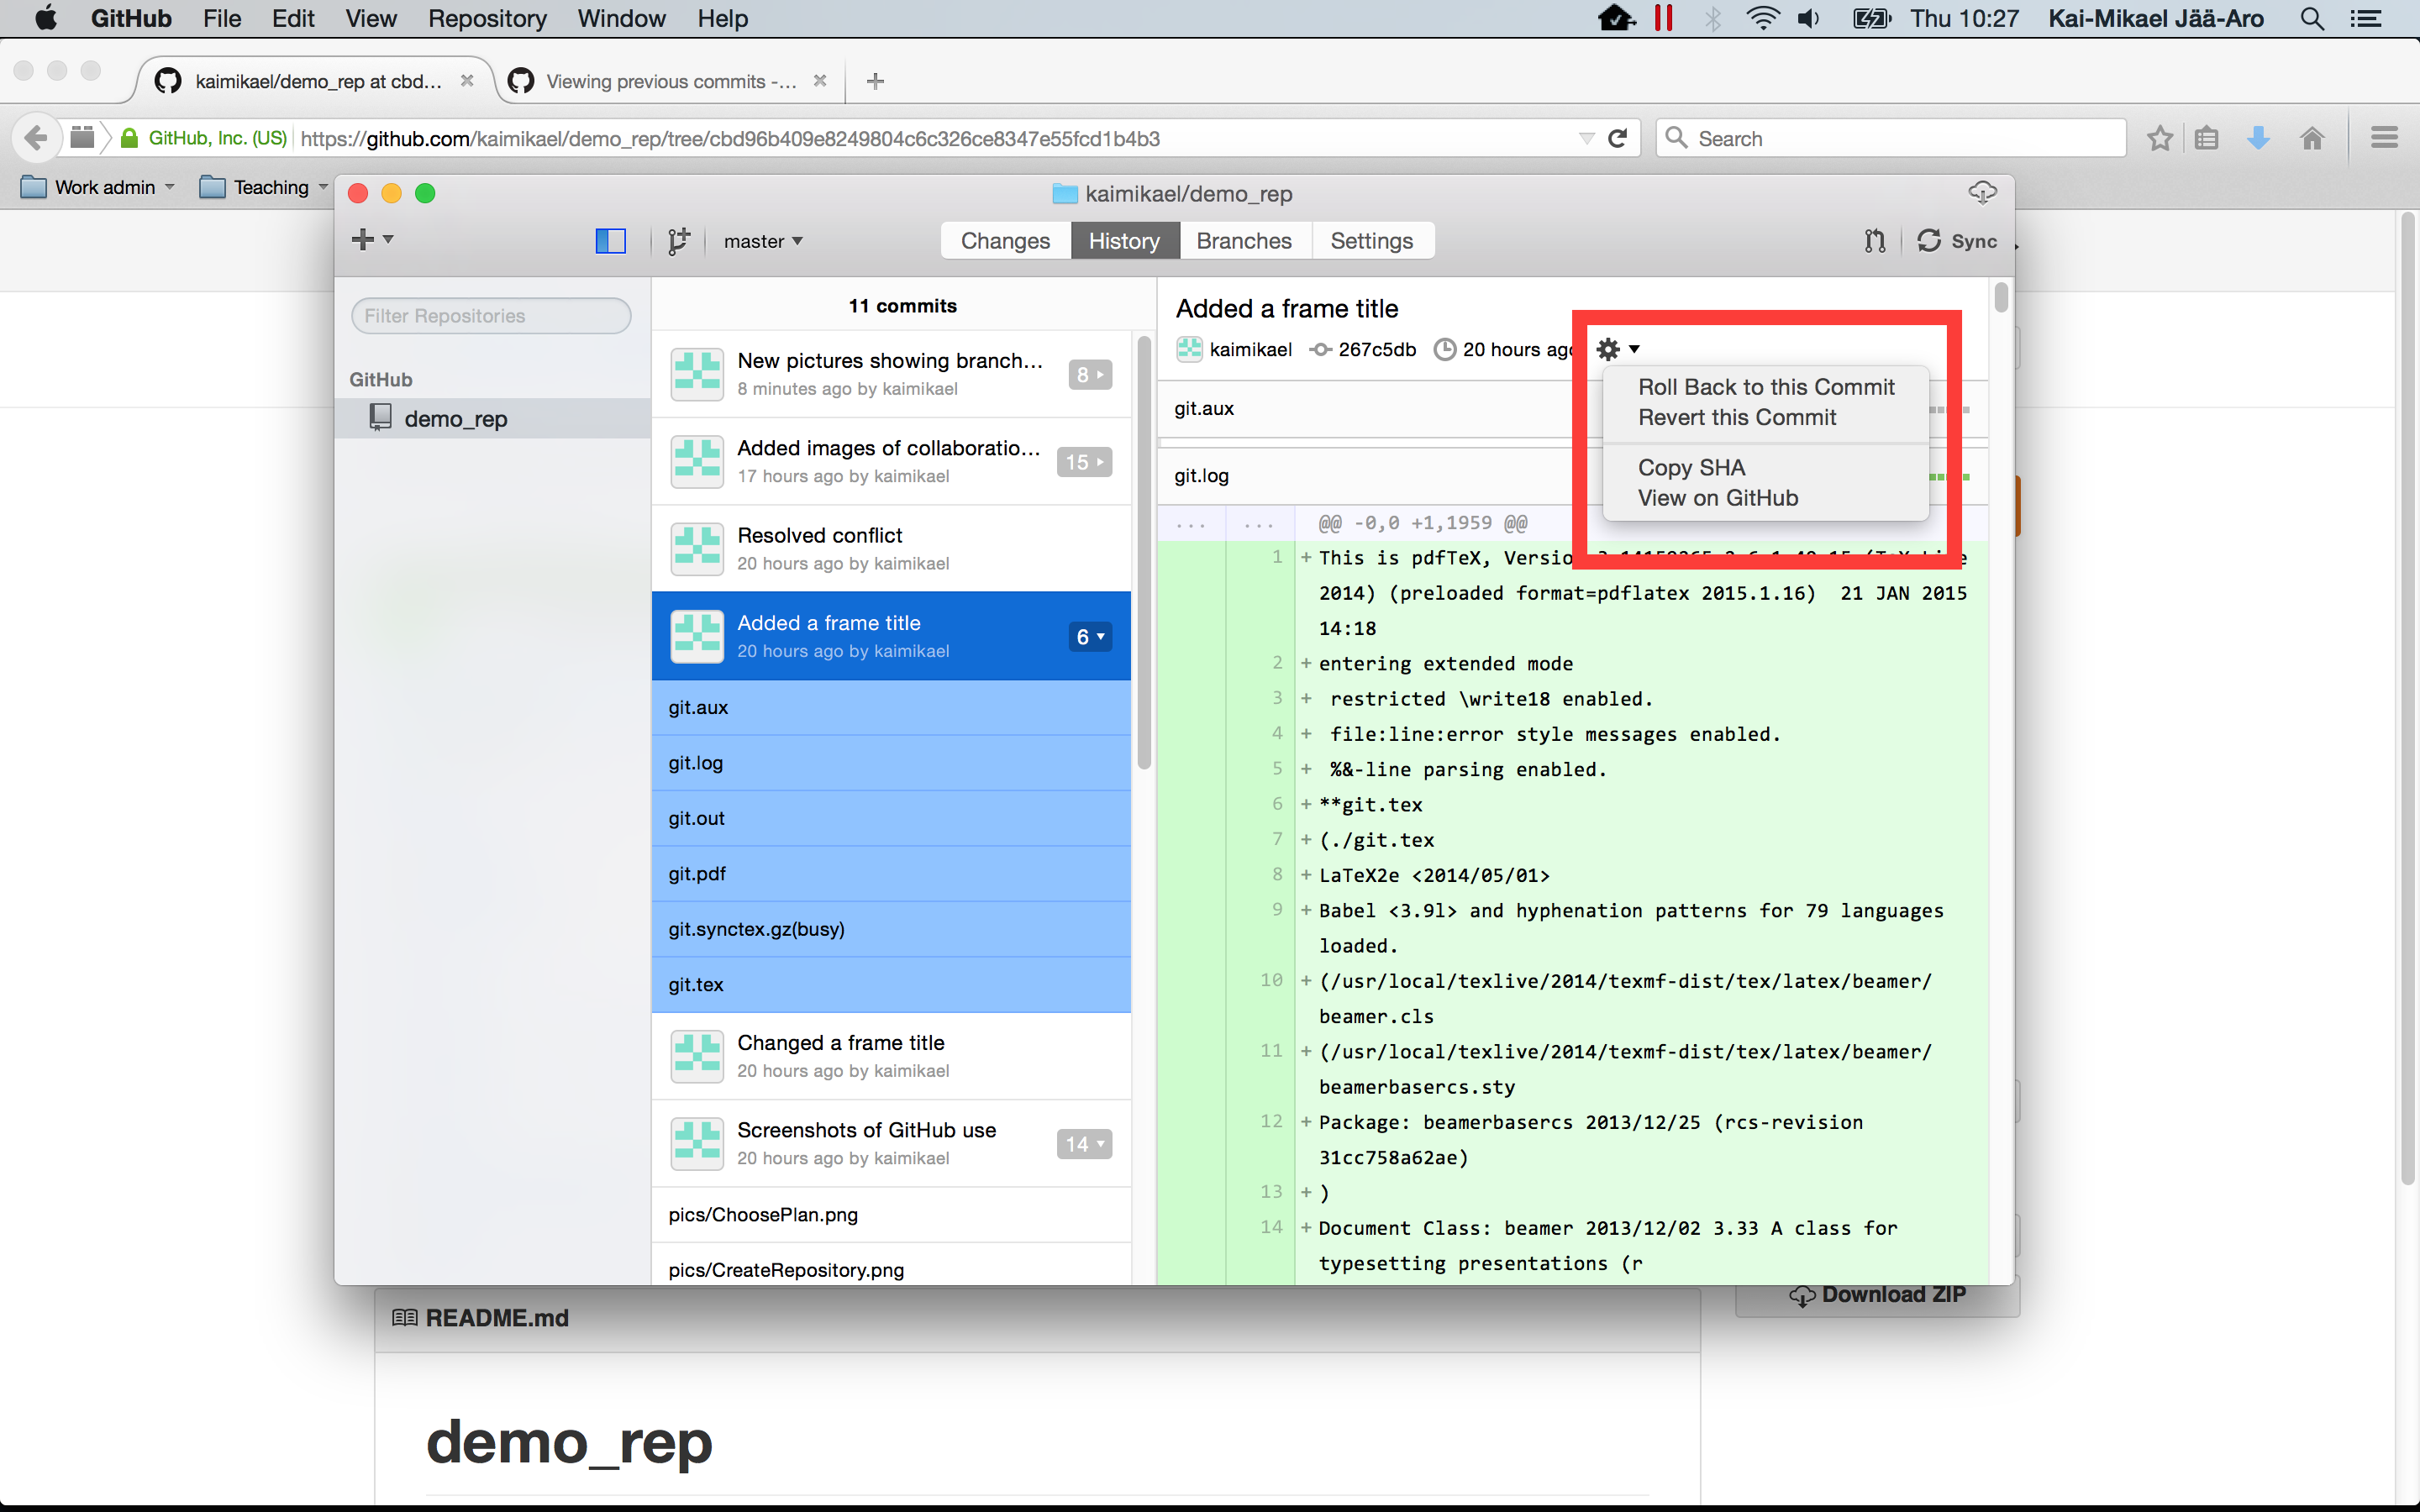
\includegraphics{GitHubRollback}
\end{frame}

\begin{frame}
\frametitle{Att ha en privat utvecklingsgren}
Ett vanligt arbetsflöde är att man har en \emph{master branch}, där koden är garanterad att vara stabil och körbar.  Olika utvecklare kan sedan lätt skapa en egen gren att koda och testa i.  Om något blir fel kan man alltid backa i denna gren och hålla mastern stabil.  Man kan självfallet göra ytterligare grenar för olika tester.

git-arkiven är uppbyggda så att de låter oss arbeta på vilken punkt i trädet vi vill.  Man kan se det som att man har en pekare in i trädet som pekar ut den aktuella uppsättningen filer som vi arbetar på.  Vid behov kan vi flytta pekaren nån annanstans och arbeta där istället.
\end{frame}

\begin{frame}
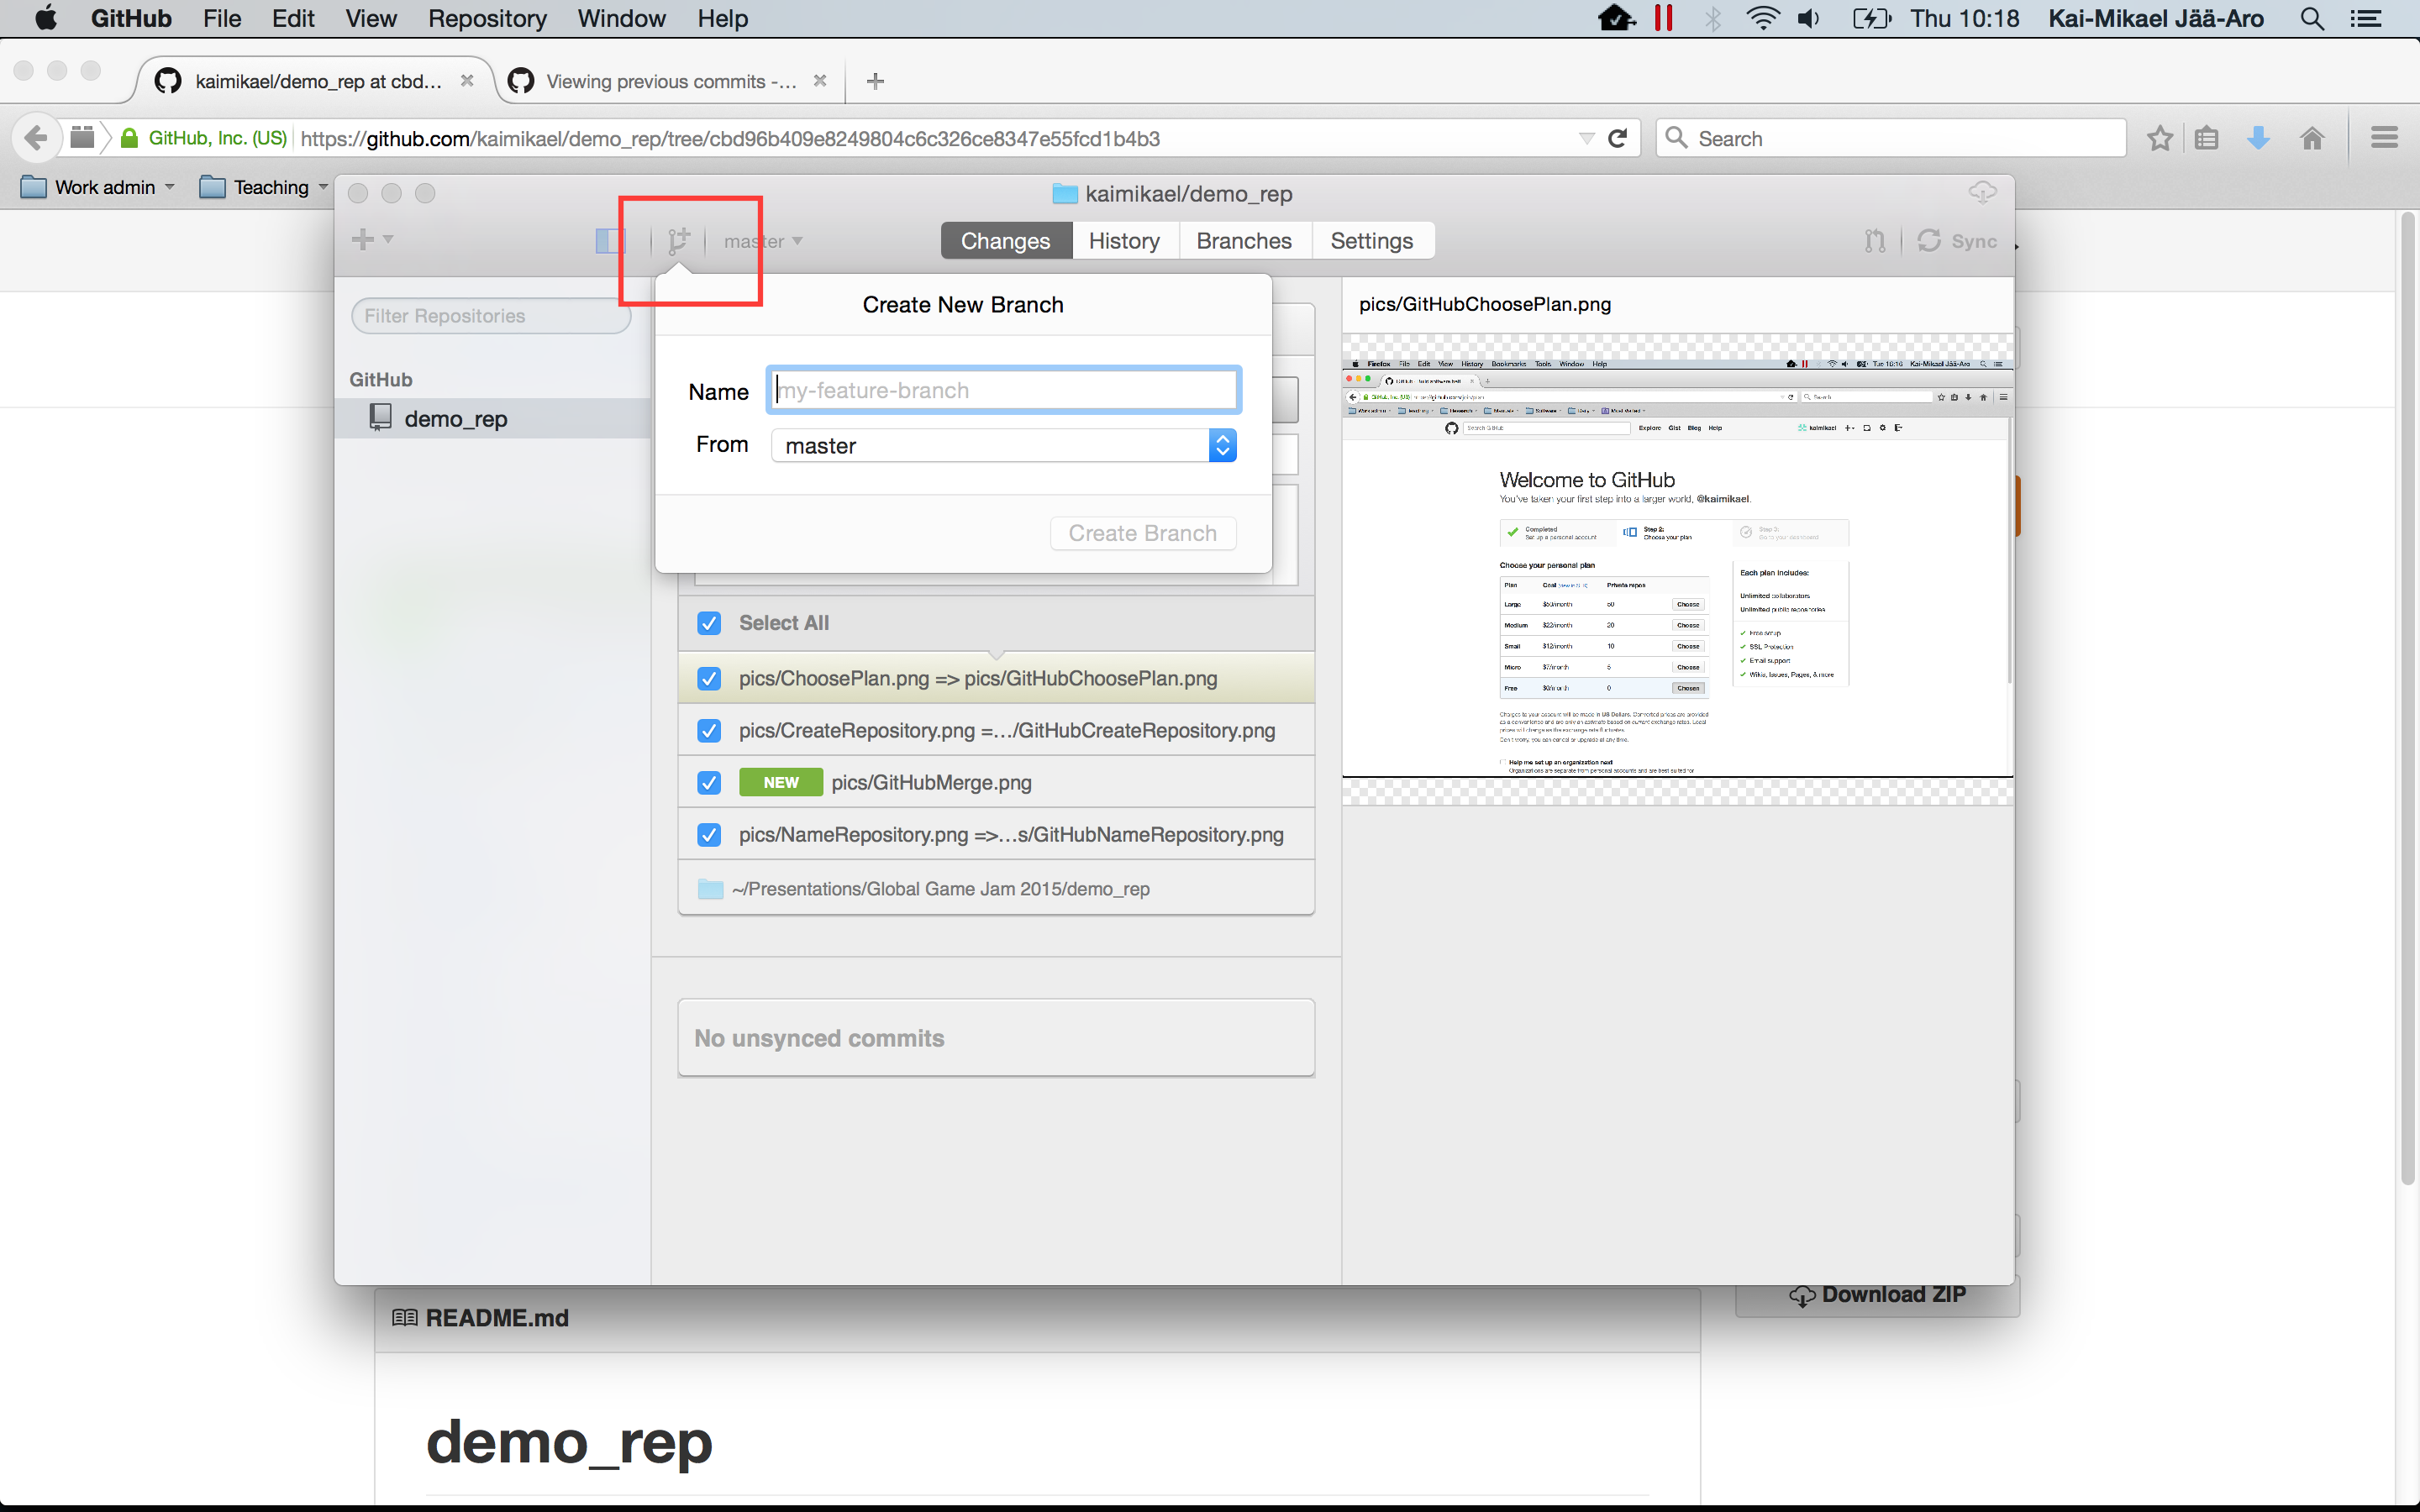
\includegraphics{GitHubCreateNewBranch}  
\end{frame}

\begin{frame}
\frametitle{\emph{Merge}}

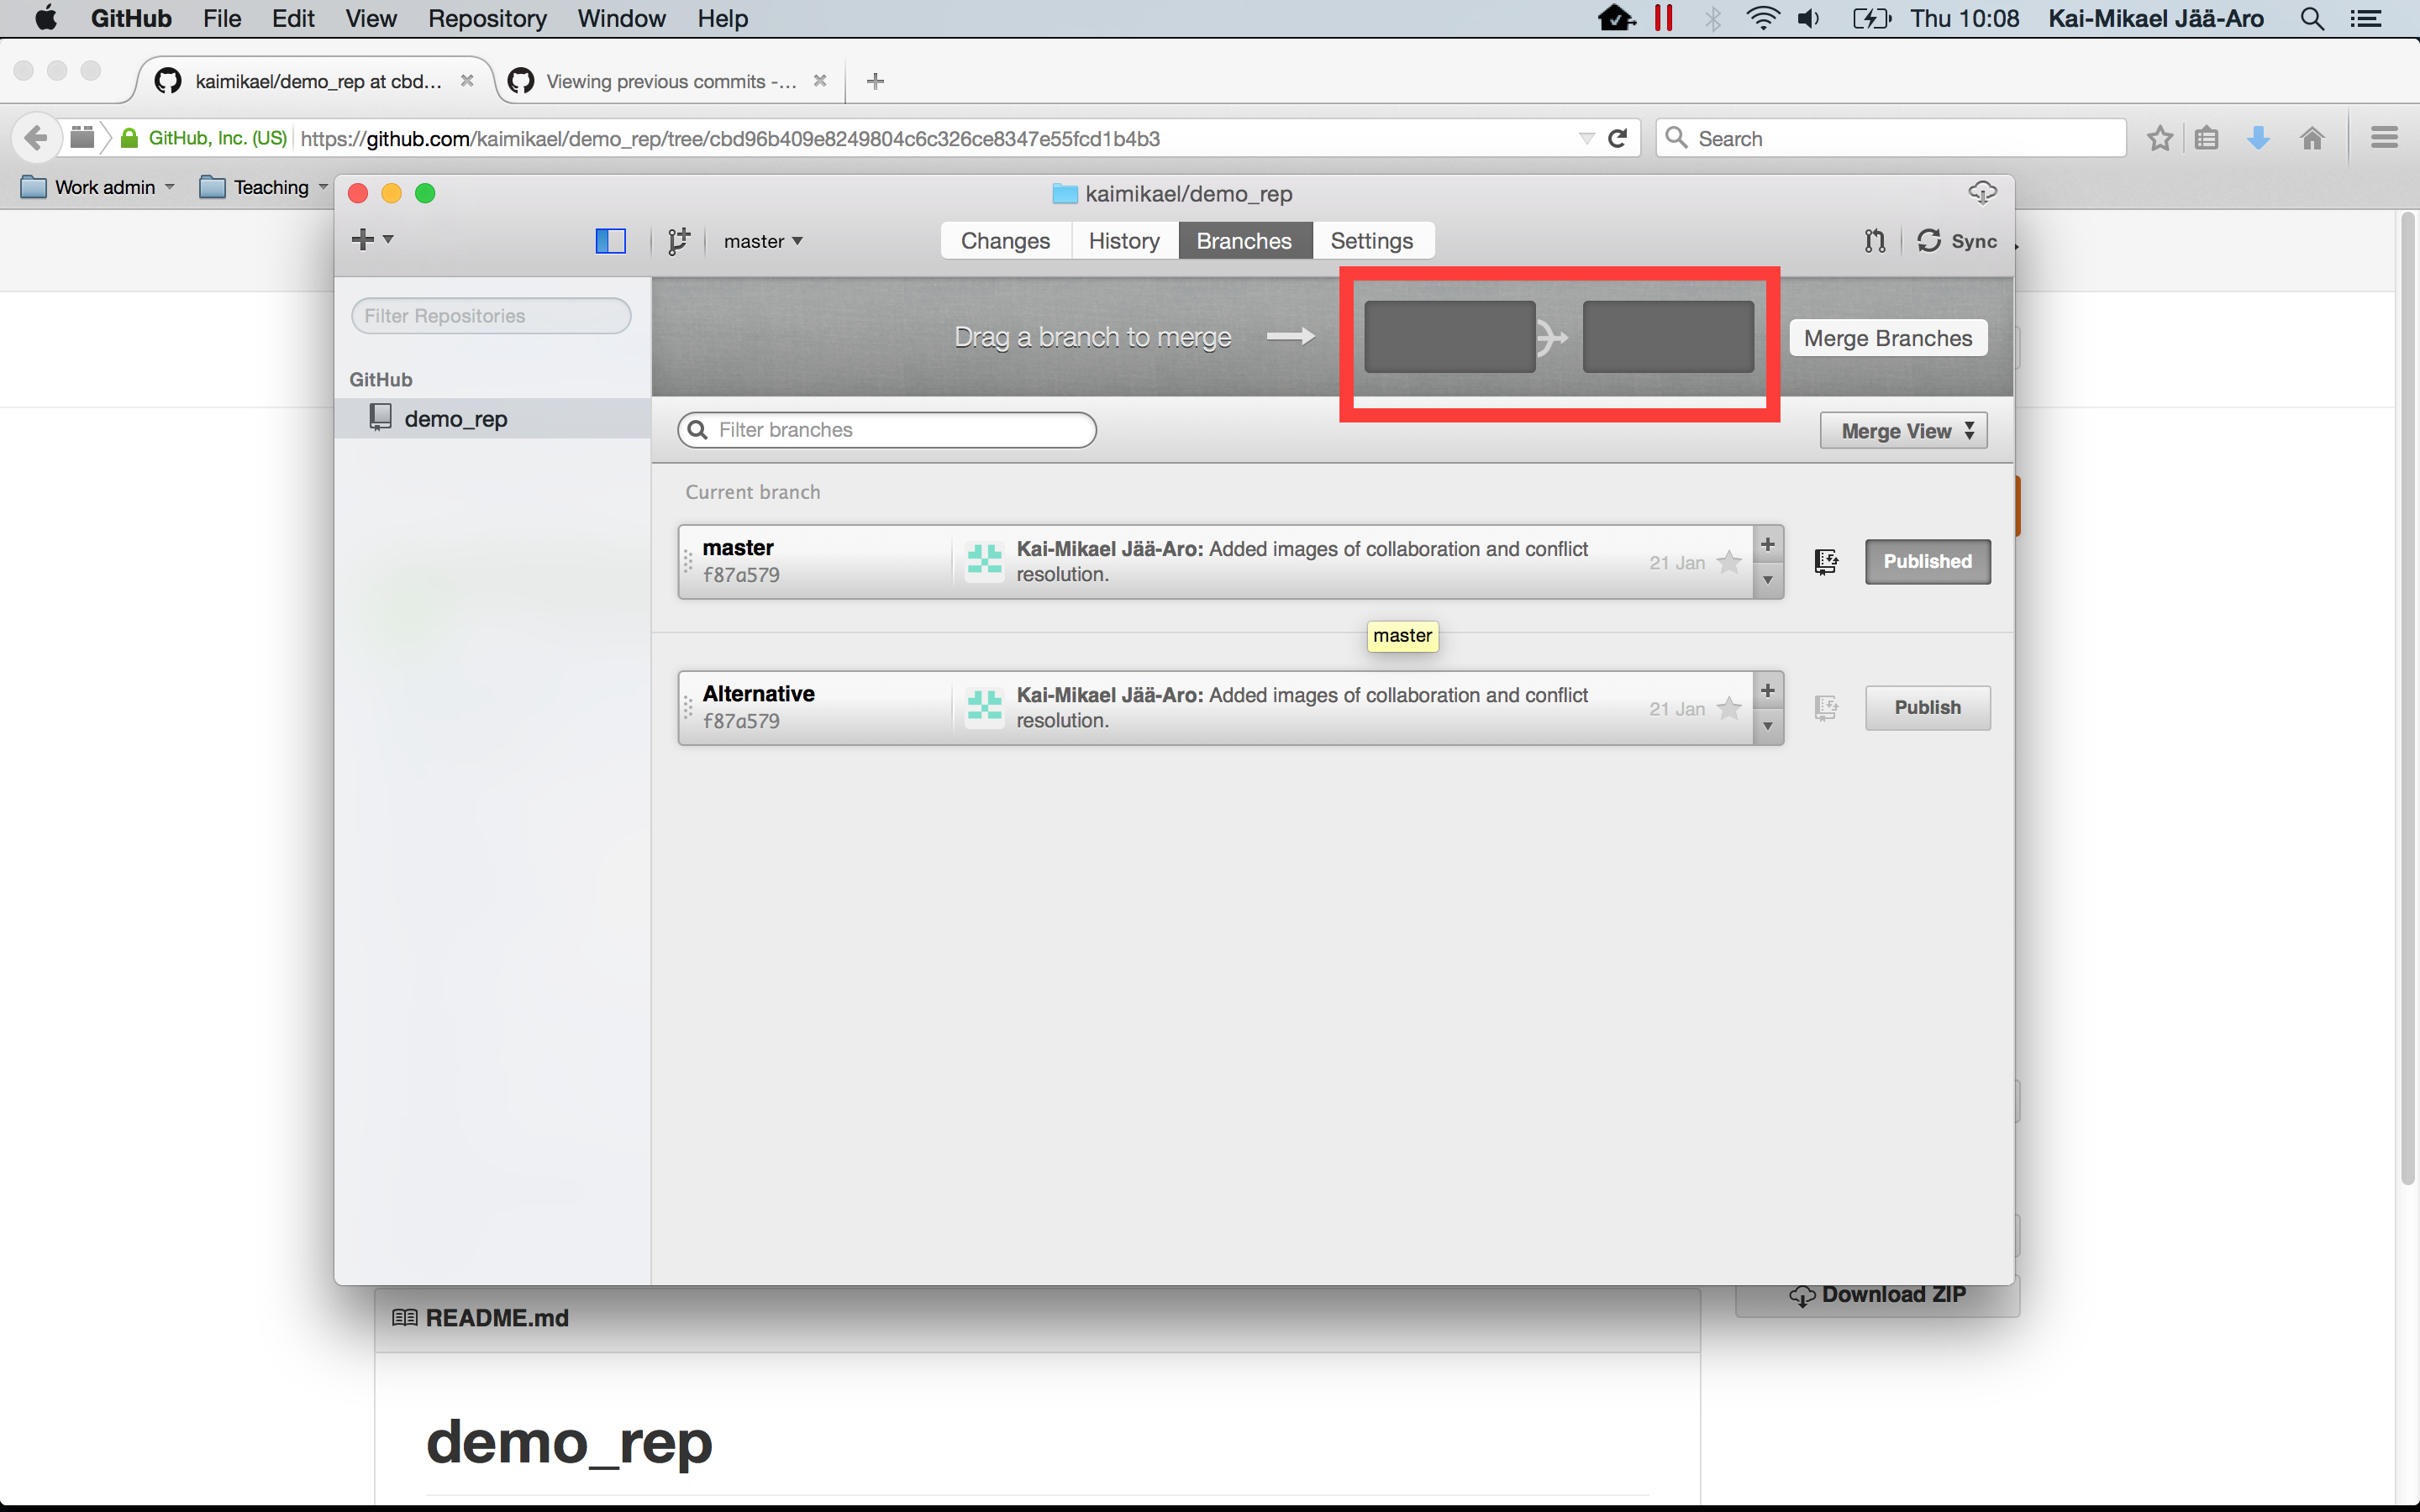
\includegraphics{GitHubMerge}

\end{frame}

\begin{frame}
\frametitle{\emph{merge} av binära filer}
git klarar inte av att göra merge på binära filer -- \mao texturer, animationer, \odyl.  Somliga installationer kan ha en mergetool som kan hjälpa till, men i allmänhet måste man manuellt hämta de binära filer man vill ha.
  
\end{frame}


\begin{frame}
\frametitle{Mer läsning}  
\href{http://git-scm.com/book/en/v2/}{\textsl{Pro Git, 2nd Edition}, Scott Chacon \& Ben Straub.}
\end{frame}
\end{document}
